\documentclass{article}
\usepackage[utf8]{inputenc}
\usepackage[margin =30 mm ]{ geometry }
\usepackage{graphicx}
\usepackage{amsmath}
\usepackage{hyperref}
\usepackage{float}
\usepackage{wrapfig}
\usepackage{subcaption}
\usepackage{listings}
\usepackage{multirow}
\setlength{\parindent}{1cm}
% chktex-file 36
% chktex-file 12
% chktex-file 24
% chktex-file 44
% chktex-file 18
% chktex-file 8
% chktex-file 13
\title{Position sensitive scintillator detectors for gamma ray imaging}
\author{Tasks and results}
\date{November 2023}

\begin{document}

\maketitle

\section{Tasks:}

\begin{enumerate}
    \item Introducere
        \begin{itemize}
            \item Build and run example TestEM4 in batch mode also in visualization mode. Save and plot results
            \item Define new materials: CsI (Tl), BGO, LYSO
            \item Define a panel scintillator of 4 cm 4 cm x 2 mm
            \item Simulate the deposited energy in each type of scintillator for photon energies: 0.1 MeV, 0.5 MeV, 1 MeV, 3 MeV, 5 MeV, 10 MeV
            \item Plot all results
        \end{itemize}
    \item Calcularea energiei depuse
        \begin{itemize}
            \item Sursa --- fascicul dicrectionat pe axa z, fara deschidere unghiulara
            \item Pentru mai multe grosimi ale scintilatorului, calculeaza energia depusa
            \item Scrie un cod in Python care sa calculeze Edep
            \item $E_{dep} = \sum_{i} entries_i \cdot E_i$
            \item Plot all results
        \end{itemize}
    \item Optical yield
        \begin{itemize}
            \item Materiale: [BGO, CsI (Tl), BGO]; grosimi: [0.5, 1, 2] mm; energii: [0.1, 0.5, 1, 3, 5, 10] MeV
            \item Calculand probabilitatea de interactie, afla numarul de fotoni care interactioneaza si compara cu numarul de entries dat de G4
            \item $\text{Interactii} = N_0(1-e^{-\mu x})$
            \item Coeficientii de atenuare liniara --- din baza de date nist xcom
            \item Pentru fiecare energie depusa calculata, sa se calculeze si numarul de scintilatii (numarul de fotoni optici creati) cunoscand light yield-ul fiecarui material
            \item Scrie un cod care sa parcurga toate fisierele, care sunt denumite in forma:
            
            \verb|MATERIAL_ENERGY_WIDTH.root|
            
            \item Plot all results
        \end{itemize}
    \item Suprafata in care s-a depus energia
        \begin{itemize}
            \item Studiaza depunerea de energie salvand datele intr-o histograma 2D: poxitia (x,y) + Edep
            \item Facand proiectia pe axele x si y, calculeaza FWHM din profilul 1D
            \item Realizeaza graficul FWHM in functie de energie si grosime/scintilator
            \item[*] Realizeaza un fit in python cu o functie Lorentziana/Super Gaussiana
            \item[*] Pentru funcția Lorentziana, FWHM = $2 \cdot \gamma$. 
            \item[*] Realizeaza simulari pentru diferite energii, grosimi si scintilatori
            \item[*] Mareste numarul de bini din histograma (redu dimensiunile scintilatorului) 
            \item[*] Analitic, afla FWHM si FWTM.
        \end{itemize}
\end{enumerate}

\newpage

\section{Results}

\subsection{Task 1. Photon energy deposition in a scintillator panel made of CsI (Tl), BGO or LYSO}

\begin{figure}[H]
    \centering
    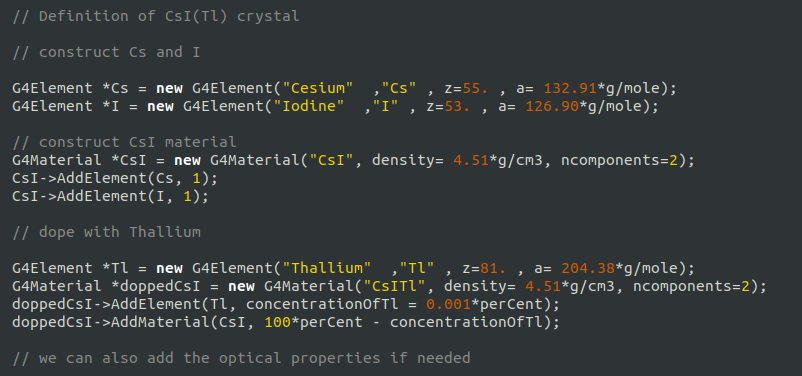
\includegraphics[width=\linewidth]{images//task1/material_CSI.png}
    \caption{Define material --- CsI (Tl)}
    \label{fig:matCSI}
\end{figure}
\begin{figure}[H]
        \centering
        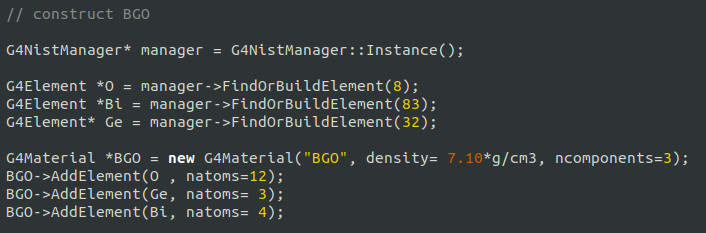
\includegraphics[width=\linewidth]{images//task1/material_BGO.png}
        \caption{Define material - BGO}
        \label{fig:matBGO}
\end{figure}
\begin{figure}[H]
    \centering
    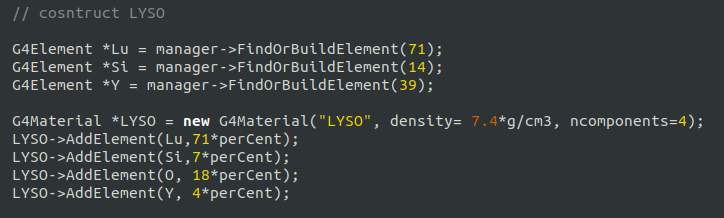
\includegraphics[width=\linewidth]{images//task1/material_LYSO.png}
    \caption{Define material - LYSO}
    \label{fig:matLYSO}
\end{figure}
\begin{figure}[H]
    \centering
    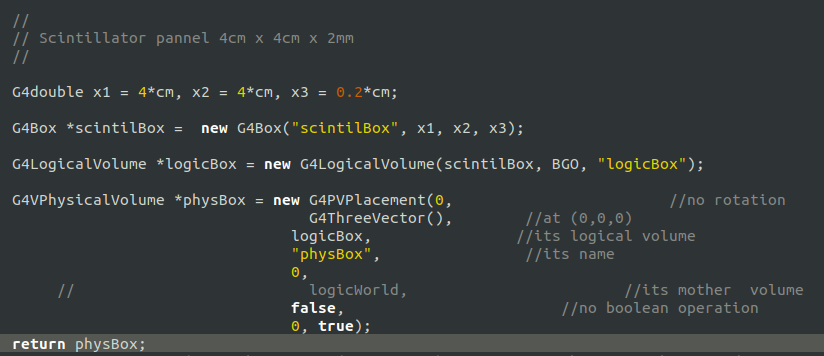
\includegraphics[width=1\linewidth]{images//task1/pannel_dimensions.png}
    \caption{Panel dimensions}
    \label{fig:dimensions}
\end{figure}

\subsubsection{CsI(Tl)}
\begin{figure}[H]
\centering
\begin{subfigure}{.5\textwidth}
  \centering
  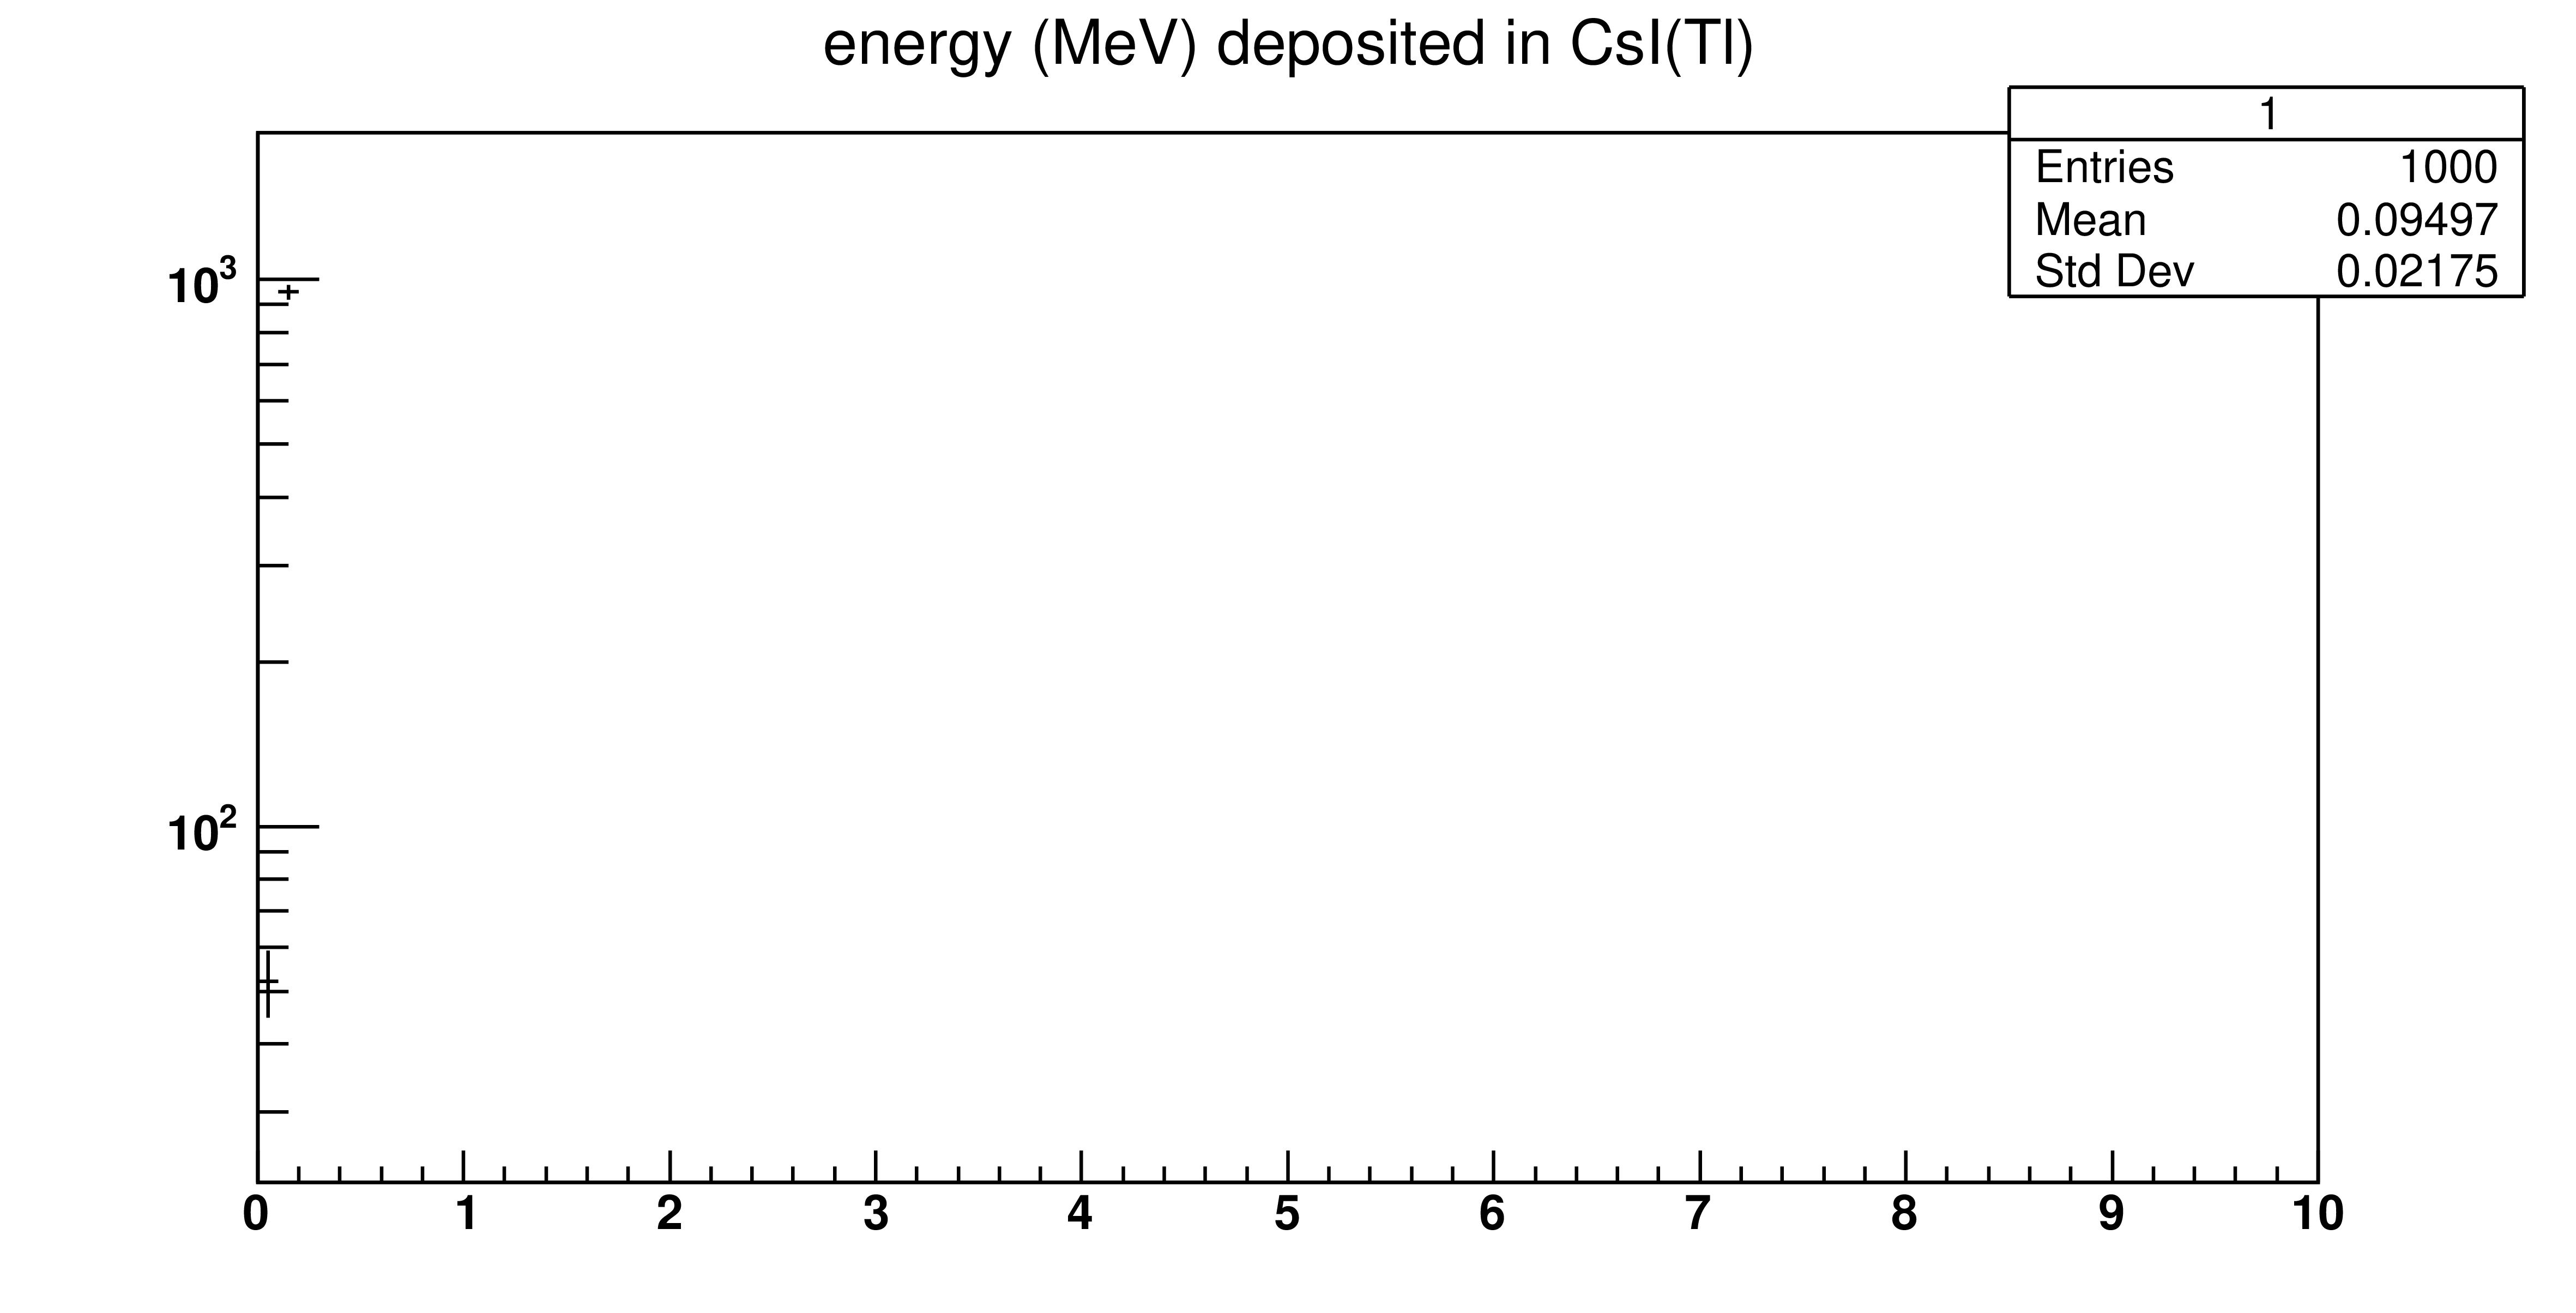
\includegraphics[width=\linewidth]{images/task1/CsI_01MeV.png}
  \caption{Deposited energy in CsI(Tl) at 0.1 MeV incident energy}
\end{subfigure}%
\begin{subfigure}{.5\textwidth}
  \centering
  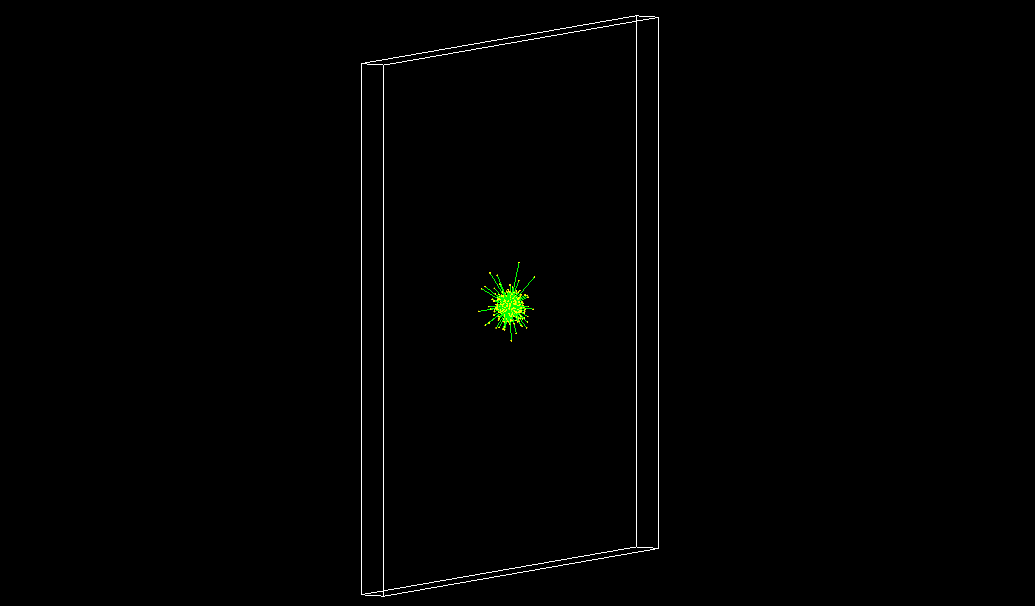
\includegraphics[width=\linewidth]{images/task1/CsI_01MeV_1000.png}
  \caption{Visualisation of the particle tracks}
\end{subfigure}
\caption{Results – CsI(Tl) – 0.1 MeV}
\end{figure}

\begin{figure}[H]
\centering
\begin{subfigure}{.5\textwidth}
  \centering
  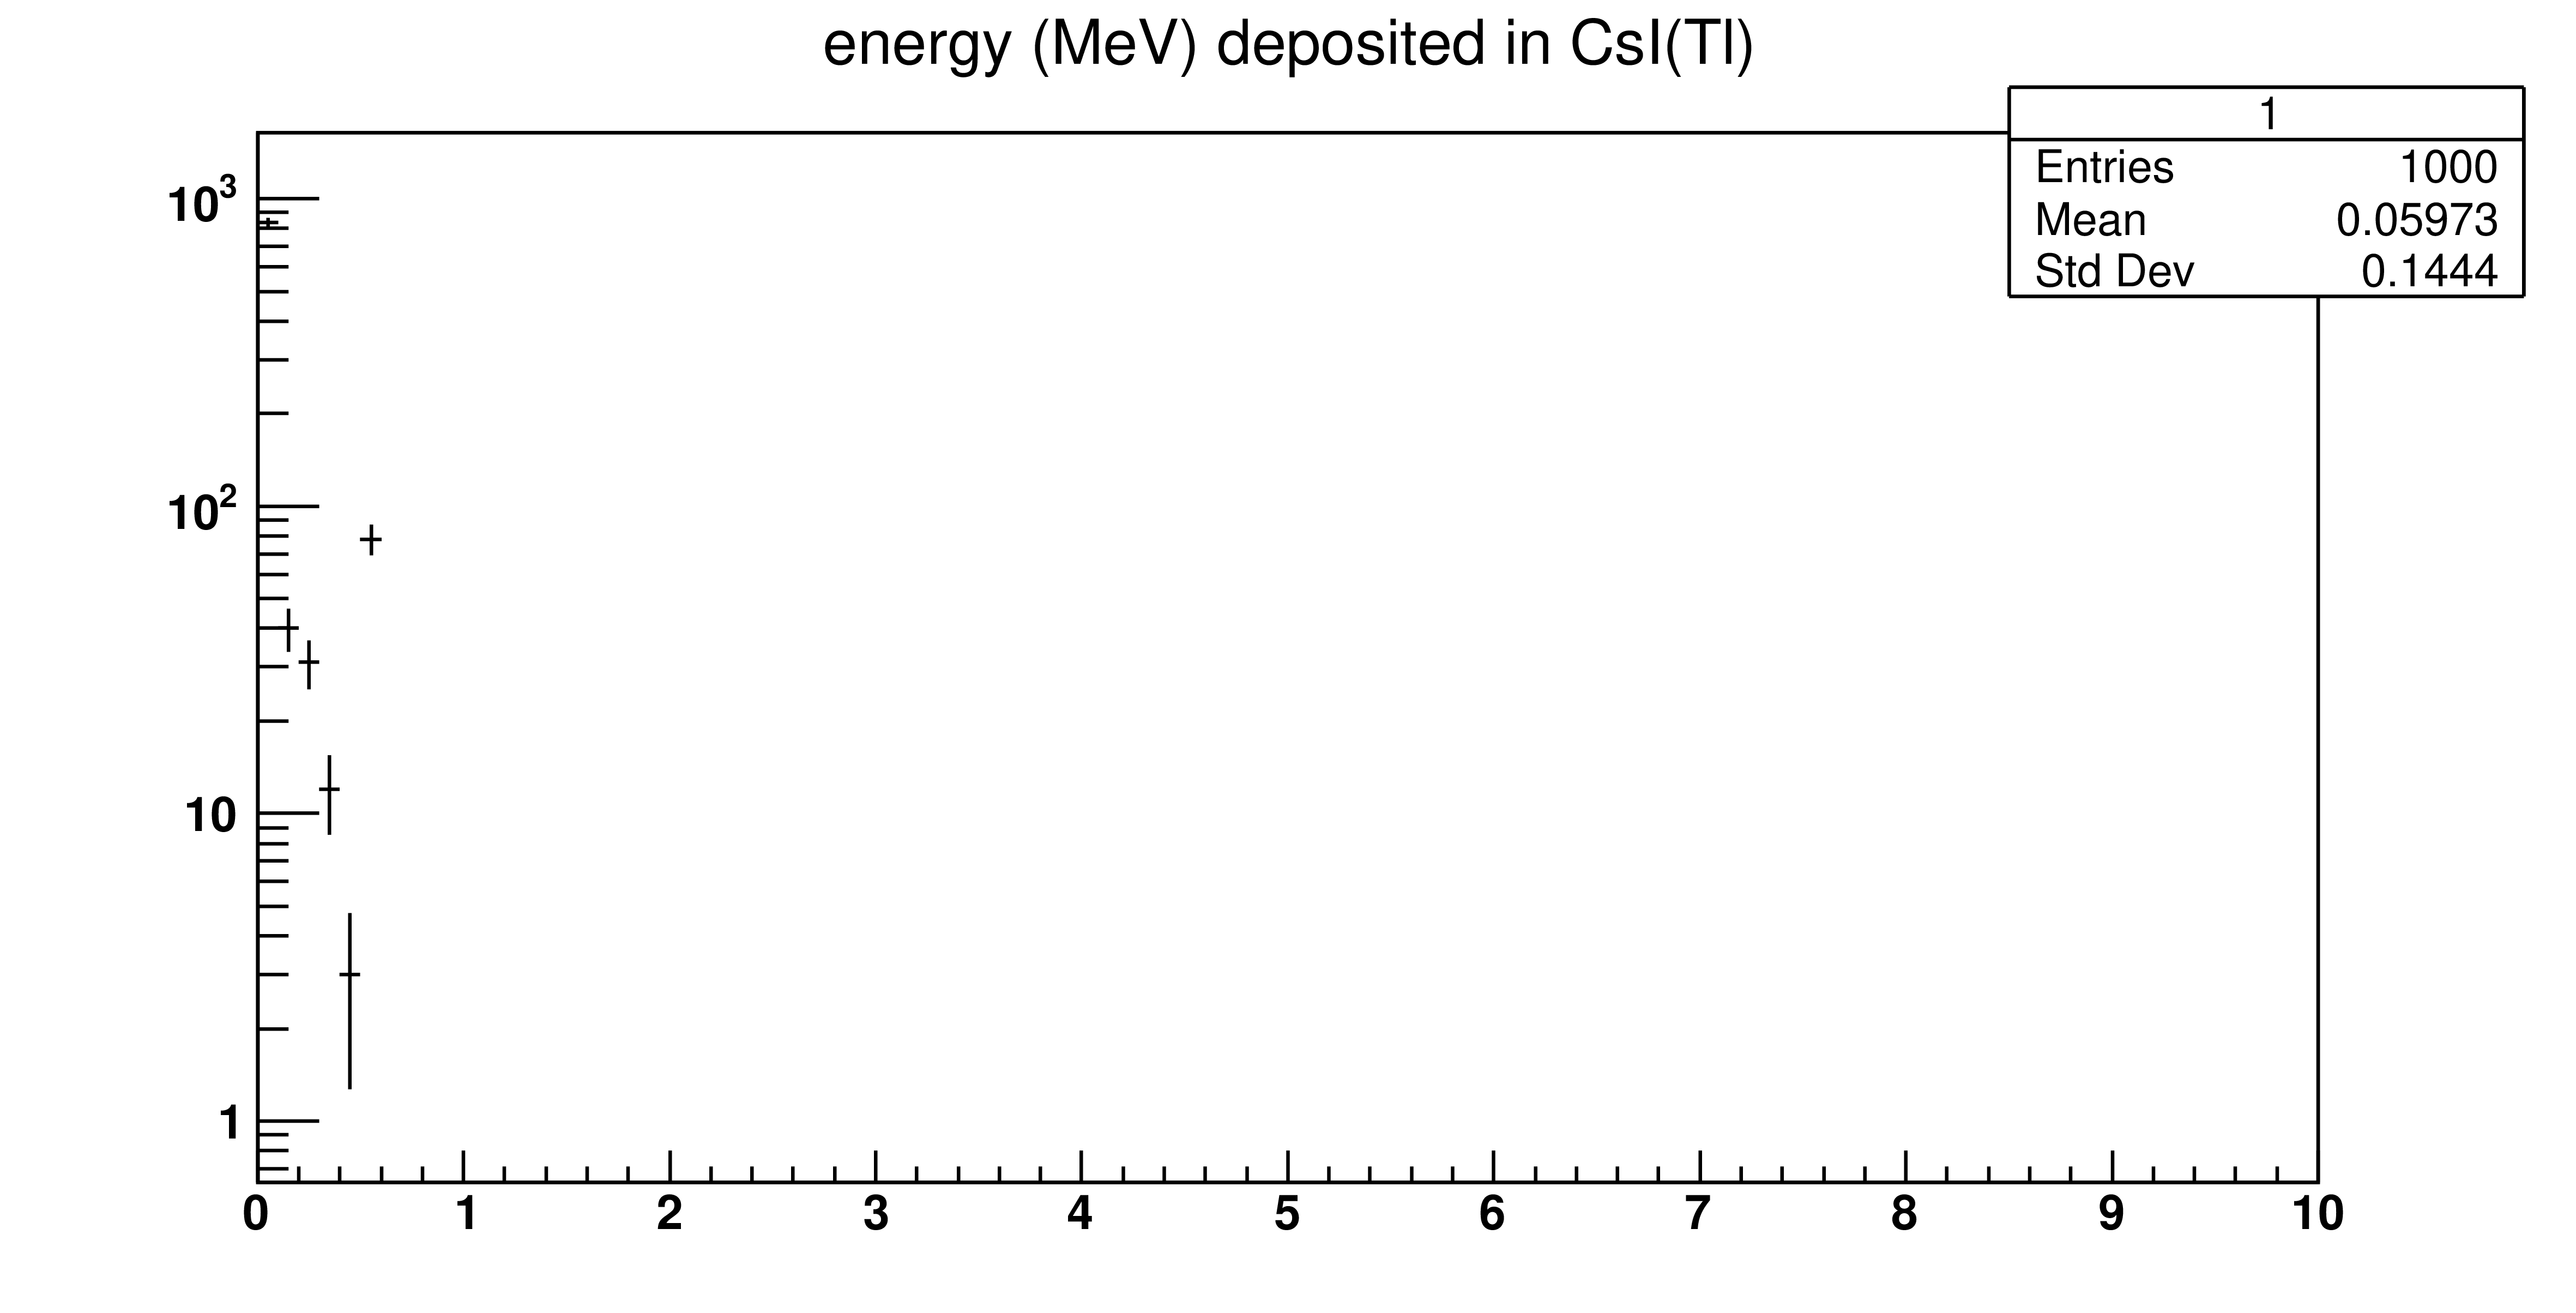
\includegraphics[width=\linewidth]{images/task1/CsI_05MeV.png}
  \caption{Deposited energy in CsI(Tl) at 0.5 MeV incident energy}
\end{subfigure}%
\begin{subfigure}{.5\textwidth}
  \centering
  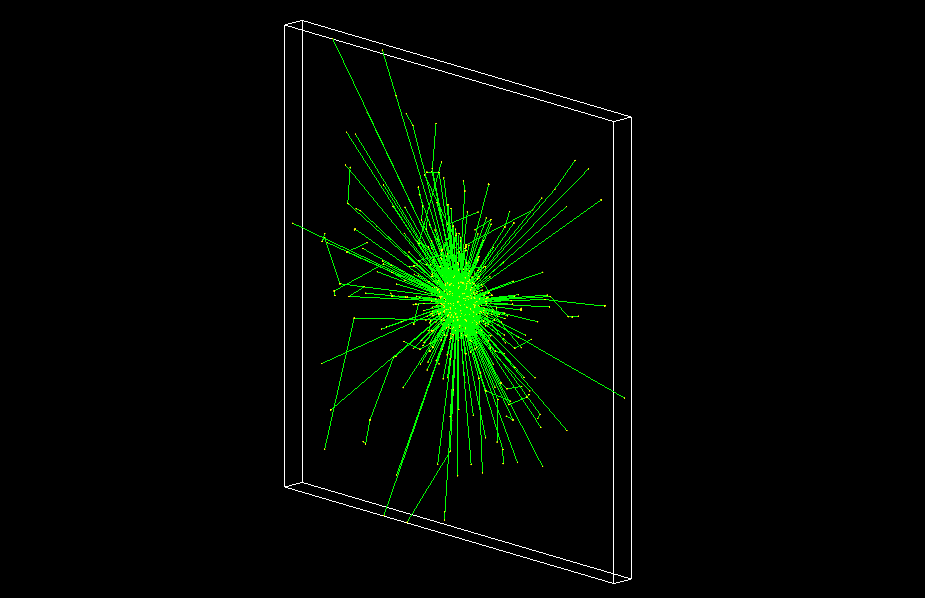
\includegraphics[width=\linewidth]{images/task1/CsI_05MeV_1000.png}
  \caption{Visualisation of the particle tracks}
\end{subfigure}
\caption{Results – CsI(Tl) – 0.5 MeV}
\end{figure}

\begin{figure}[H]
\centering
\begin{subfigure}{.5\textwidth}
  \centering
  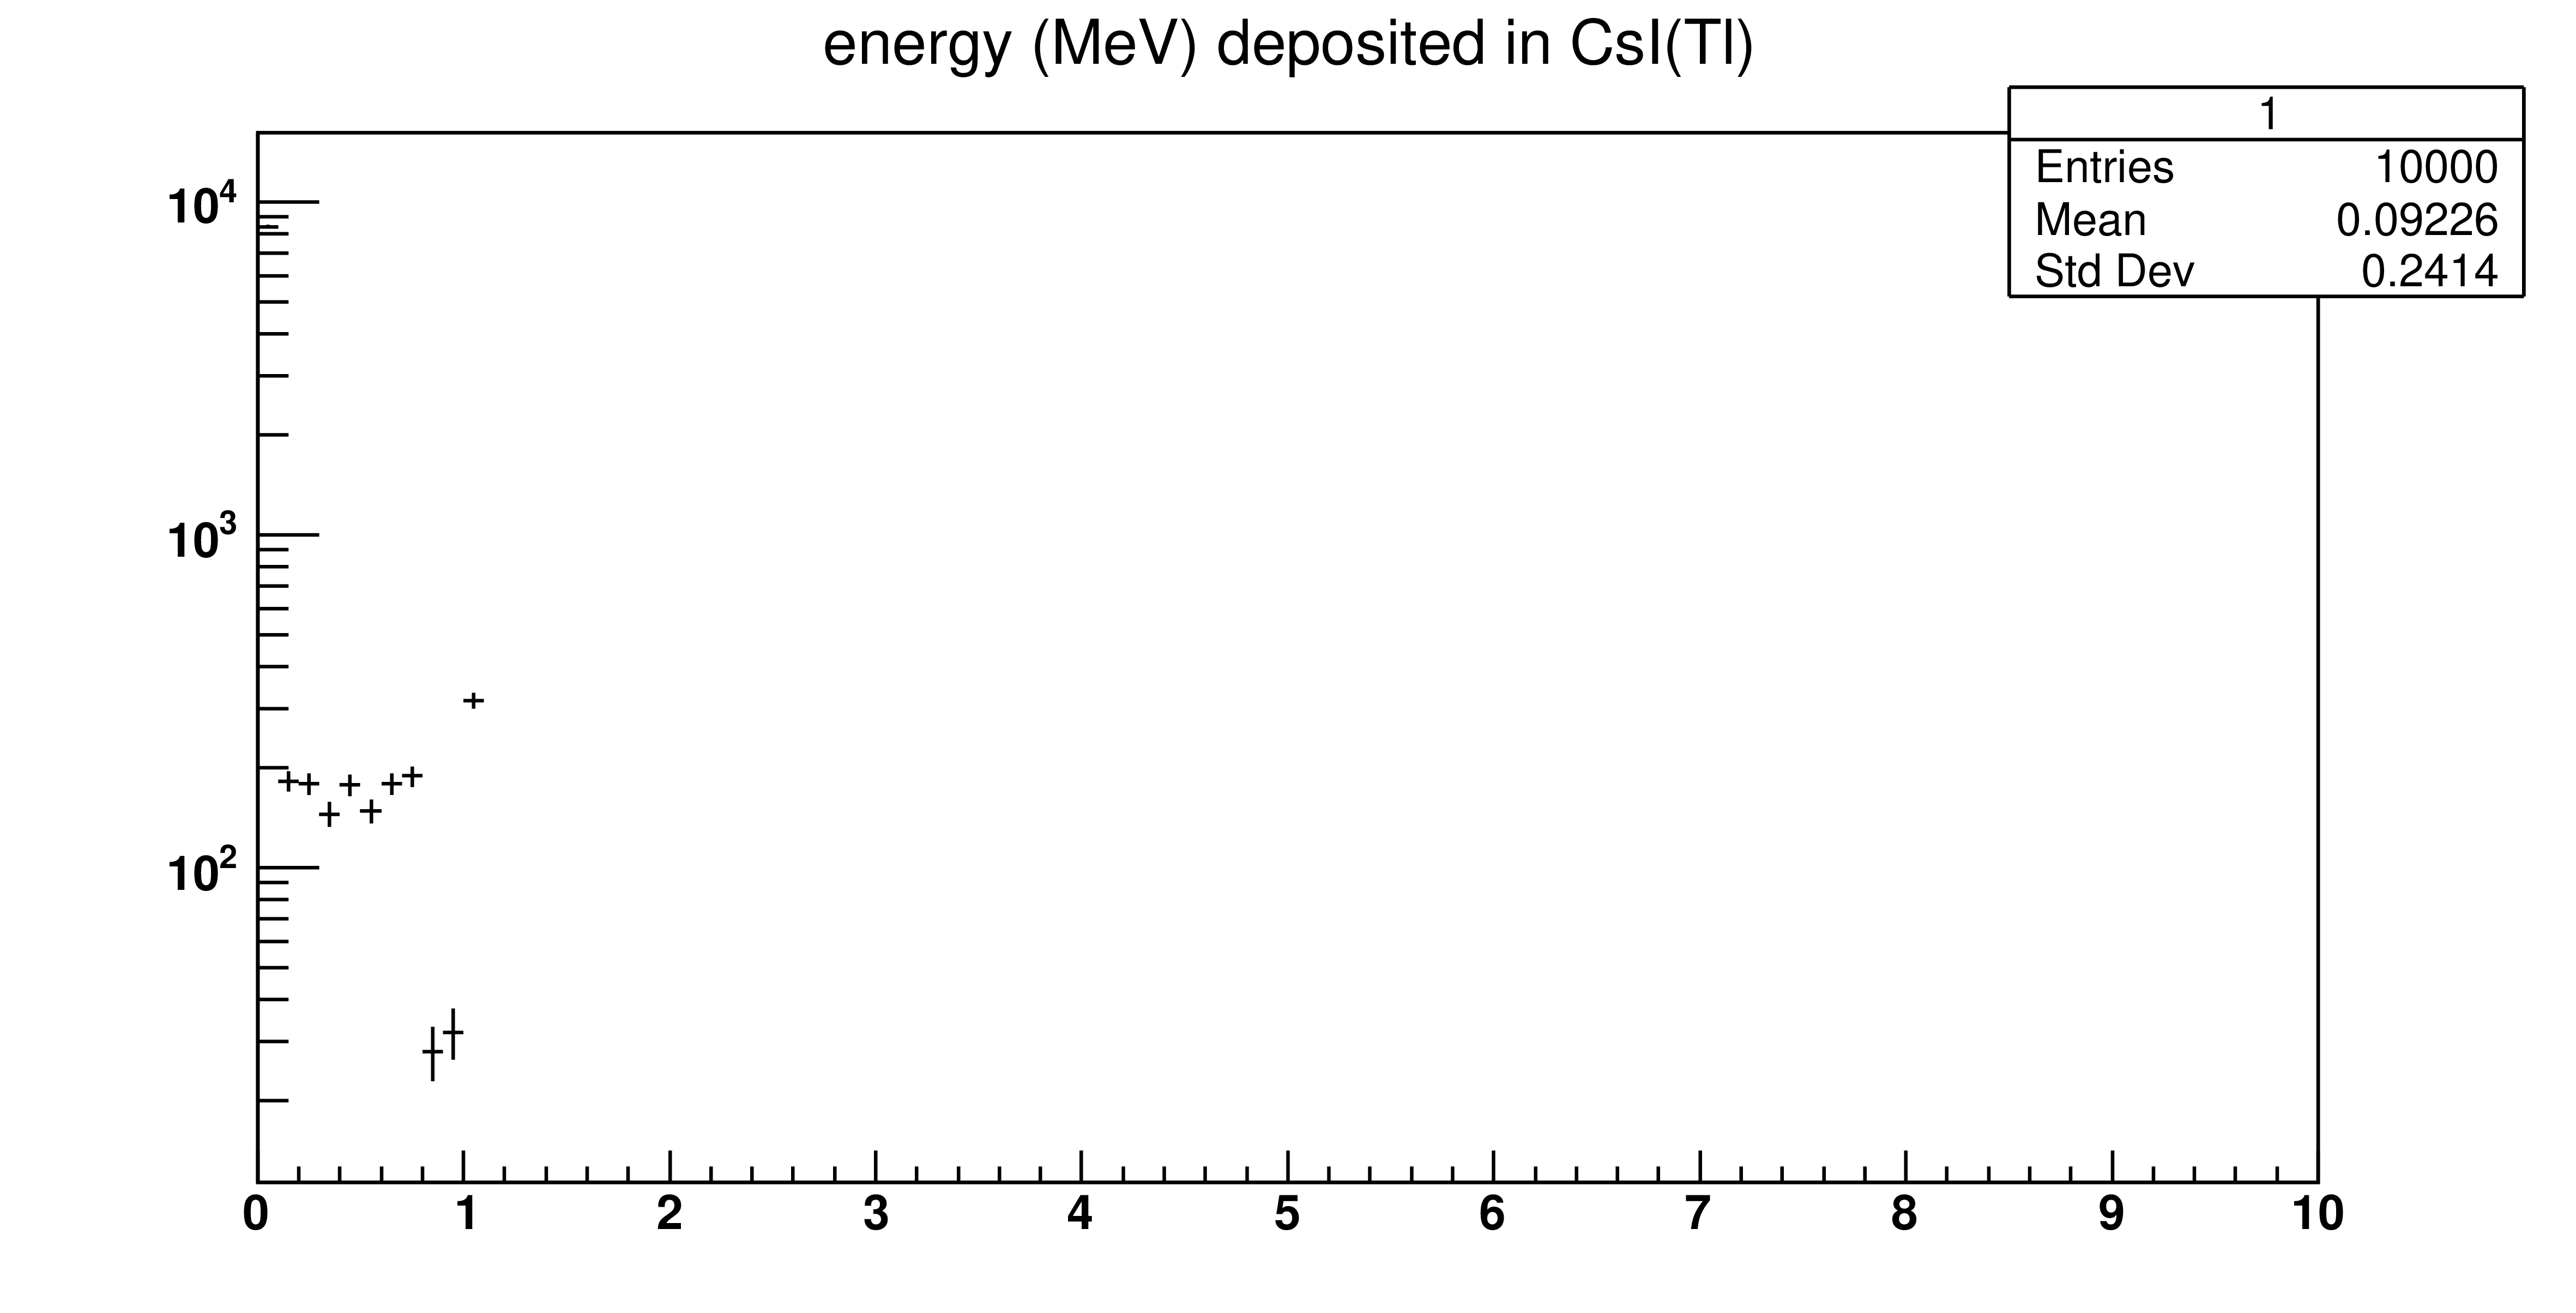
\includegraphics[width=\linewidth]{images/task1/CsI_1MeV.png}
  \caption{Deposited energy in CsI(Tl) at 1 MeV incident energy}
\end{subfigure}%
\begin{subfigure}{.5\textwidth}
  \centering
  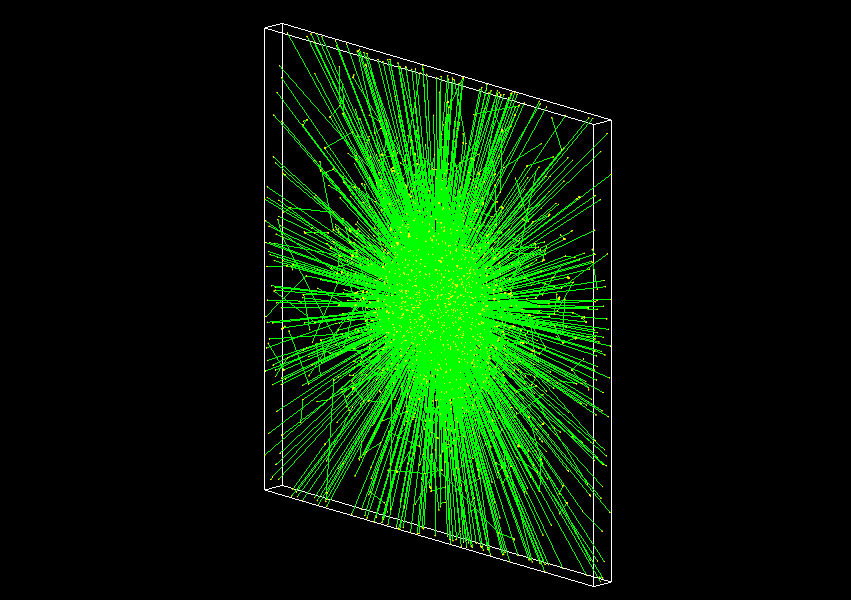
\includegraphics[width=\linewidth]{images/task1/CsI_1MeV_10000.png}
  \caption{Visualisation of the particle tracks}
\end{subfigure}
\caption{Results – CsI(Tl) – 1 MeV}
\end{figure}

\begin{figure}[H]
\centering
\begin{subfigure}{.5\textwidth}
  \centering
  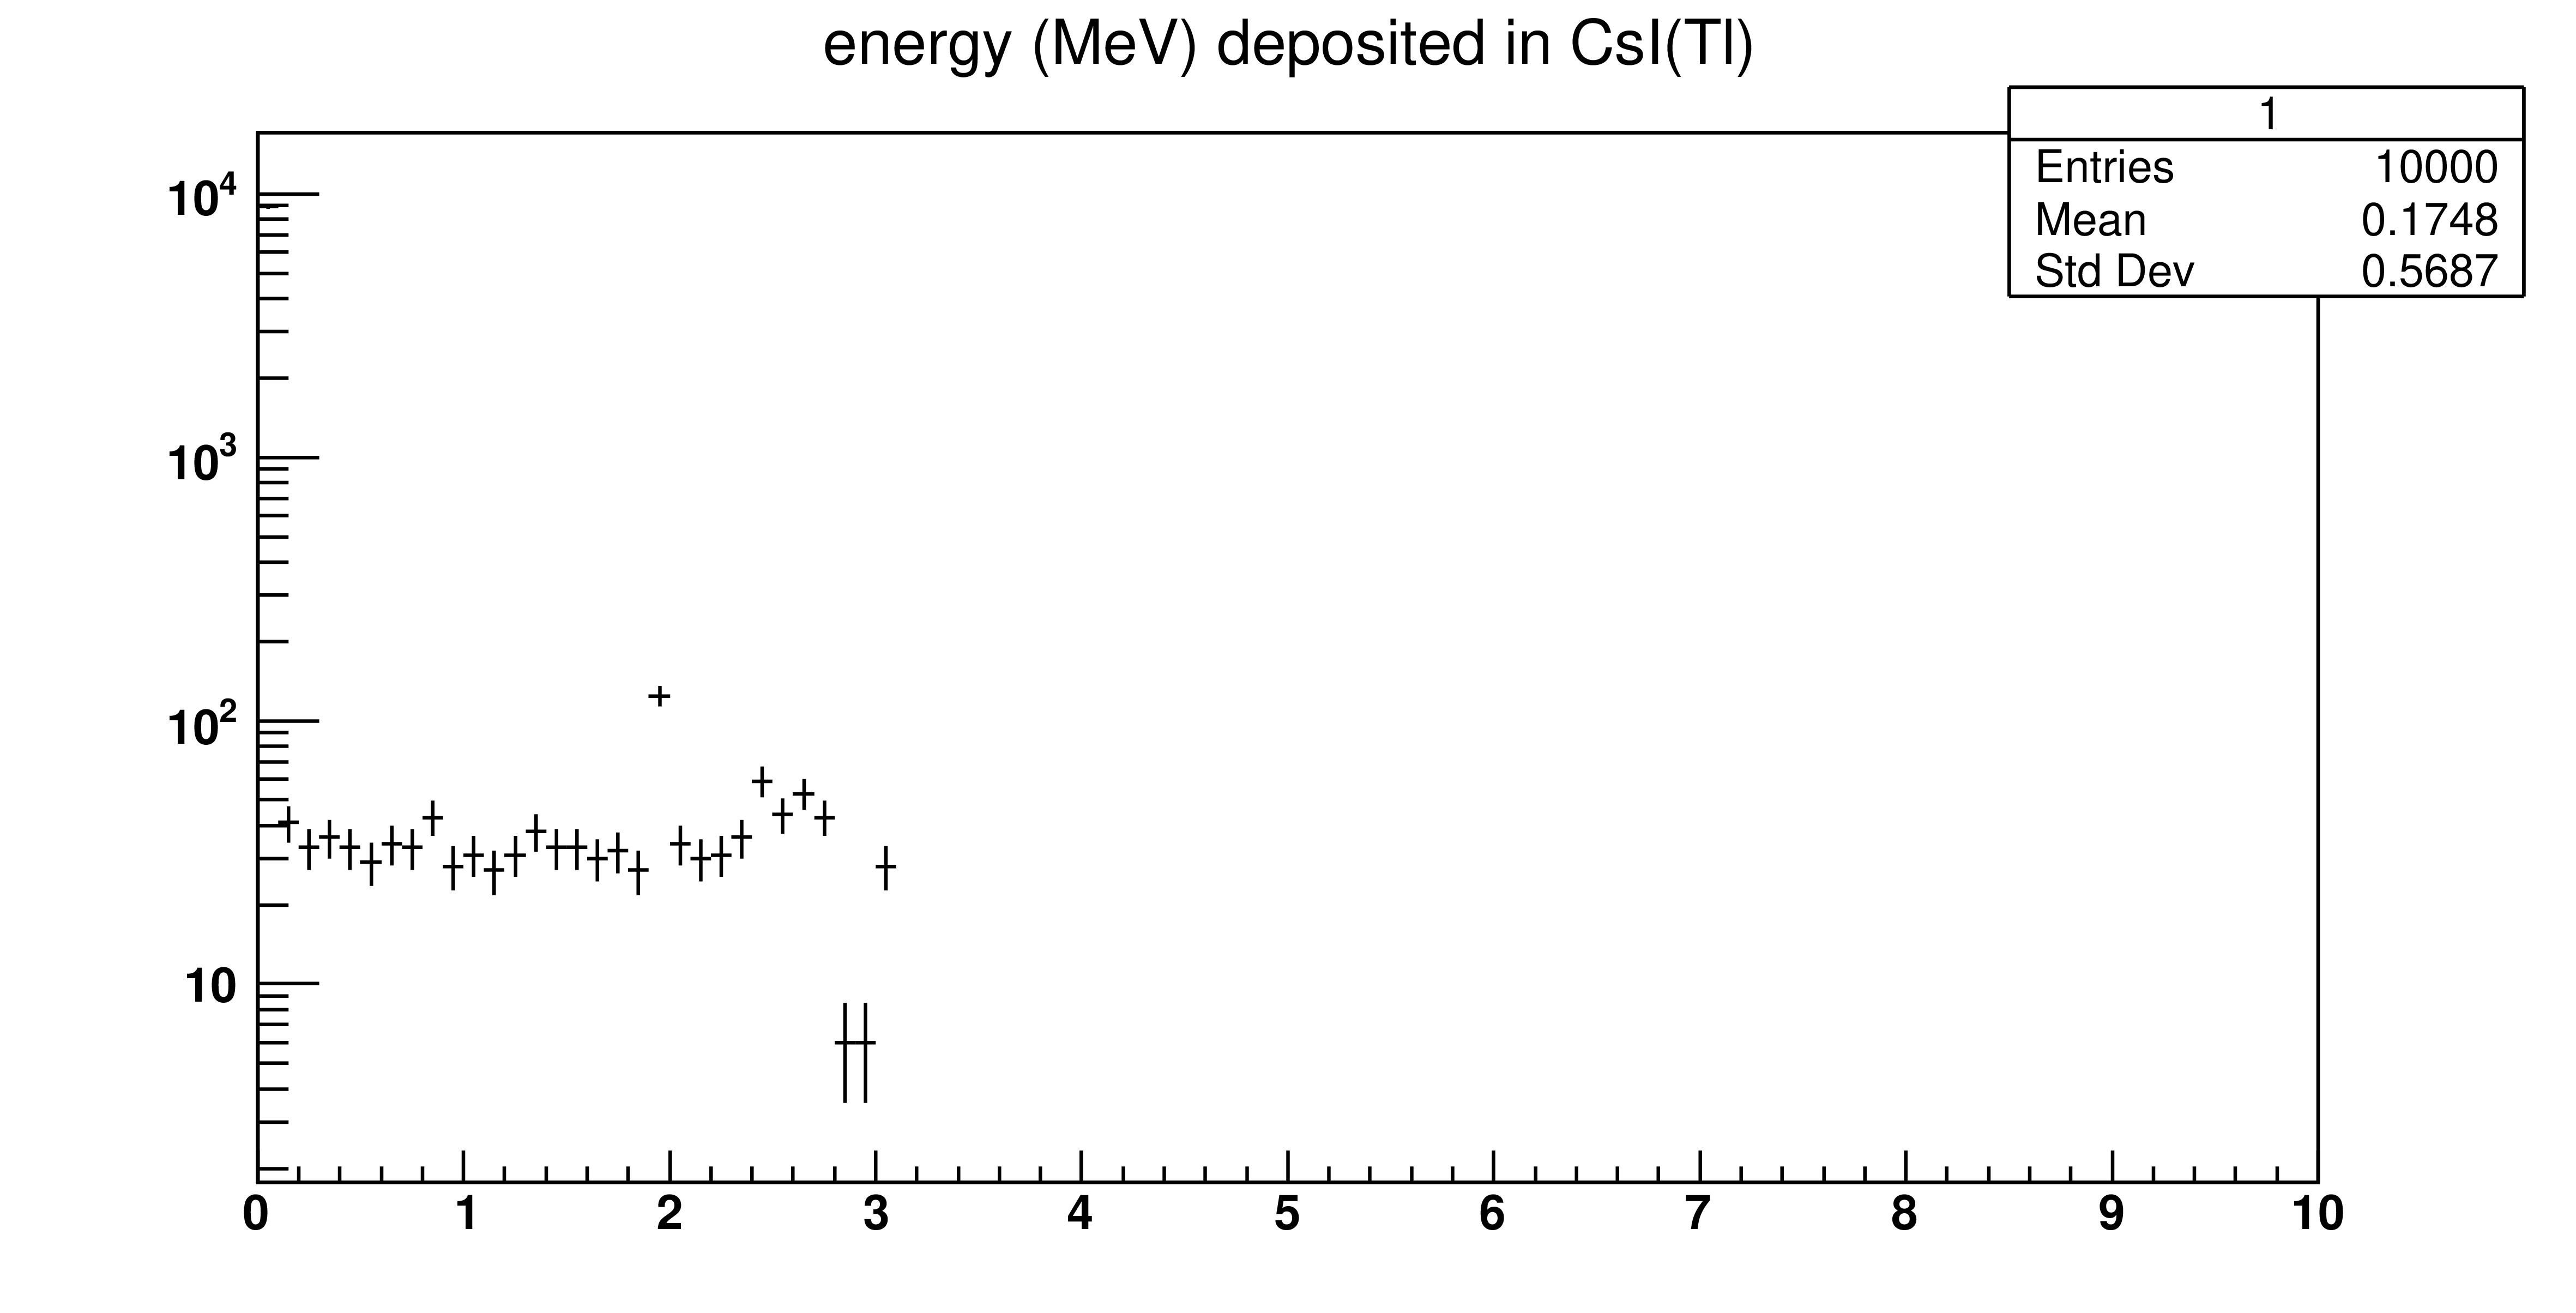
\includegraphics[width=\linewidth]{images/task1/CsI_3MeV.png}
  \caption{Deposited energy in CsI(Tl) at 3 MeV incident energy}
\end{subfigure}%
\begin{subfigure}{.5\textwidth}
  \centering
  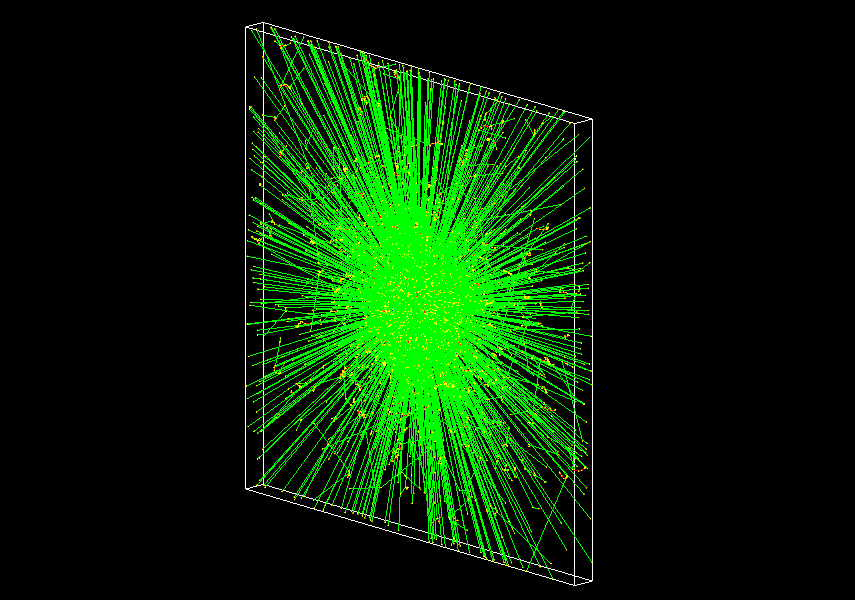
\includegraphics[width=\linewidth]{images/task1/CsI_3MeV_10000.png}
  \caption{Visualisation of the particle tracks}
\end{subfigure}
\caption{Results – CsI(Tl) – 3 MeV}
\end{figure}

\begin{figure}[H]
\centering
\begin{subfigure}{.5\textwidth}
  \centering
  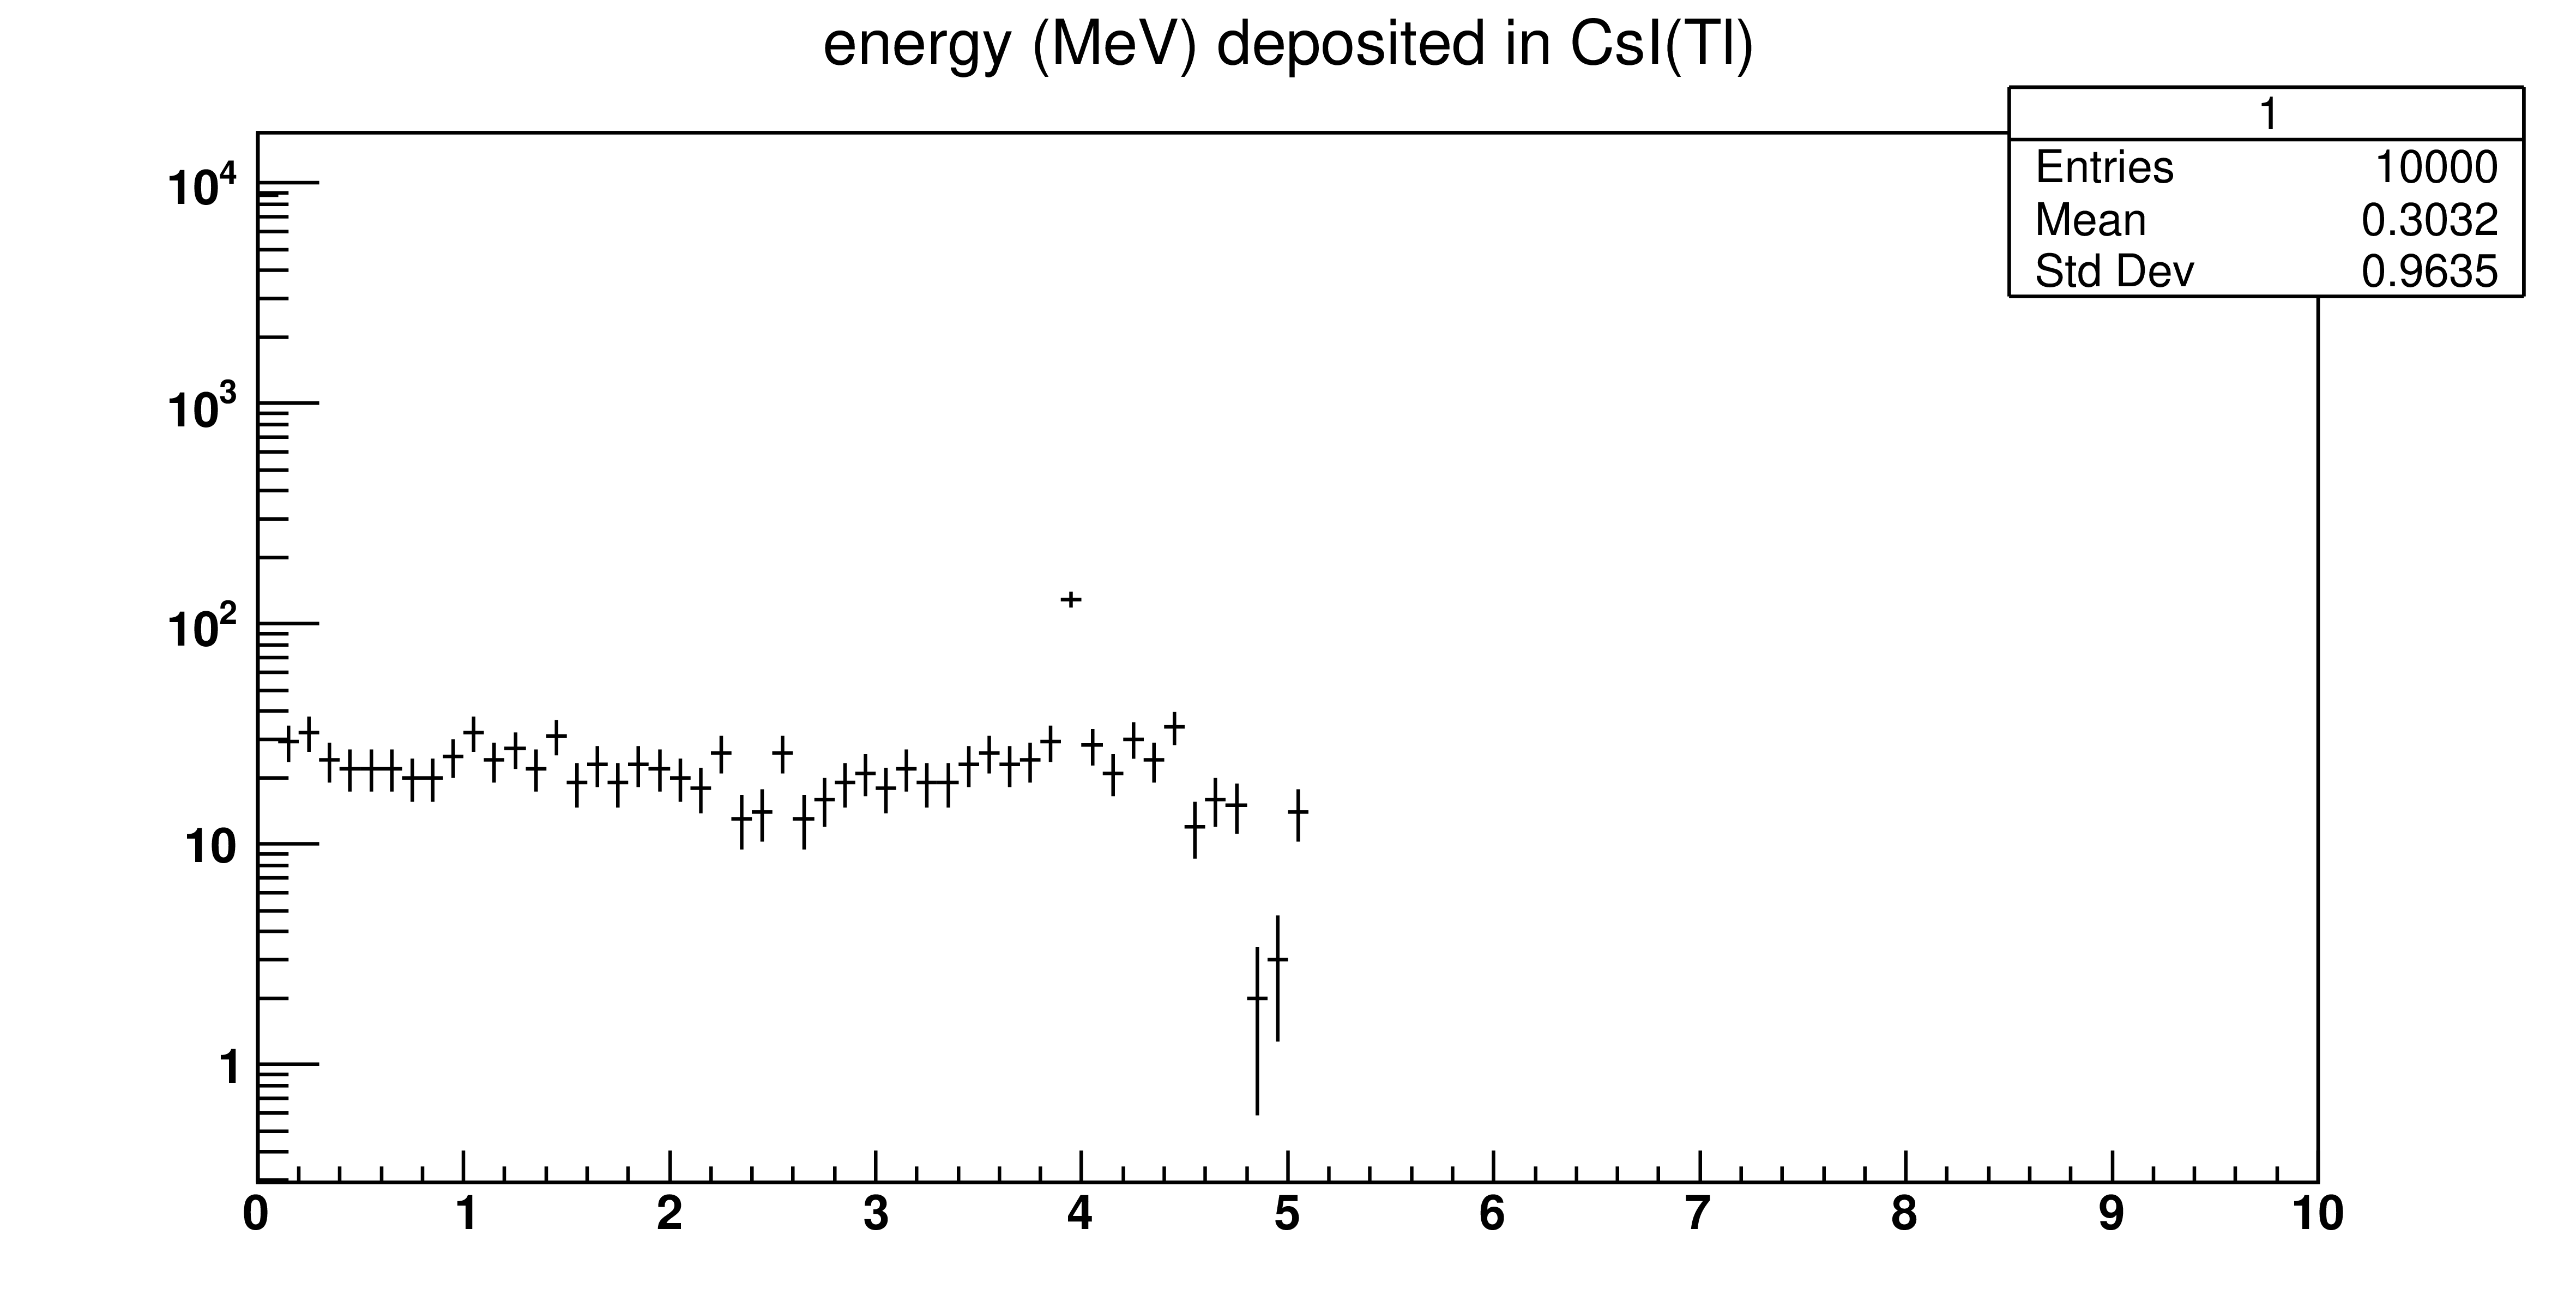
\includegraphics[width=\linewidth]{images/task1/CsI_5MeV.png}
  \caption{Deposited energy in CsI(Tl) at 5 MeV incident energy}
\end{subfigure}%
\begin{subfigure}{.5\textwidth}
  \centering
  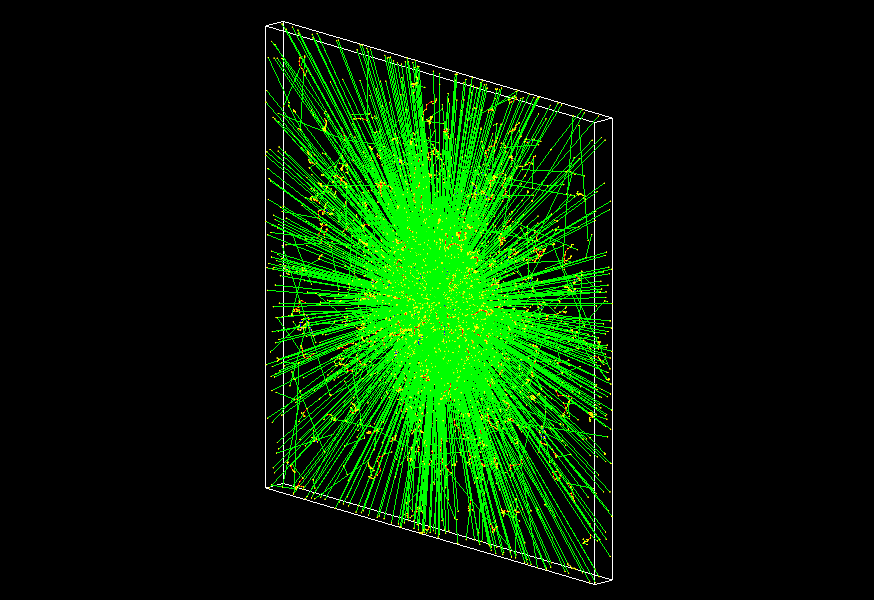
\includegraphics[width=\linewidth]{images/task1/CsI_5MeV_10000.png}
  \caption{Visualisation of the particle tracks}
\end{subfigure}
\caption{Results – CsI(Tl) – 5 MeV}
\end{figure}

\begin{figure}[H]
\centering
\begin{subfigure}{.5\textwidth}
  \centering
  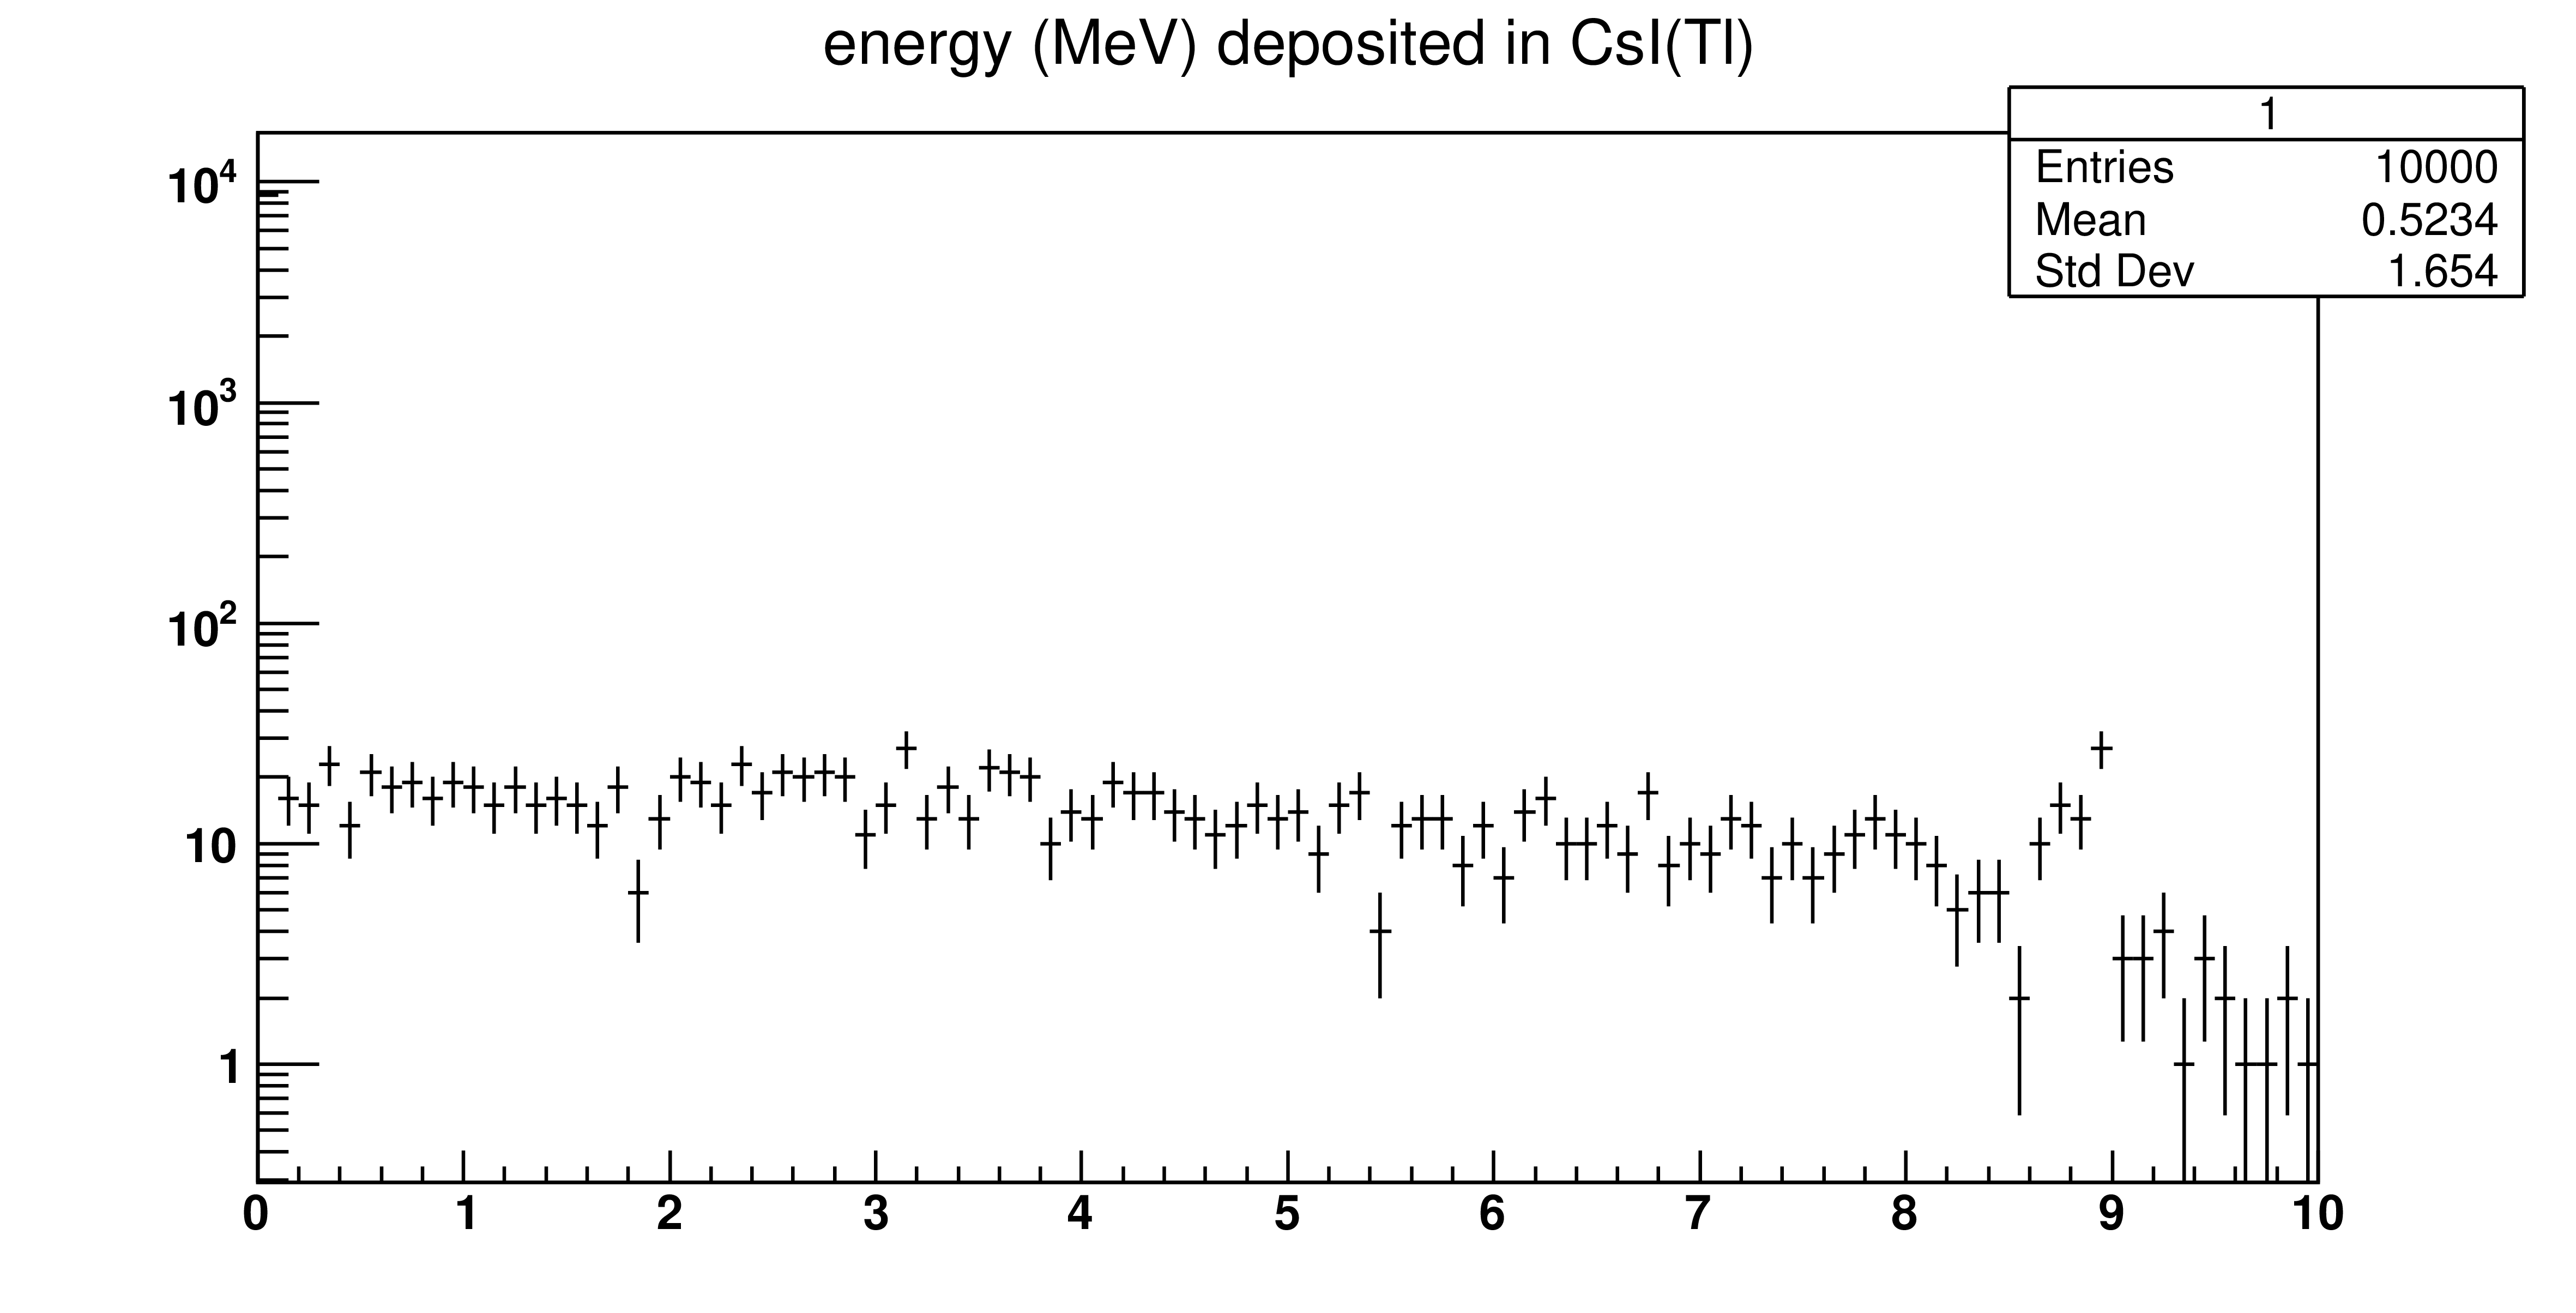
\includegraphics[width=\linewidth]{images/task1/CsI_10MeV.png}
  \caption{Deposited energy in CsI(Tl) at 10 MeV incident energy}  % chktex 36
\end{subfigure}%
\begin{subfigure}{.5\textwidth}
  \centering
  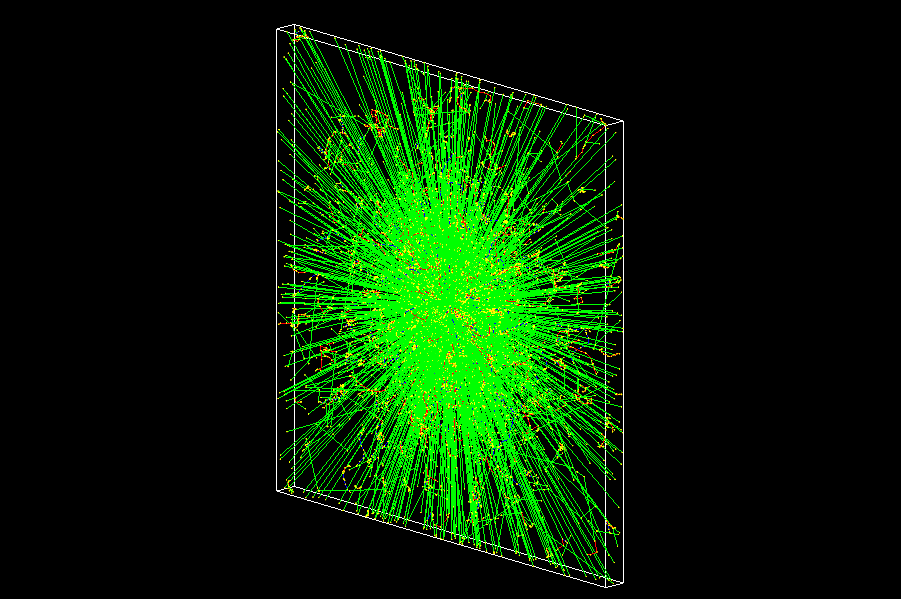
\includegraphics[width=\linewidth]{images/task1/CsI_10MeV_10000.png}
  \caption{Visualisation of the particle tracksy}
\end{subfigure}
\caption{Results – CsI(Tl) – 10 MeV}  % chktex 8
\end{figure}


\subsubsection{BGO}
\begin{figure}[H]
\centering
\begin{subfigure}{.5\textwidth}
  \centering
  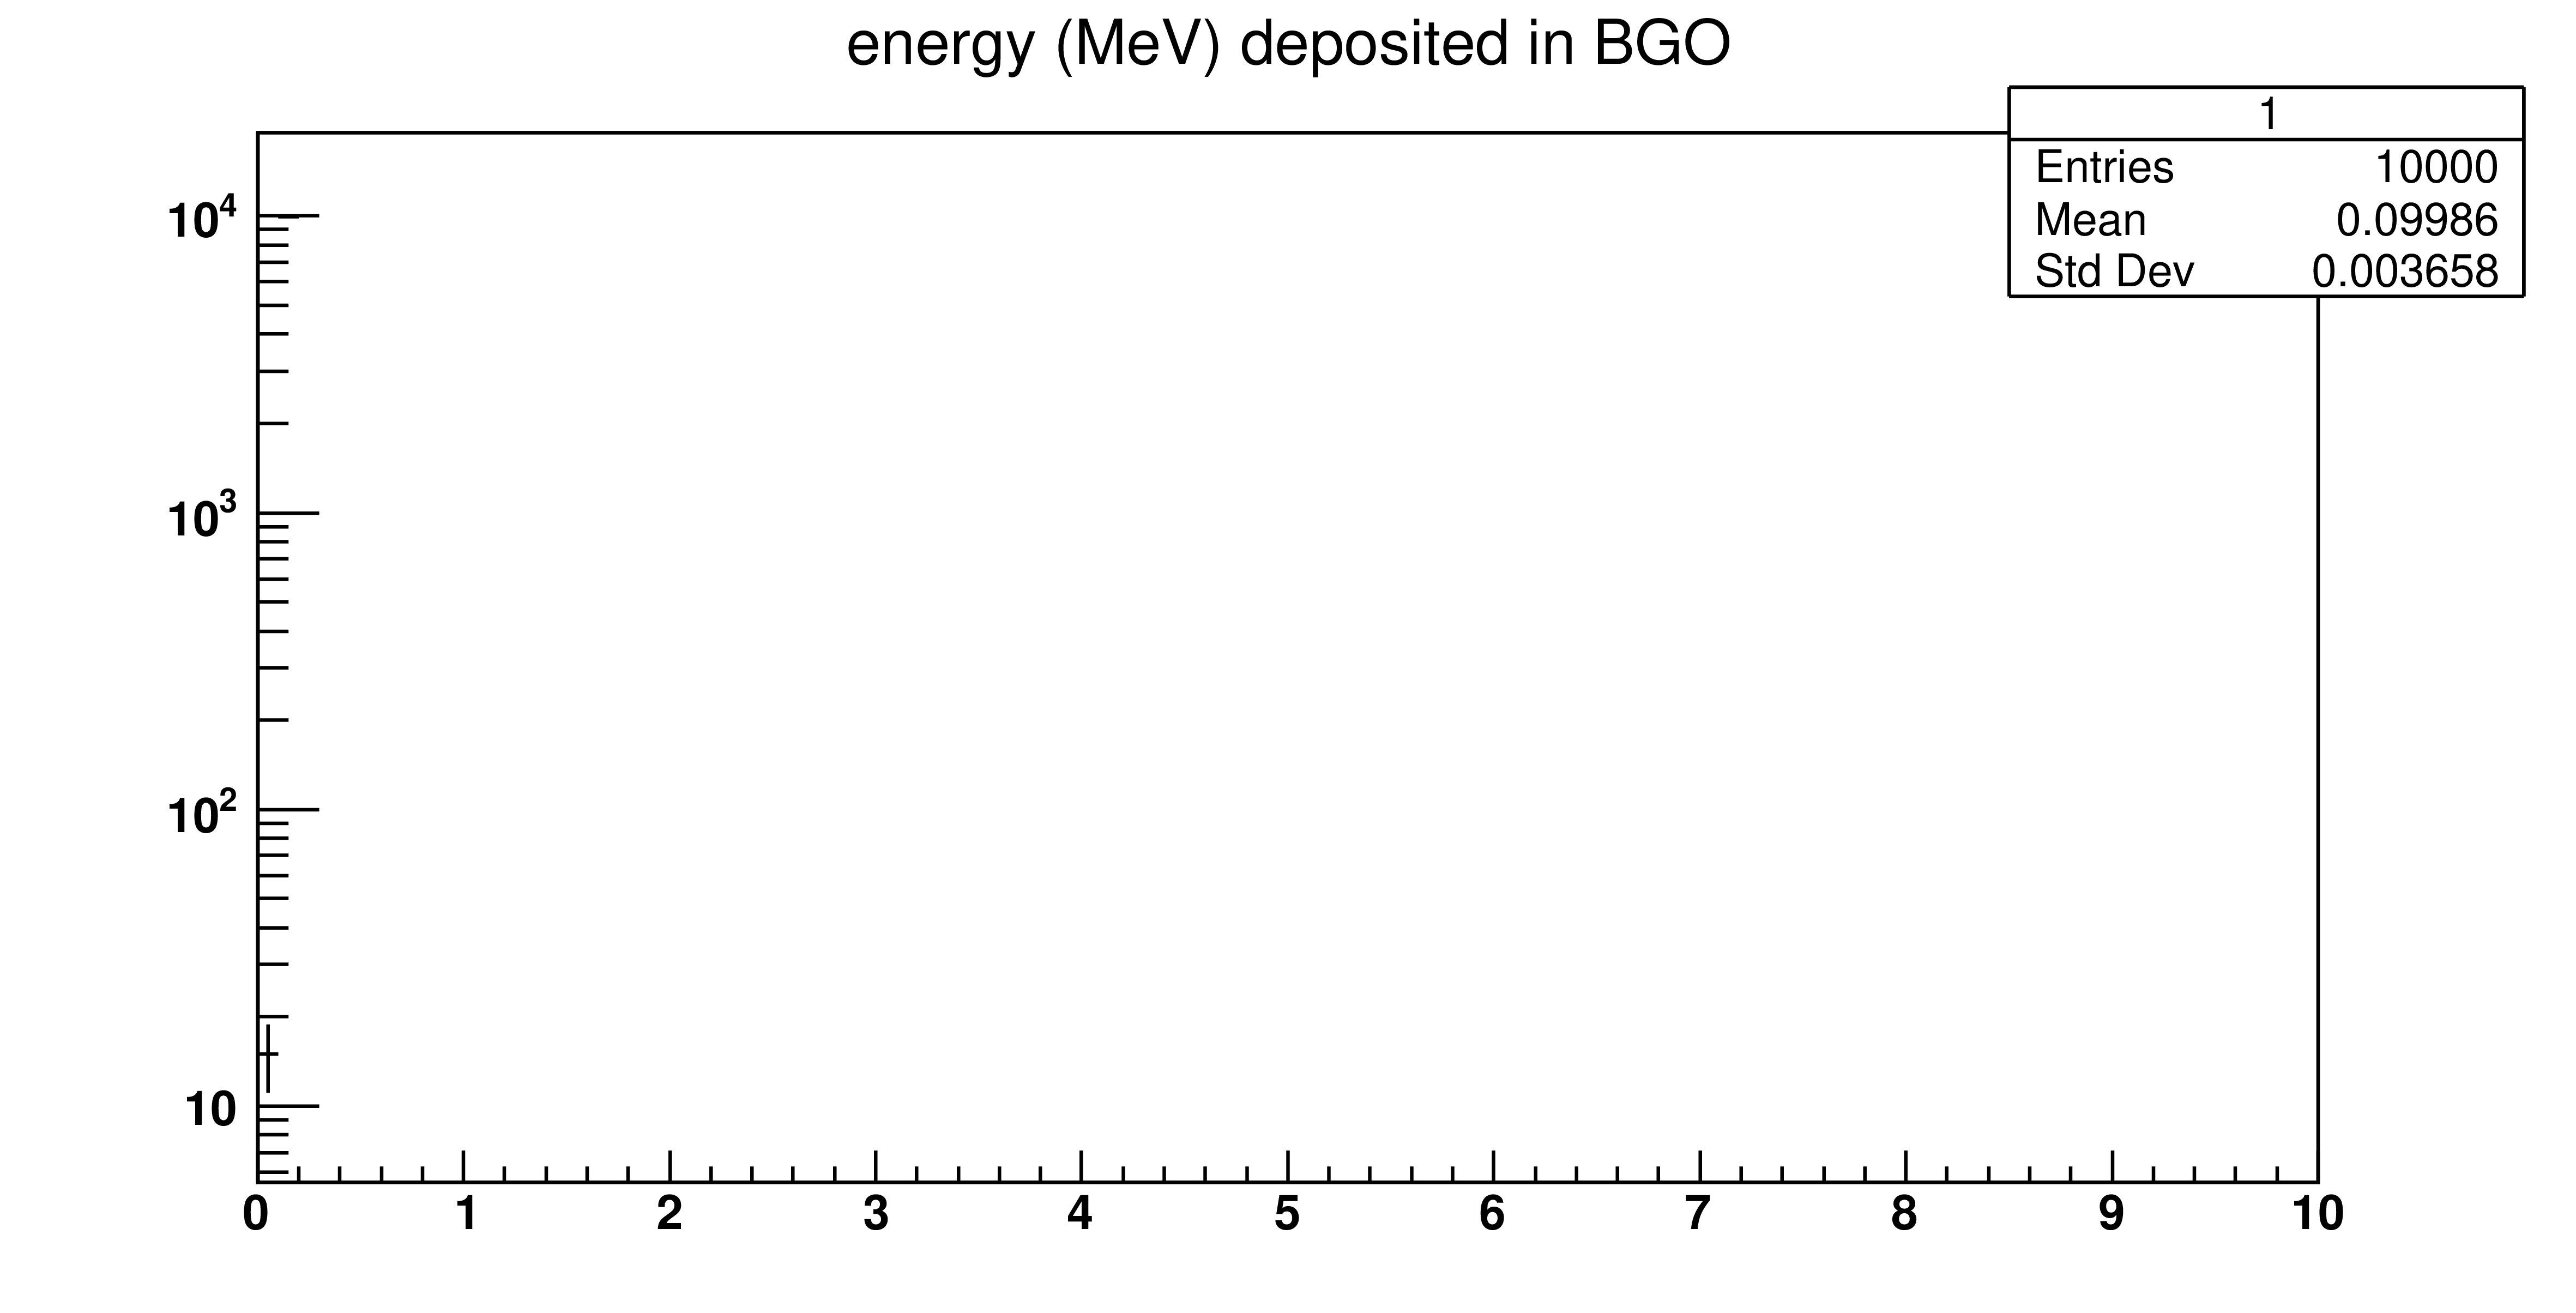
\includegraphics[width=\linewidth]{images/task1/BGO_01MeV.png}
  \caption{Deposited energy in BGO at 0.1 MeV incident energy}
\end{subfigure}%
\begin{subfigure}{.5\textwidth}
  \centering
  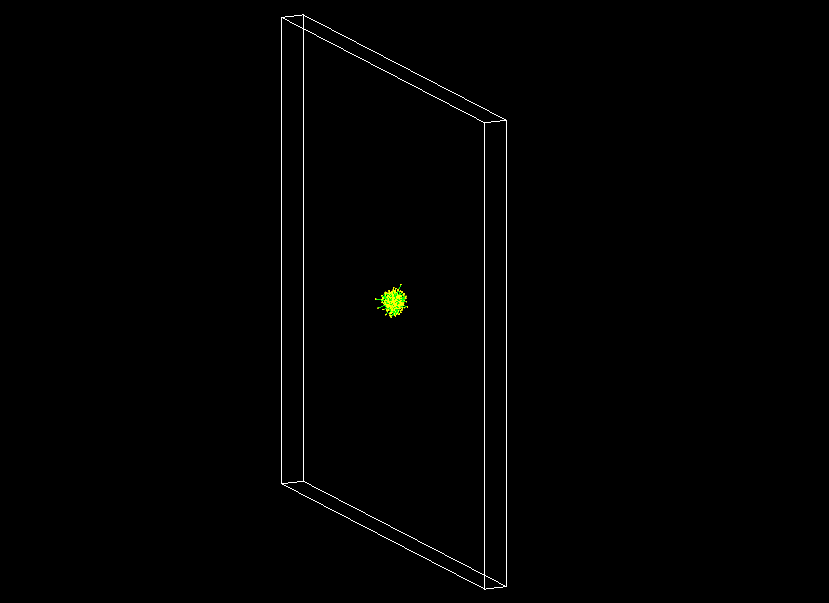
\includegraphics[width=\linewidth]{images/task1/BGO_01MeV_10000.png}
  \caption{Visualisation of the particle tracks}
\end{subfigure}
\caption{Results – BGO – 0.1 MeV}
\end{figure}

\begin{figure}[H]
\centering
\begin{subfigure}{.5\textwidth}
  \centering
  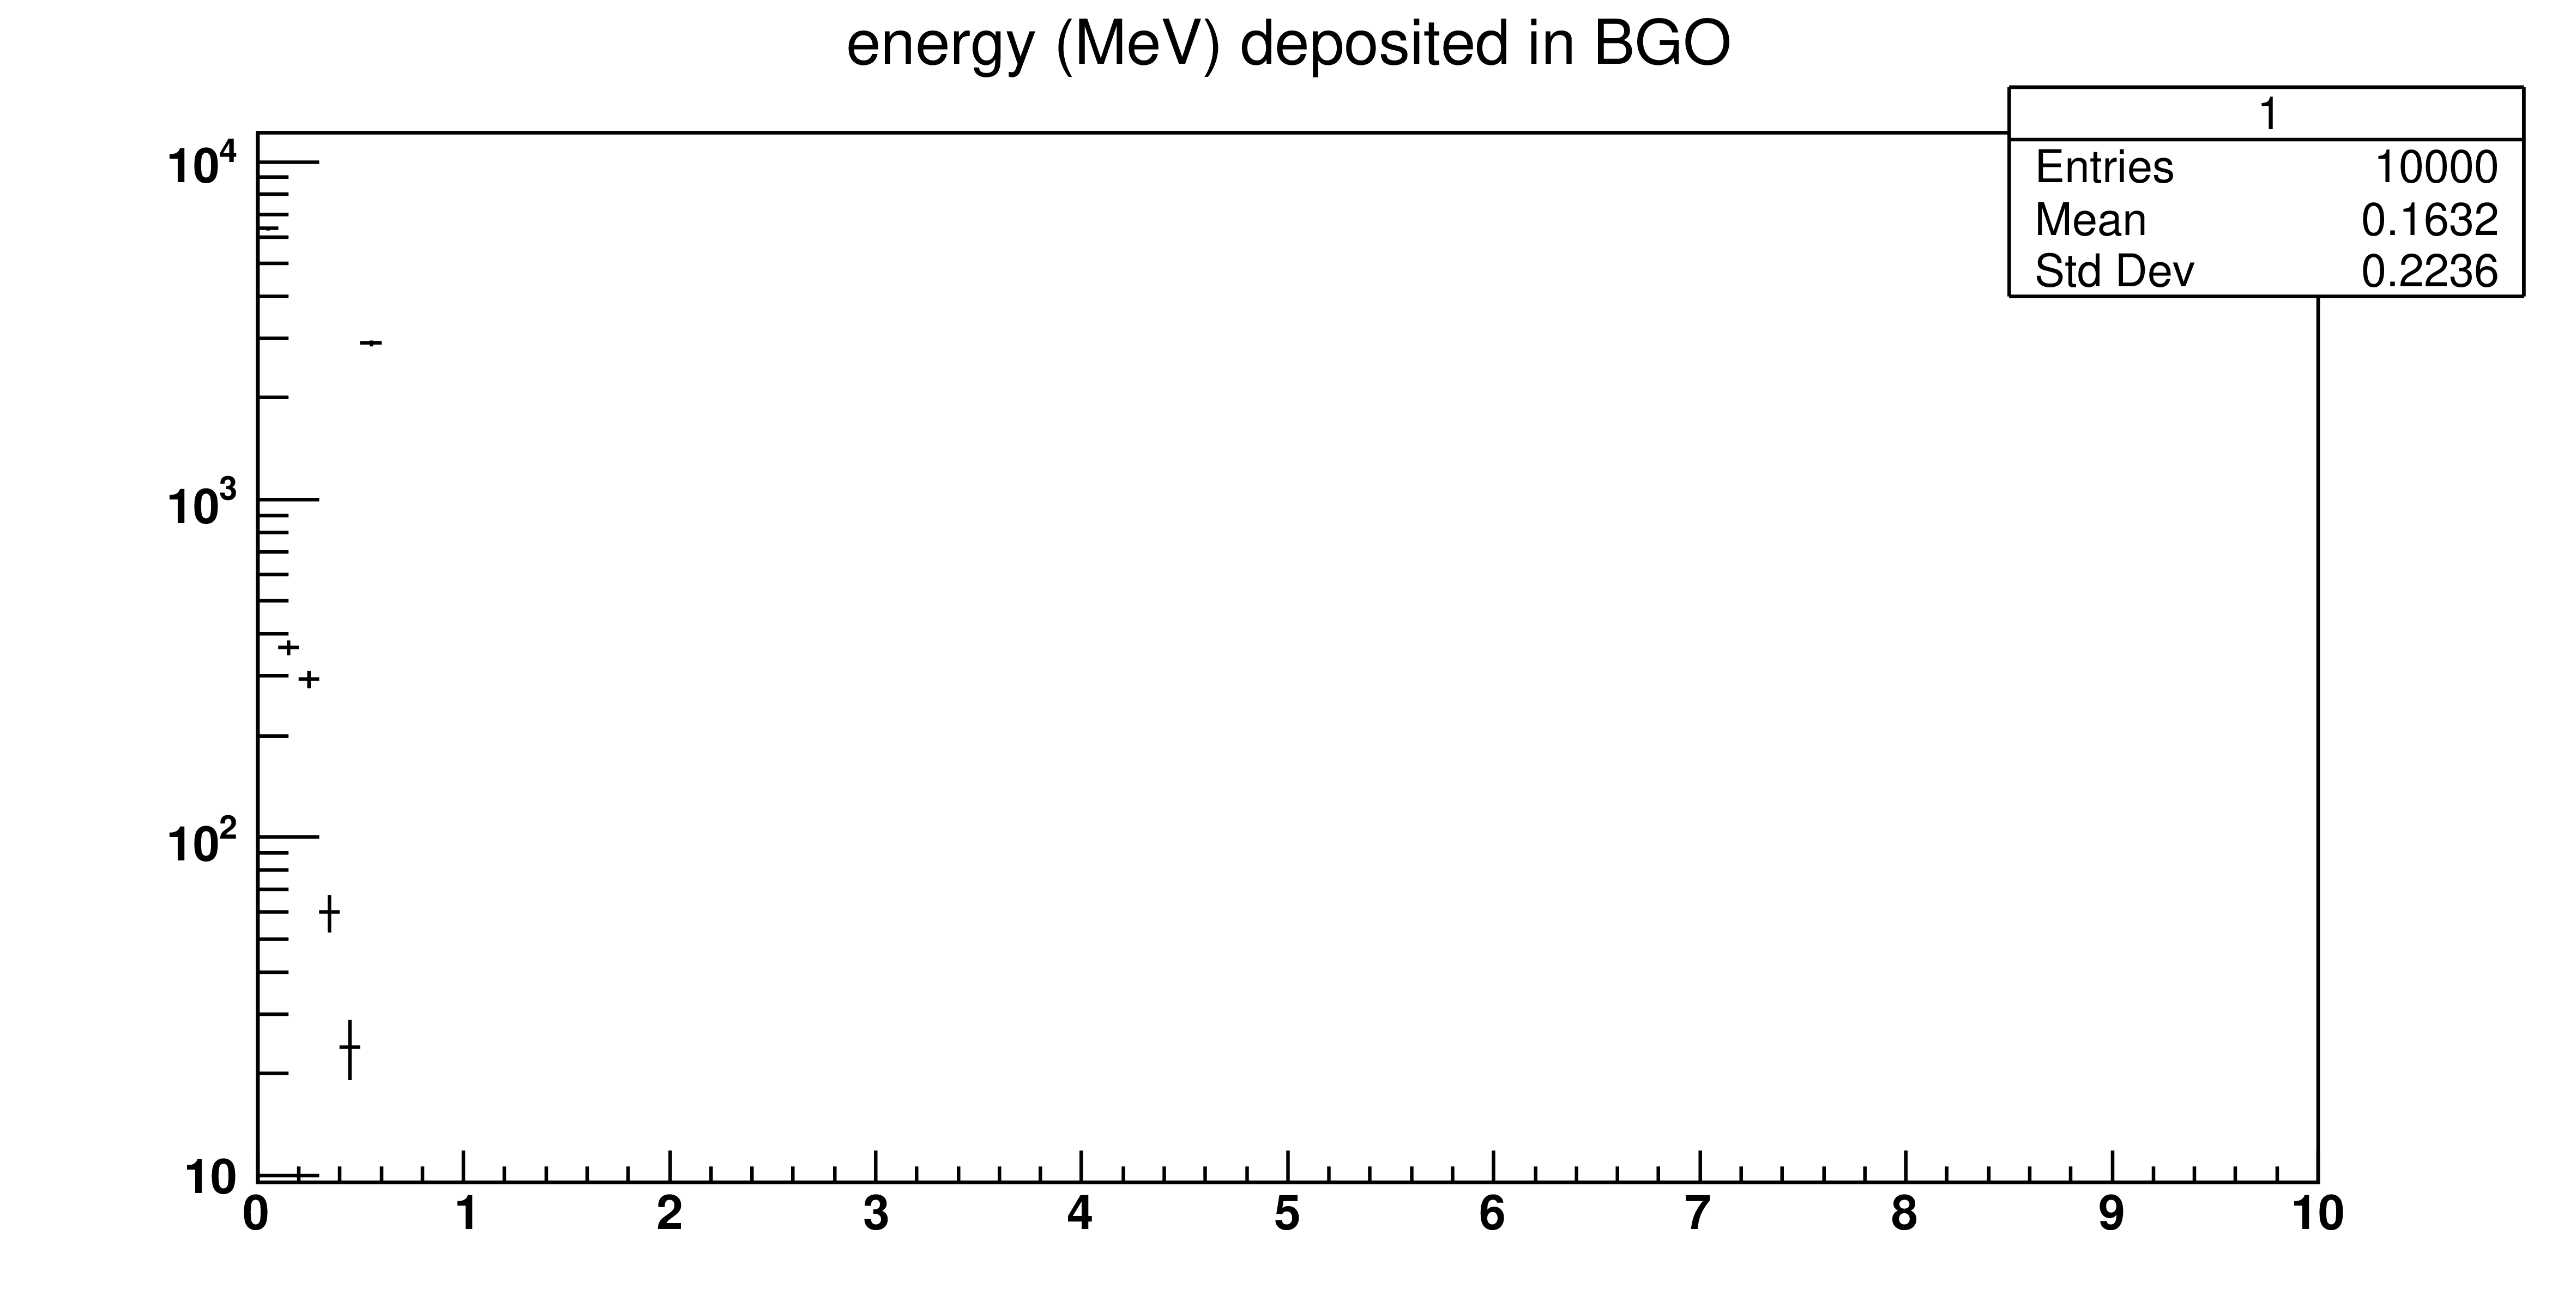
\includegraphics[width=\linewidth]{images/task1/BGO_05MeV.png}
  \caption{Deposited energy in BGO at 0.5 MeV incident energy}
\end{subfigure}%
\begin{subfigure}{.5\textwidth}
  \centering
  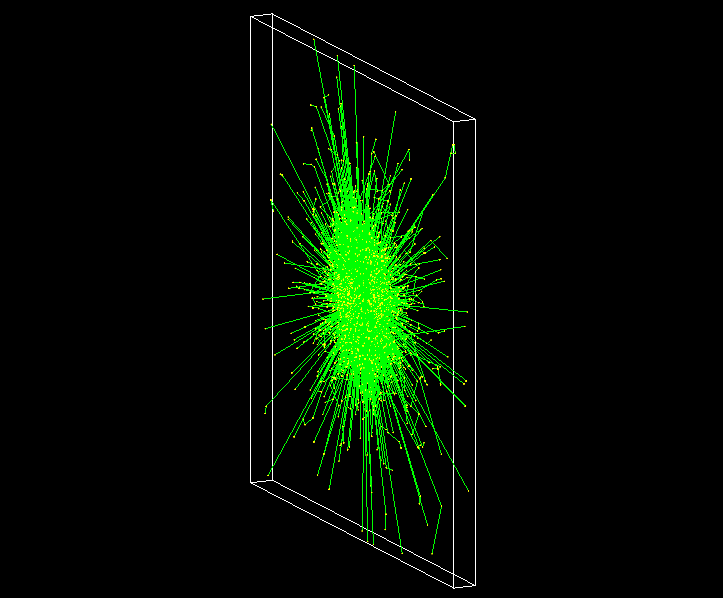
\includegraphics[width=\linewidth]{images/task1/BGO_05MeV_10000.png}
  \caption{Visualisation of the particle tracks}
\end{subfigure}
\caption{Results – BGO – 0.5 MeV}
\end{figure}

\begin{figure}[H]
\centering
\begin{subfigure}{.5\textwidth}
  \centering
  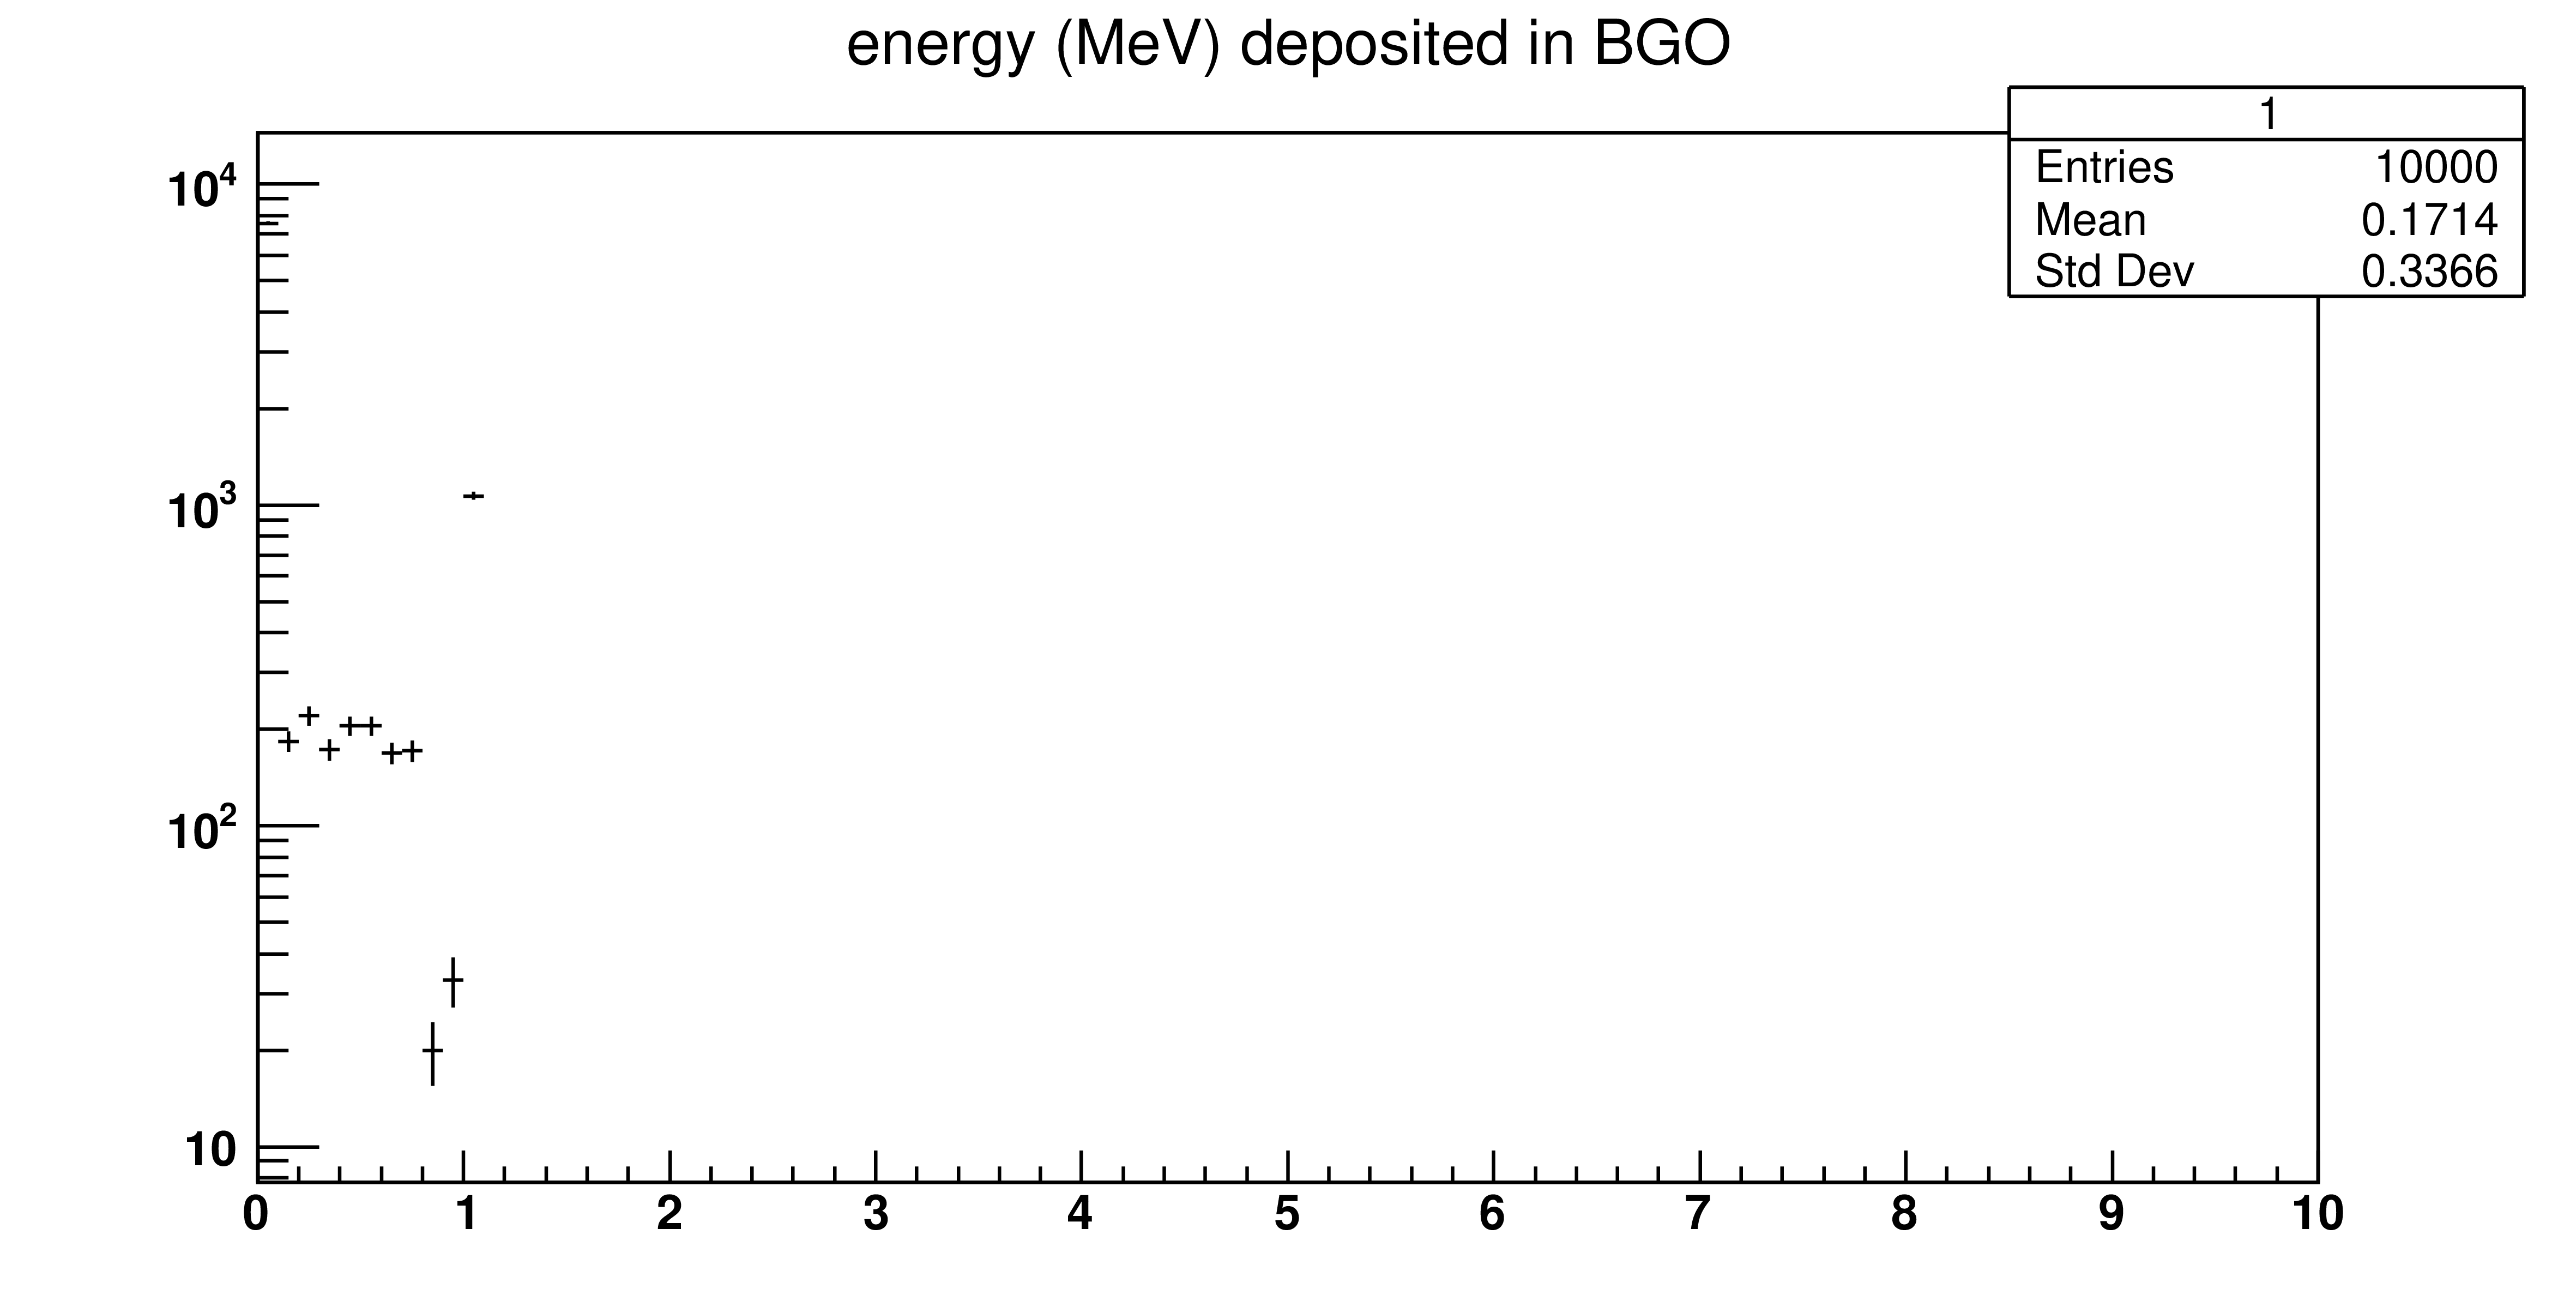
\includegraphics[width=\linewidth]{images/task1/BGO_1MeV.png}
  \caption{Deposited energy in BGO at 1 MeV incident energy}
\end{subfigure}%
\begin{subfigure}{.5\textwidth}
  \centering
  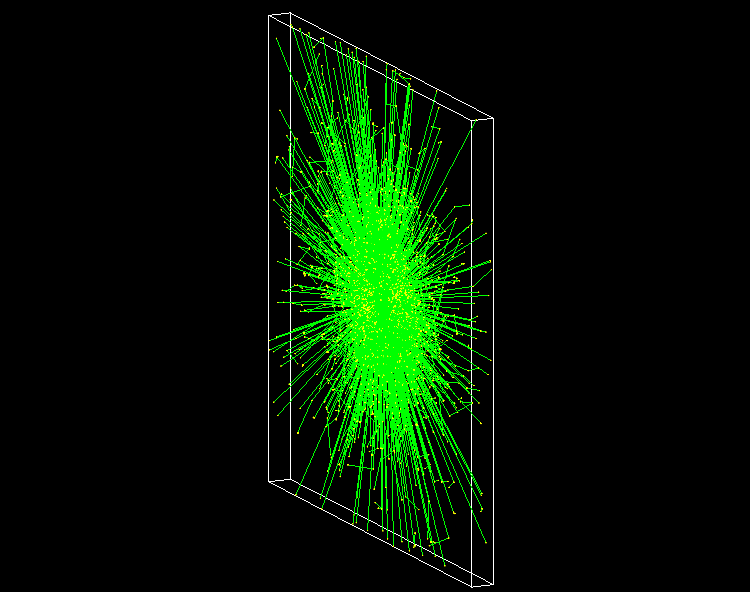
\includegraphics[width=\linewidth]{images/task1/BGO_1MeV_10000.png}
  \caption{Visualisation of the particle tracks}
\end{subfigure}
\caption{Results – BGO – 1 MeV}
\end{figure}

\begin{figure}[H]
\centering
\begin{subfigure}{.5\textwidth}
  \centering
  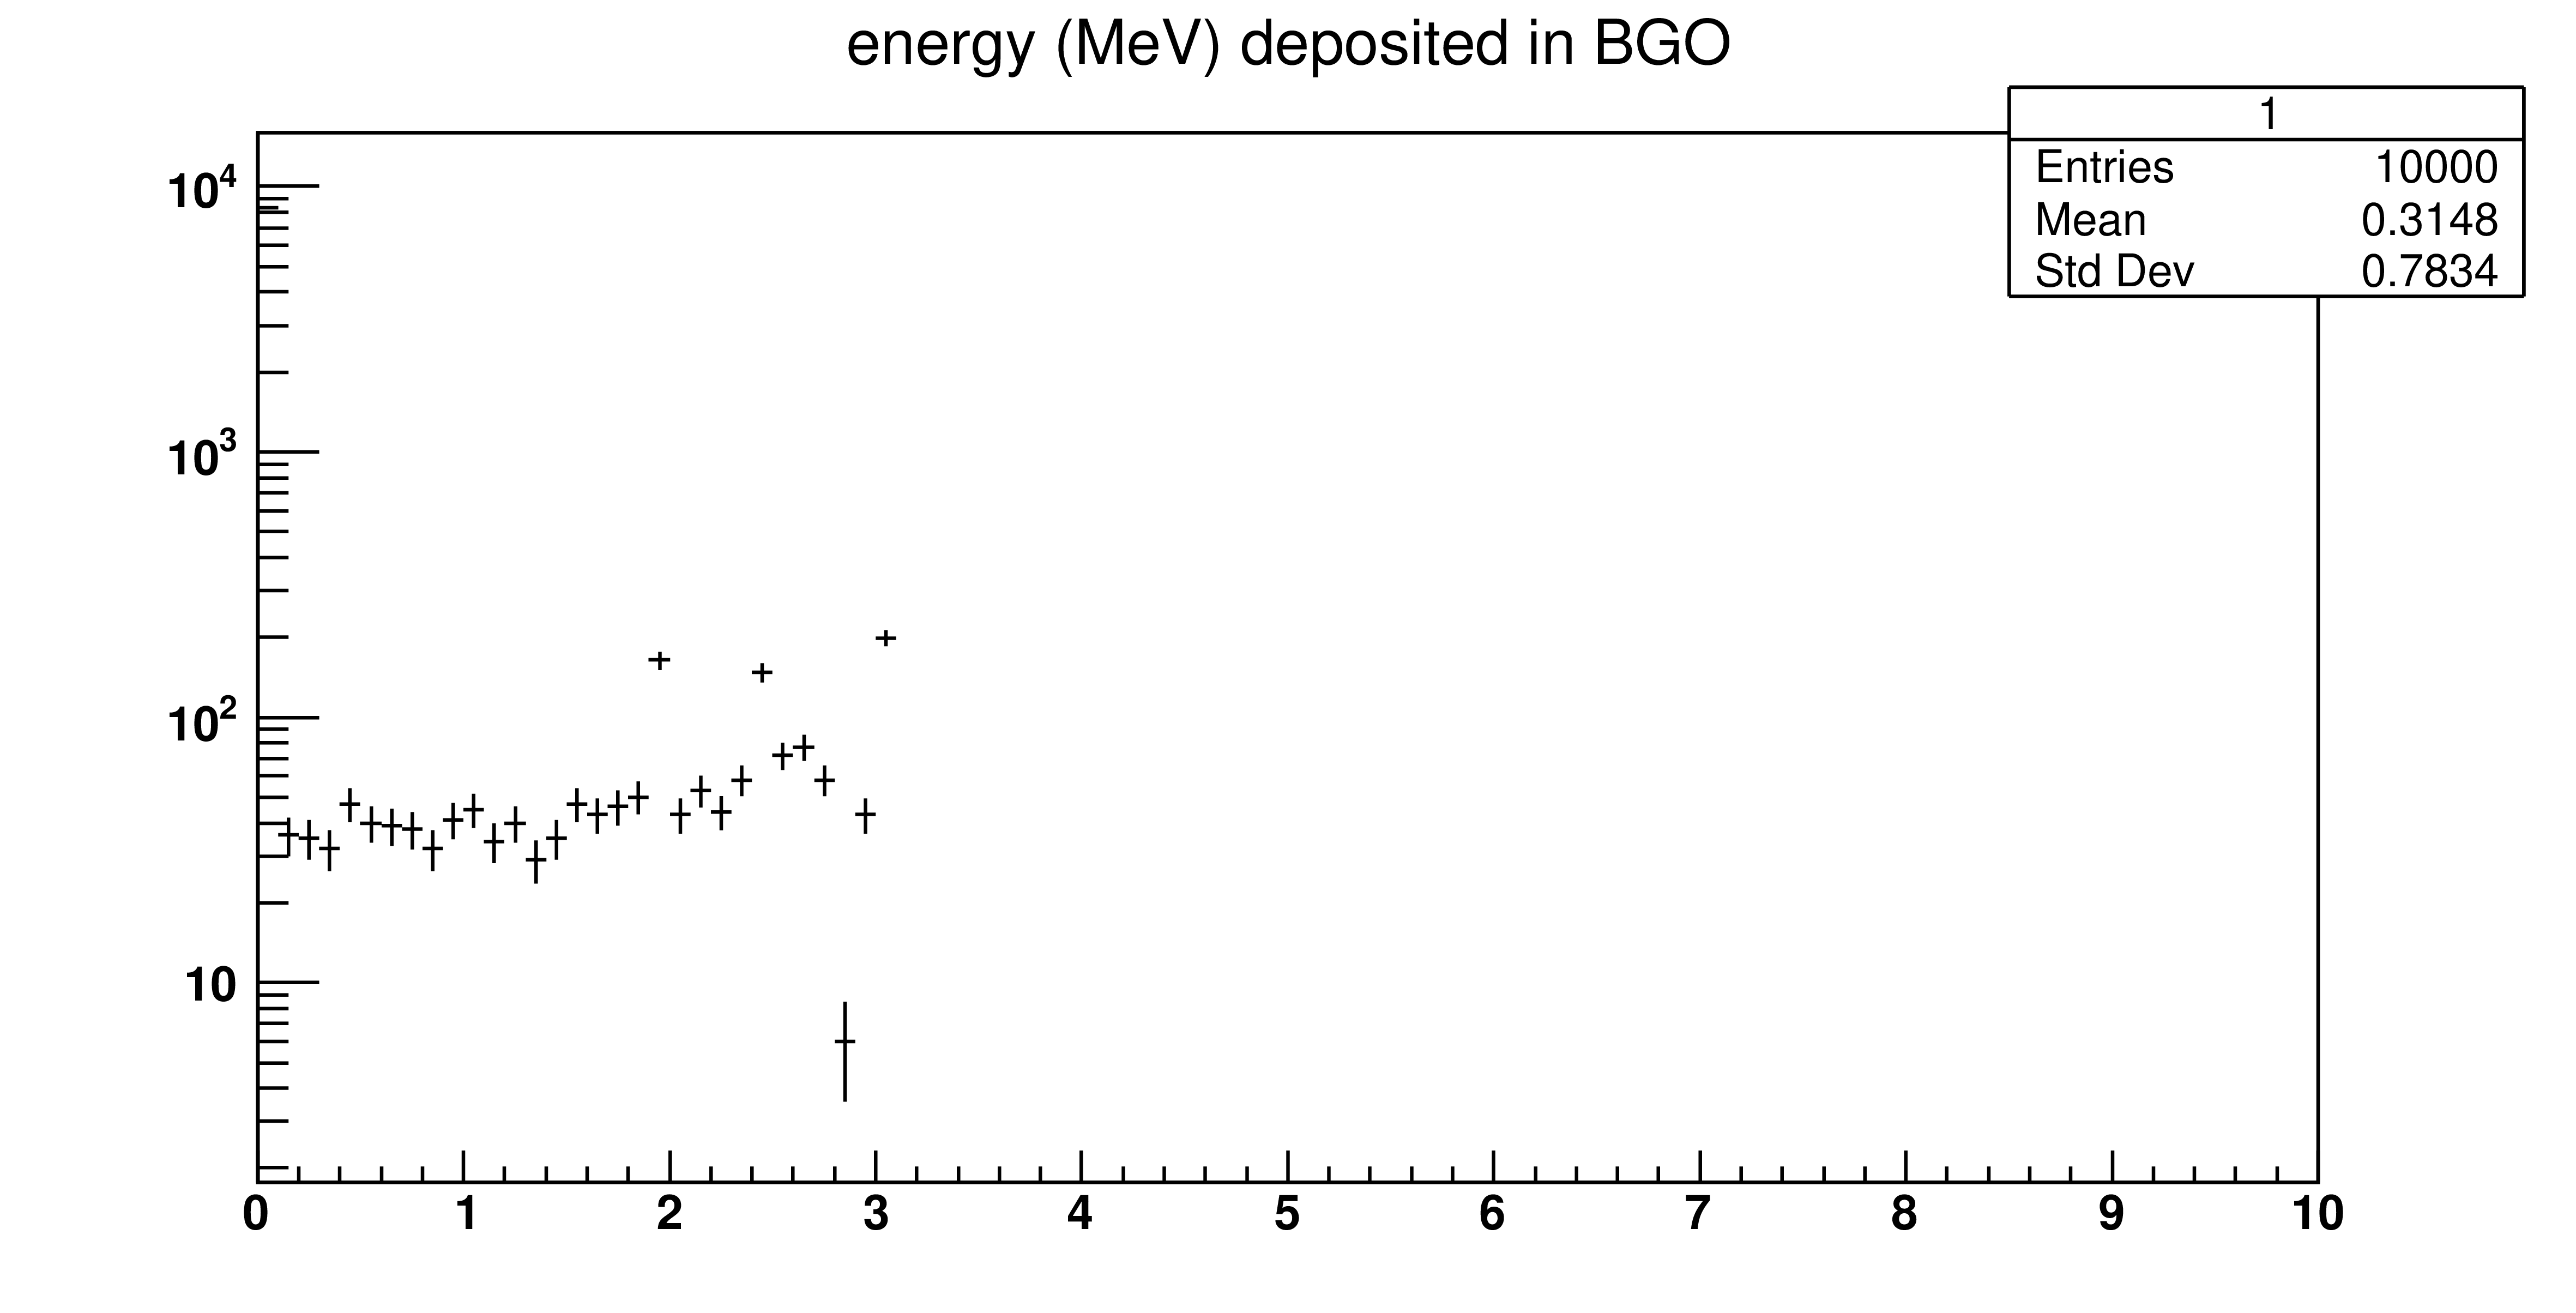
\includegraphics[width=\linewidth]{images/task1/BGO_3MeV.png}
  \caption{Deposited energy in BGO at 3 MeV incident energy}
\end{subfigure}%
\begin{subfigure}{.5\textwidth}
  \centering
  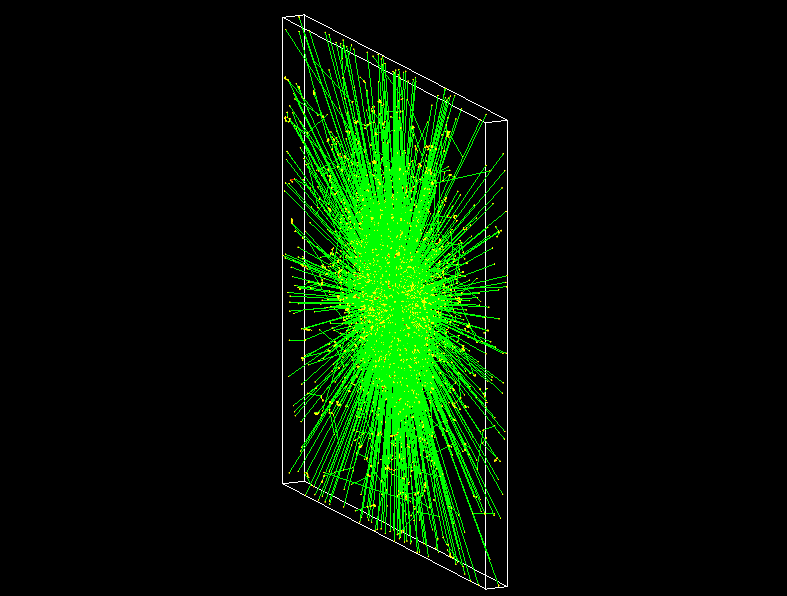
\includegraphics[width=\linewidth]{images/task1/BGO_3MeV_10000.png}
  \caption{Visualisation of the particle tracks}
\end{subfigure}
\caption{Results – BGO – 3 MeV}
\end{figure}

\begin{figure}[H]
\centering
\begin{subfigure}{.5\textwidth}
  \centering
  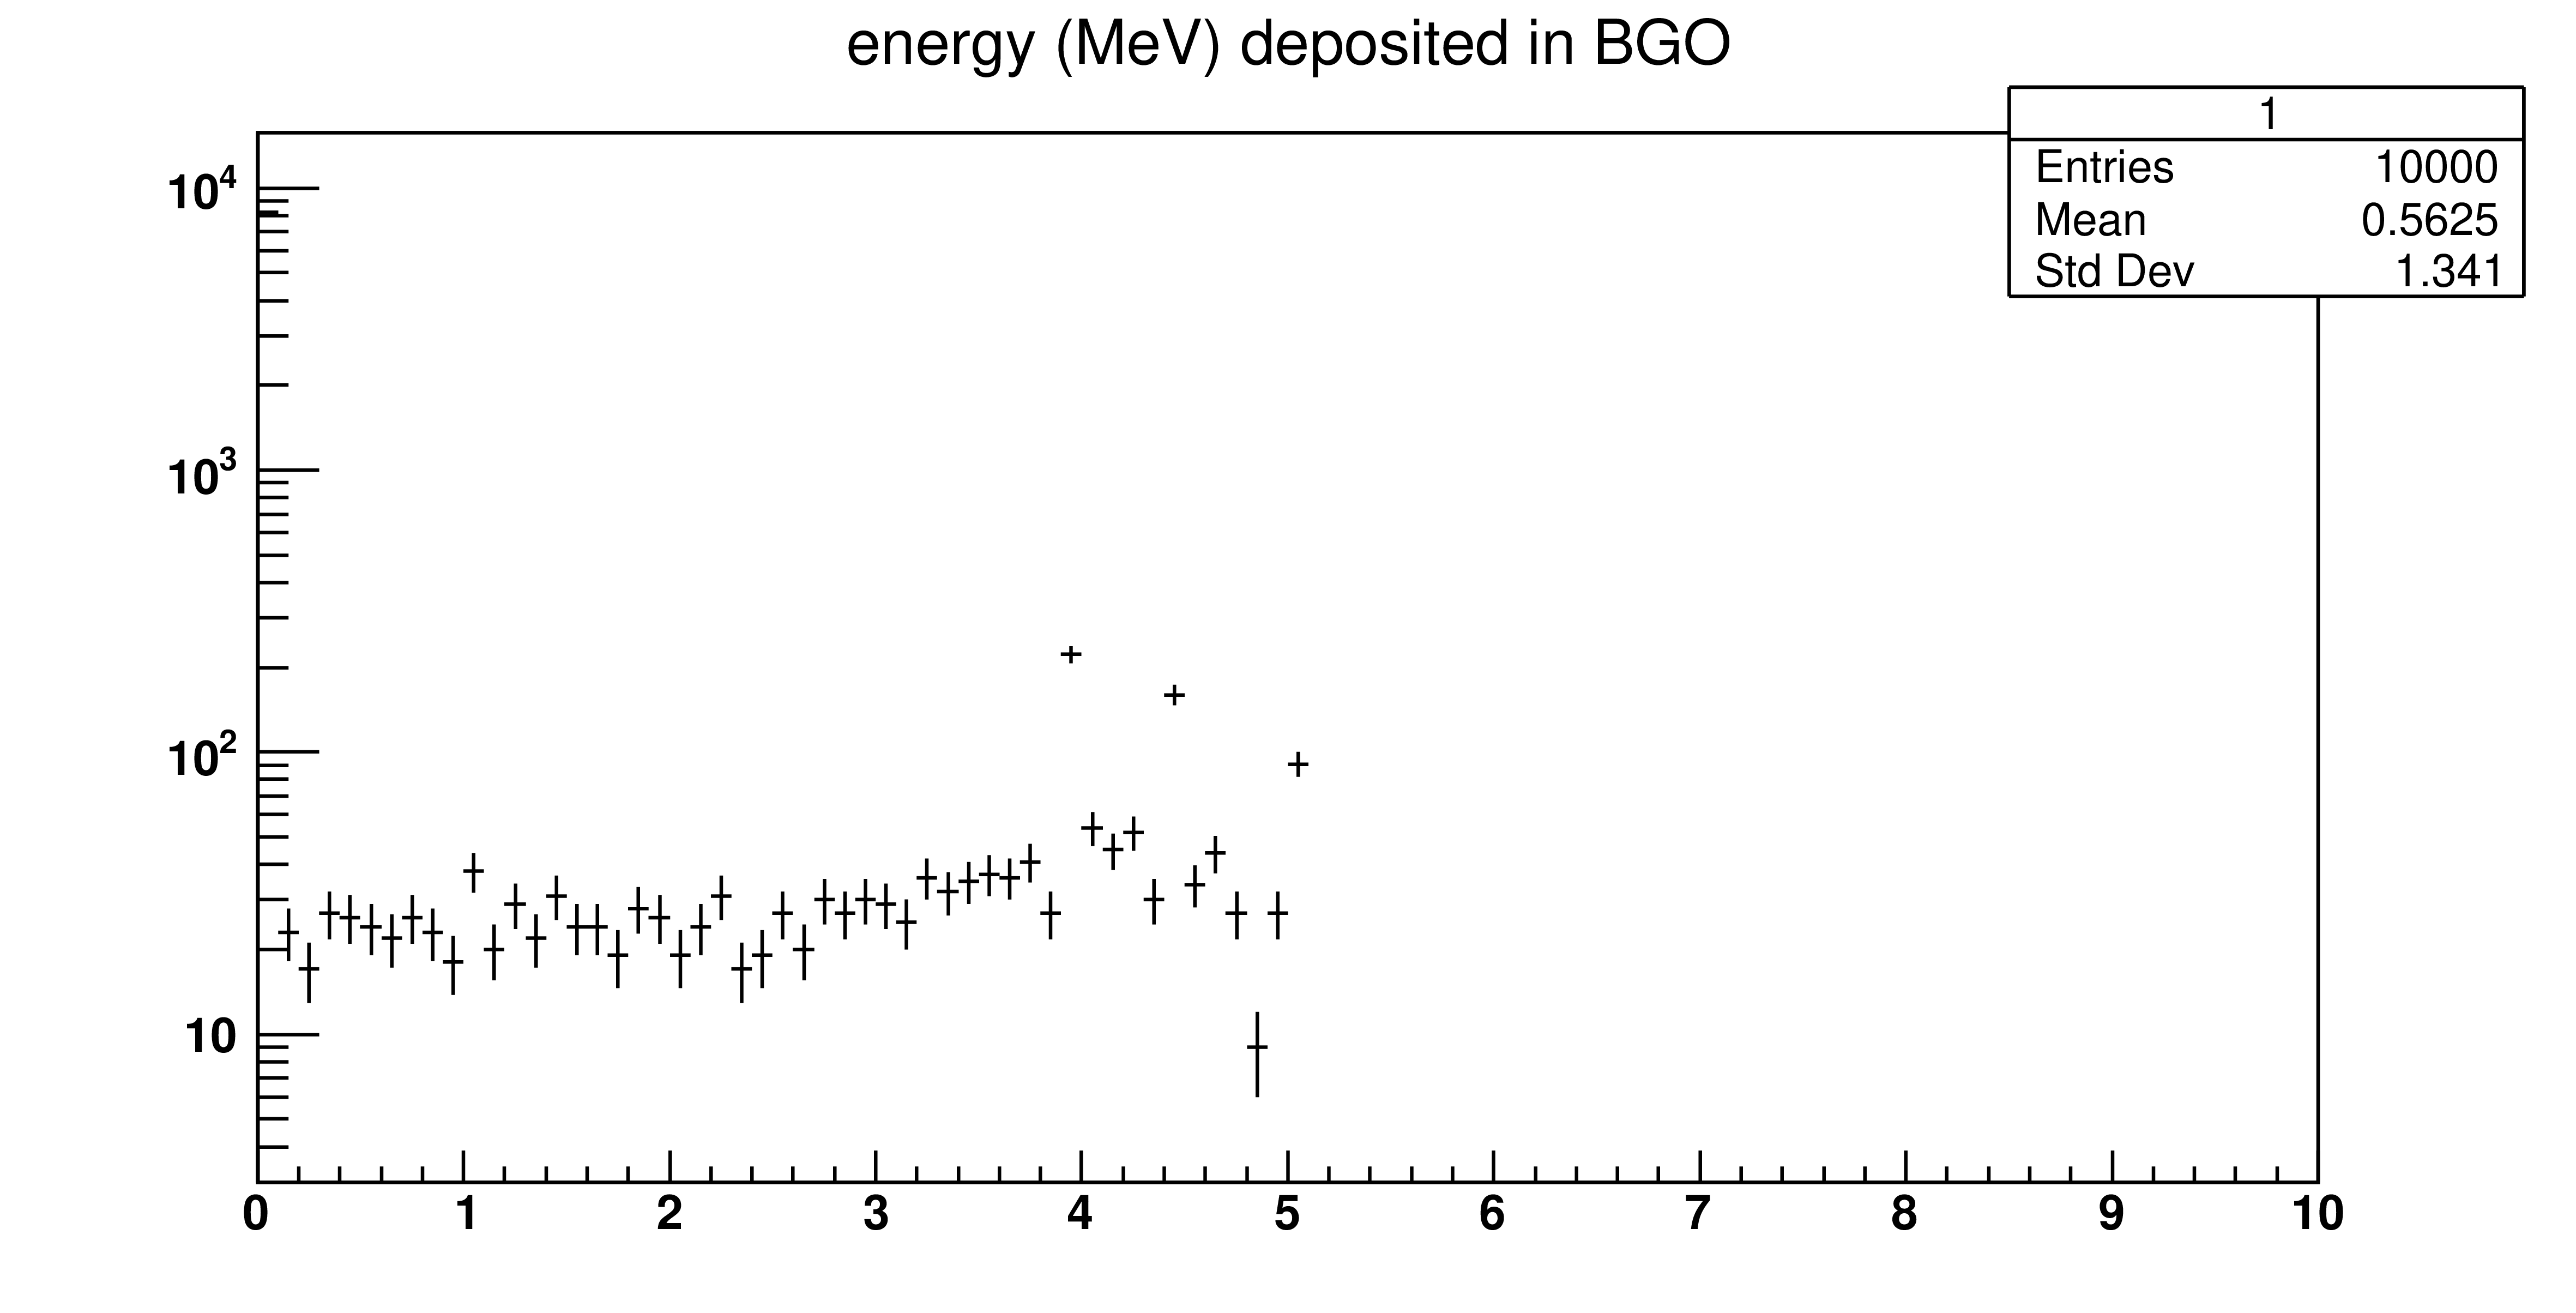
\includegraphics[width=\linewidth]{images/task1/BGO_5MeV.png}
  \caption{Deposited energy in BGO at 5 MeV incident energy}
\end{subfigure}%
\begin{subfigure}{.5\textwidth}
  \centering
  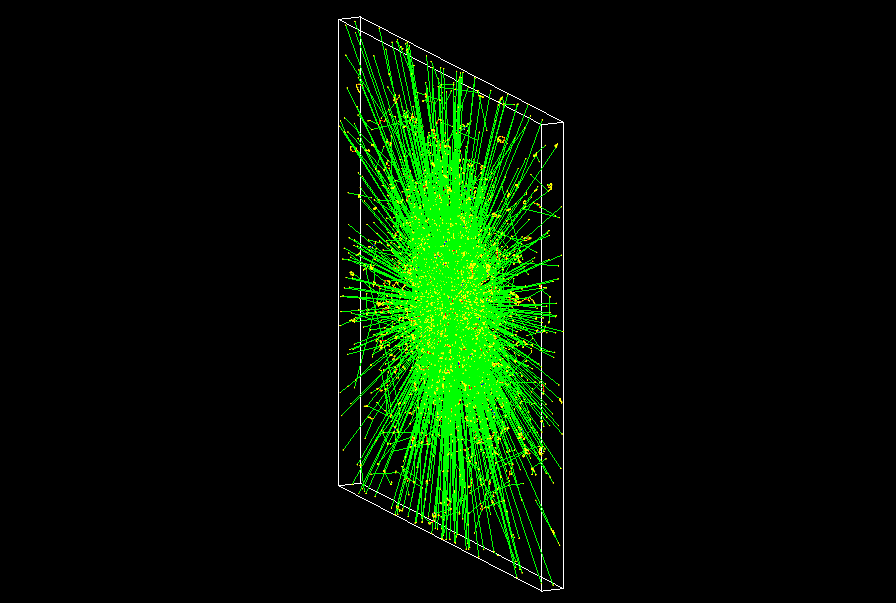
\includegraphics[width=\linewidth]{images/task1/BGO_5MeV_10000.png}
  \caption{Visualisation of the particle tracks}
\end{subfigure}
\caption{Results – BGO – 5 MeV}
\end{figure}

\begin{figure}[H]
\centering
\begin{subfigure}{.5\textwidth}
  \centering
  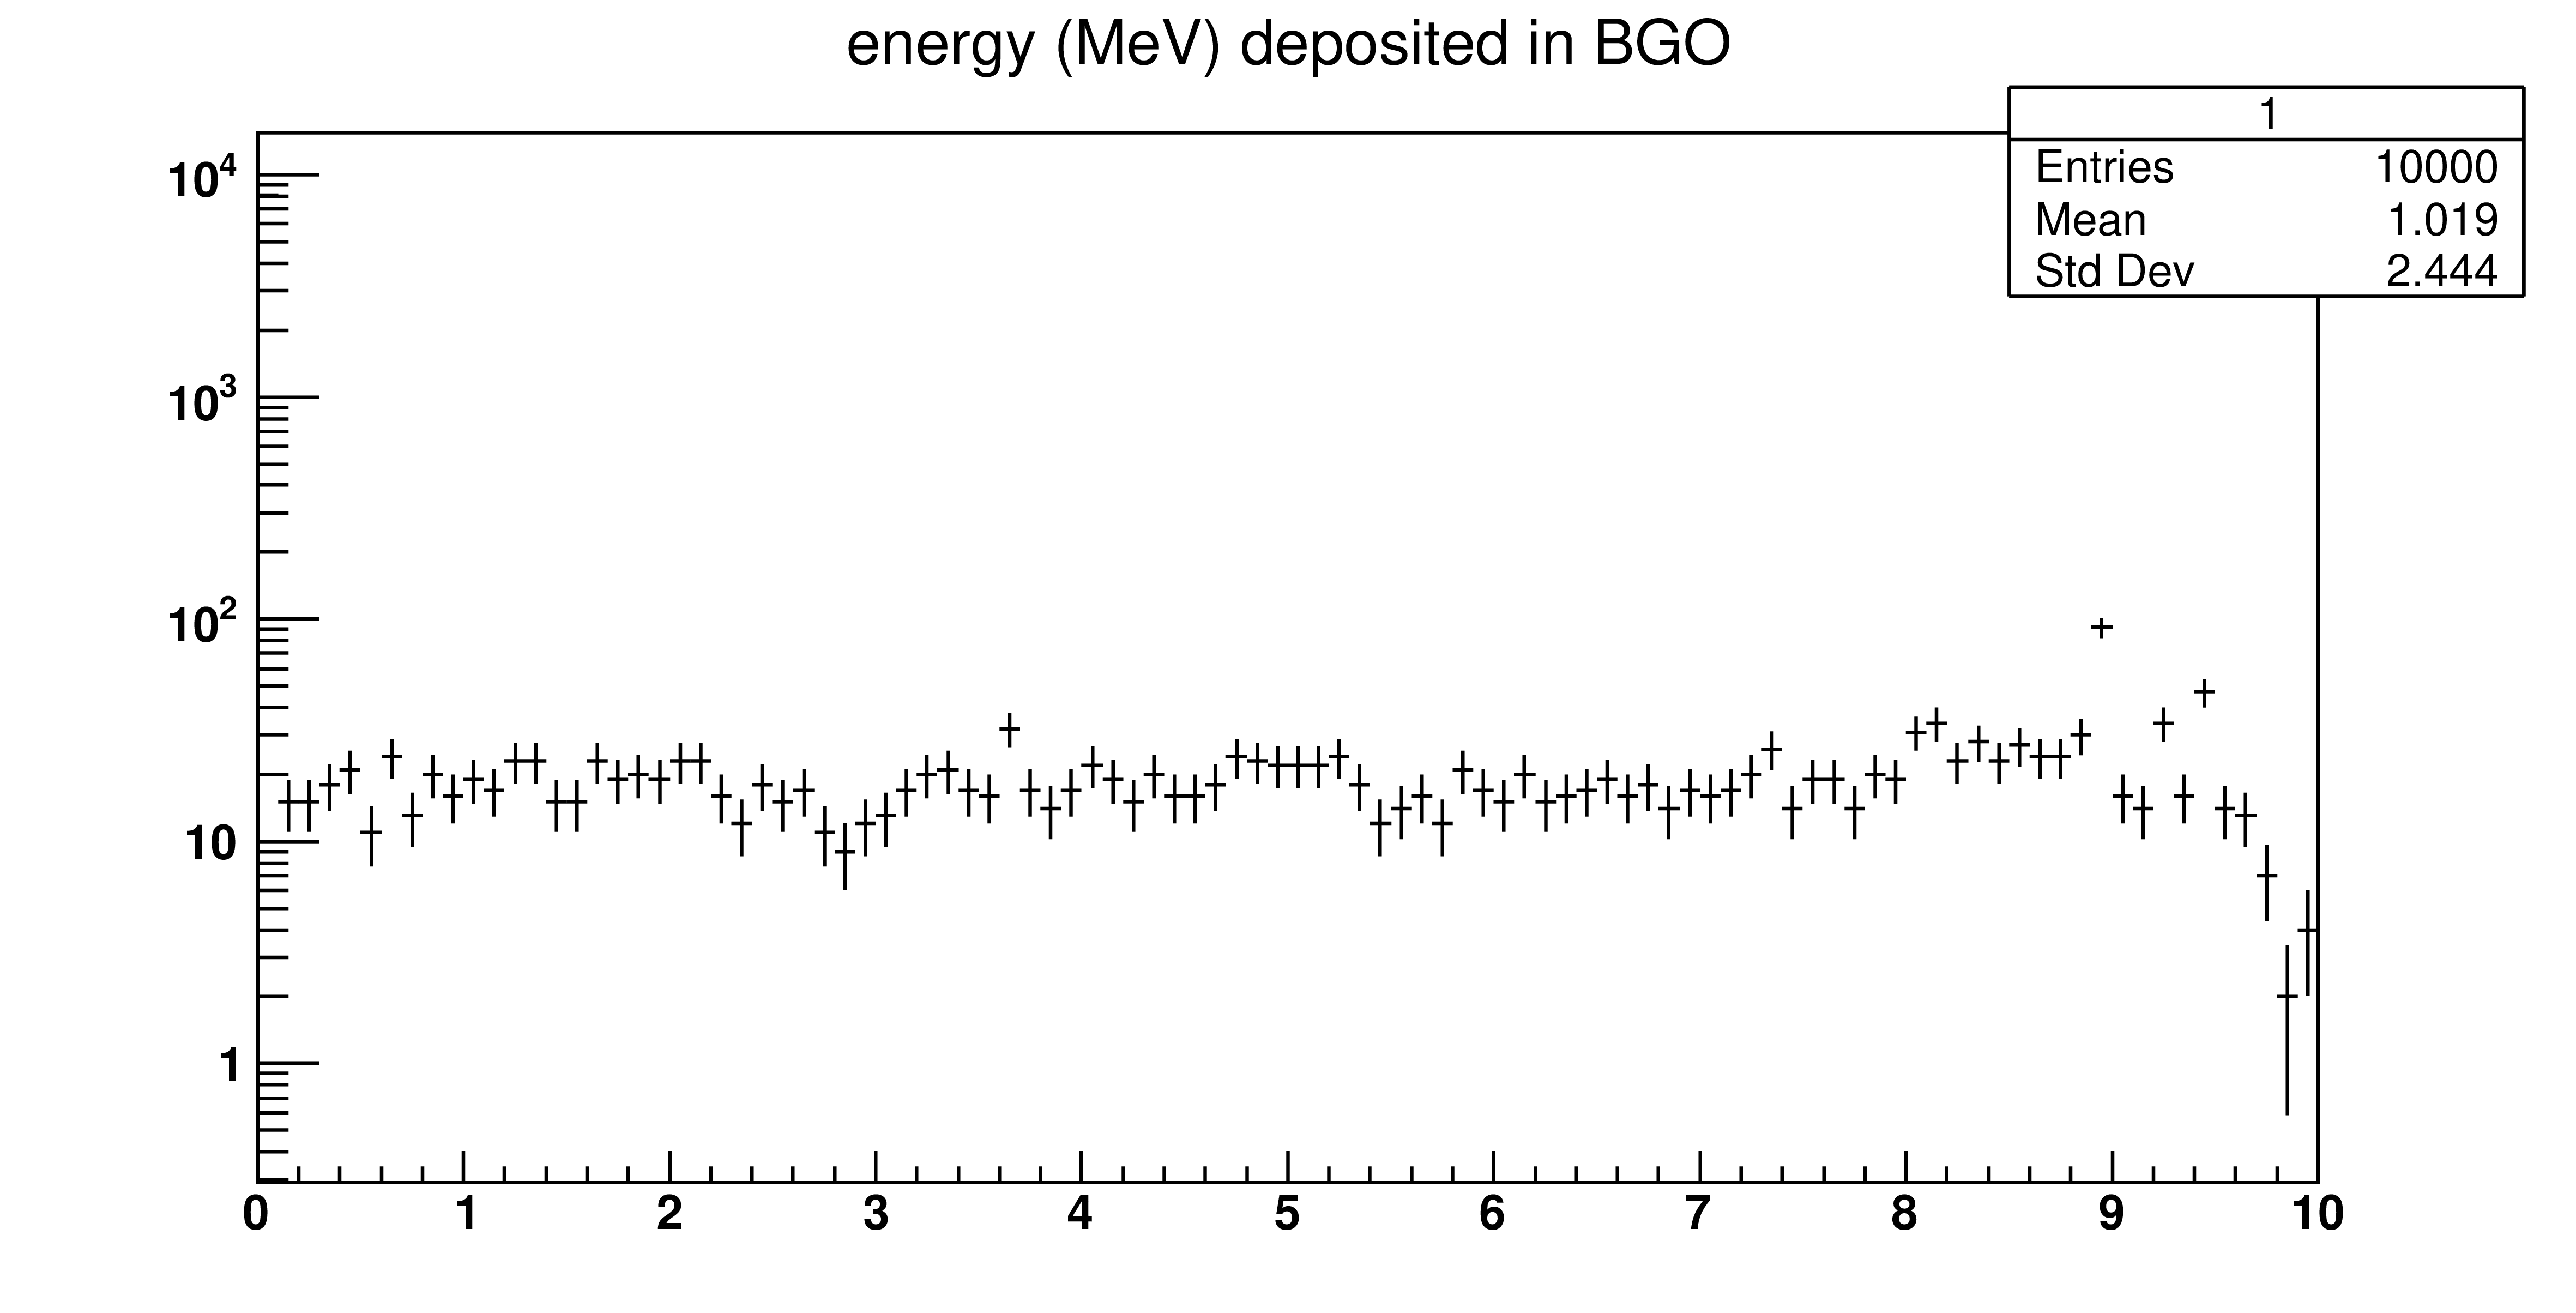
\includegraphics[width=\linewidth]{images/task1/BGO_10MeV.png}
  \caption{Deposited energy in BGO at 10 MeV incident energy}
\end{subfigure}%
\begin{subfigure}{.5\textwidth}
  \centering
  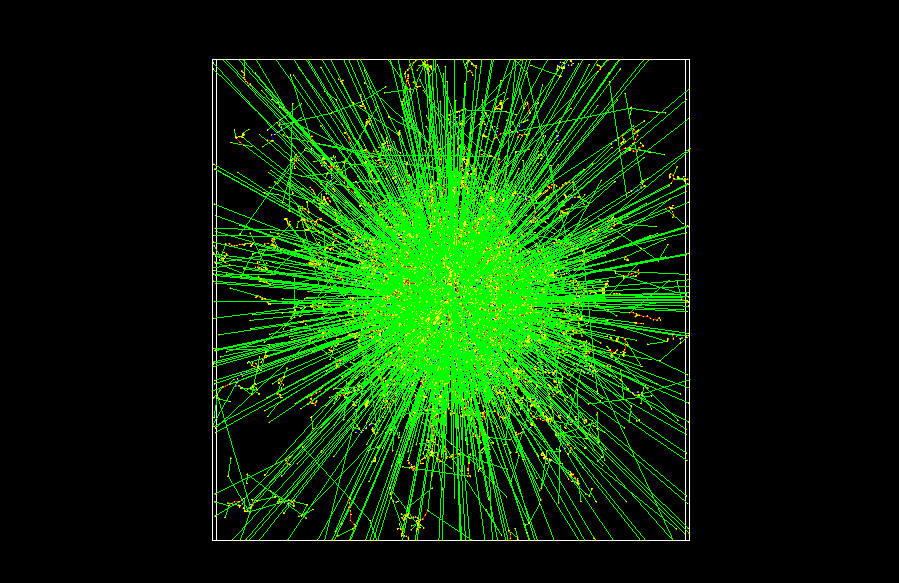
\includegraphics[width=\linewidth]{images/task1/BGO_10MeV_10000.png}
  \caption{Visualisation of the particle tracks}
\end{subfigure}
\caption{Results – BGO – 10 MeV}
\end{figure}


\subsubsection{LYSO}

\begin{figure}[H] % "[t!]" placement specifier just for this example
\begin{subfigure}{0.5\textwidth}
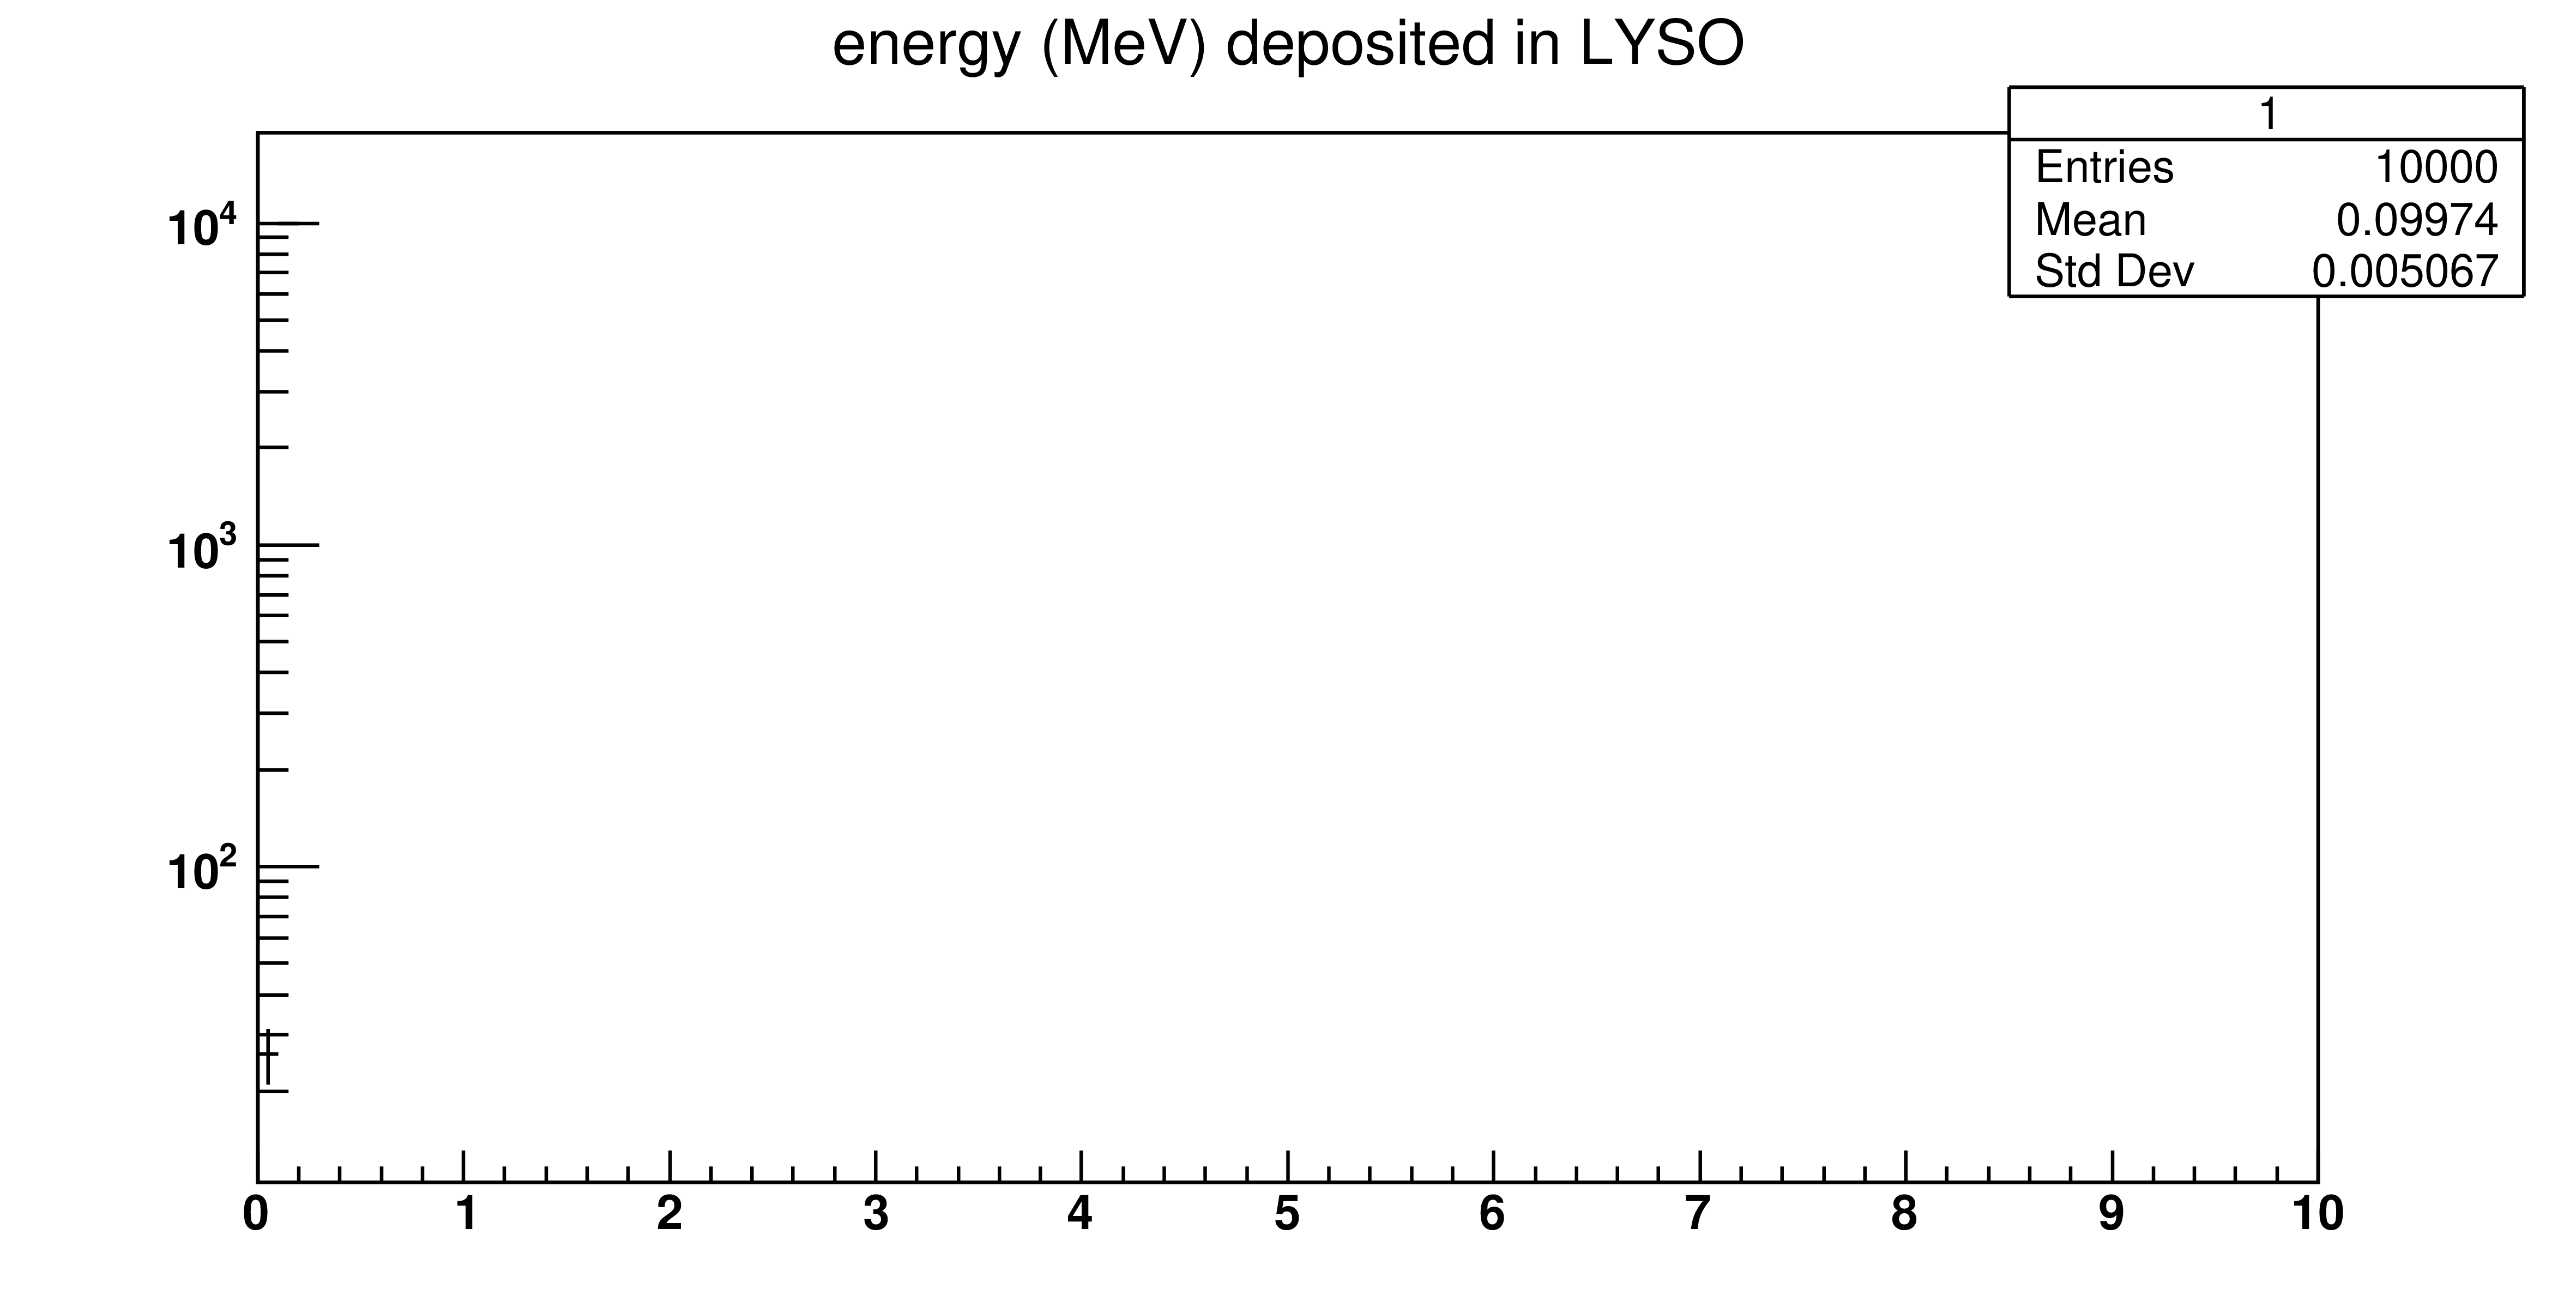
\includegraphics[width=\linewidth]{images/task1/LYSO_01MeV.png}
\caption{LYSO - 0.1 MeV} 
\end{subfigure}\hspace*{\fill}
\begin{subfigure}{0.5\textwidth}
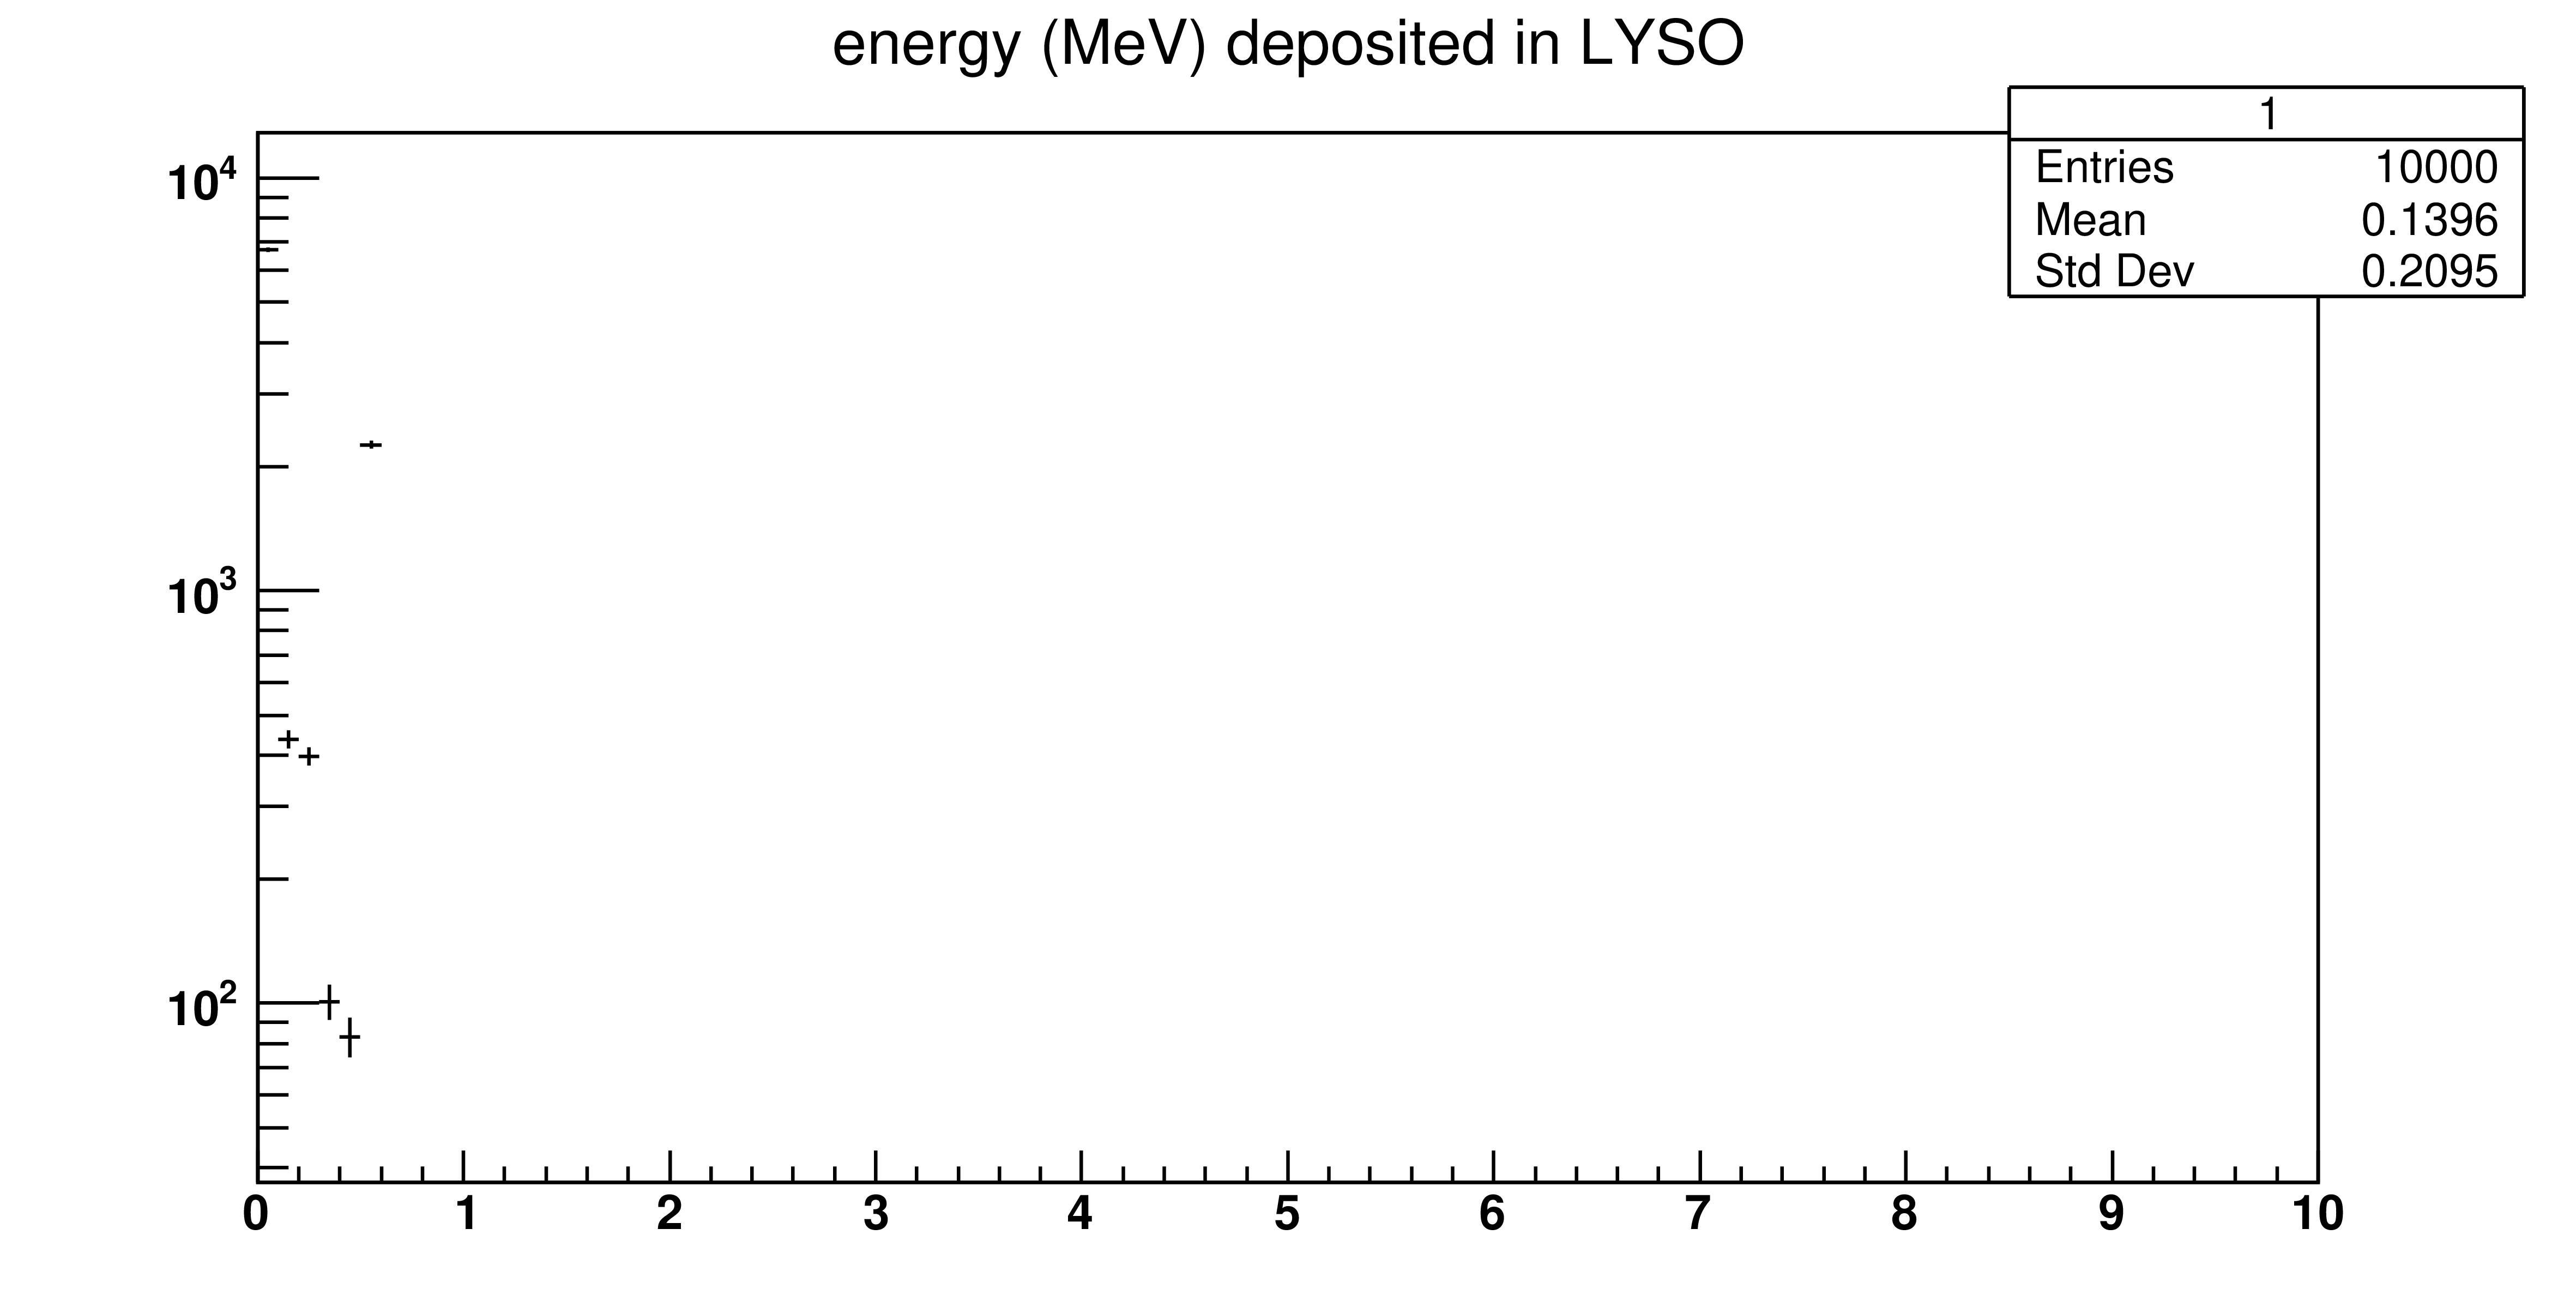
\includegraphics[width=\linewidth]{images/task1/LYSO_05MeV.png}
\caption{LYSO - 0.5 MeV} 
\end{subfigure}

\medskip
\begin{subfigure}{0.48\textwidth}
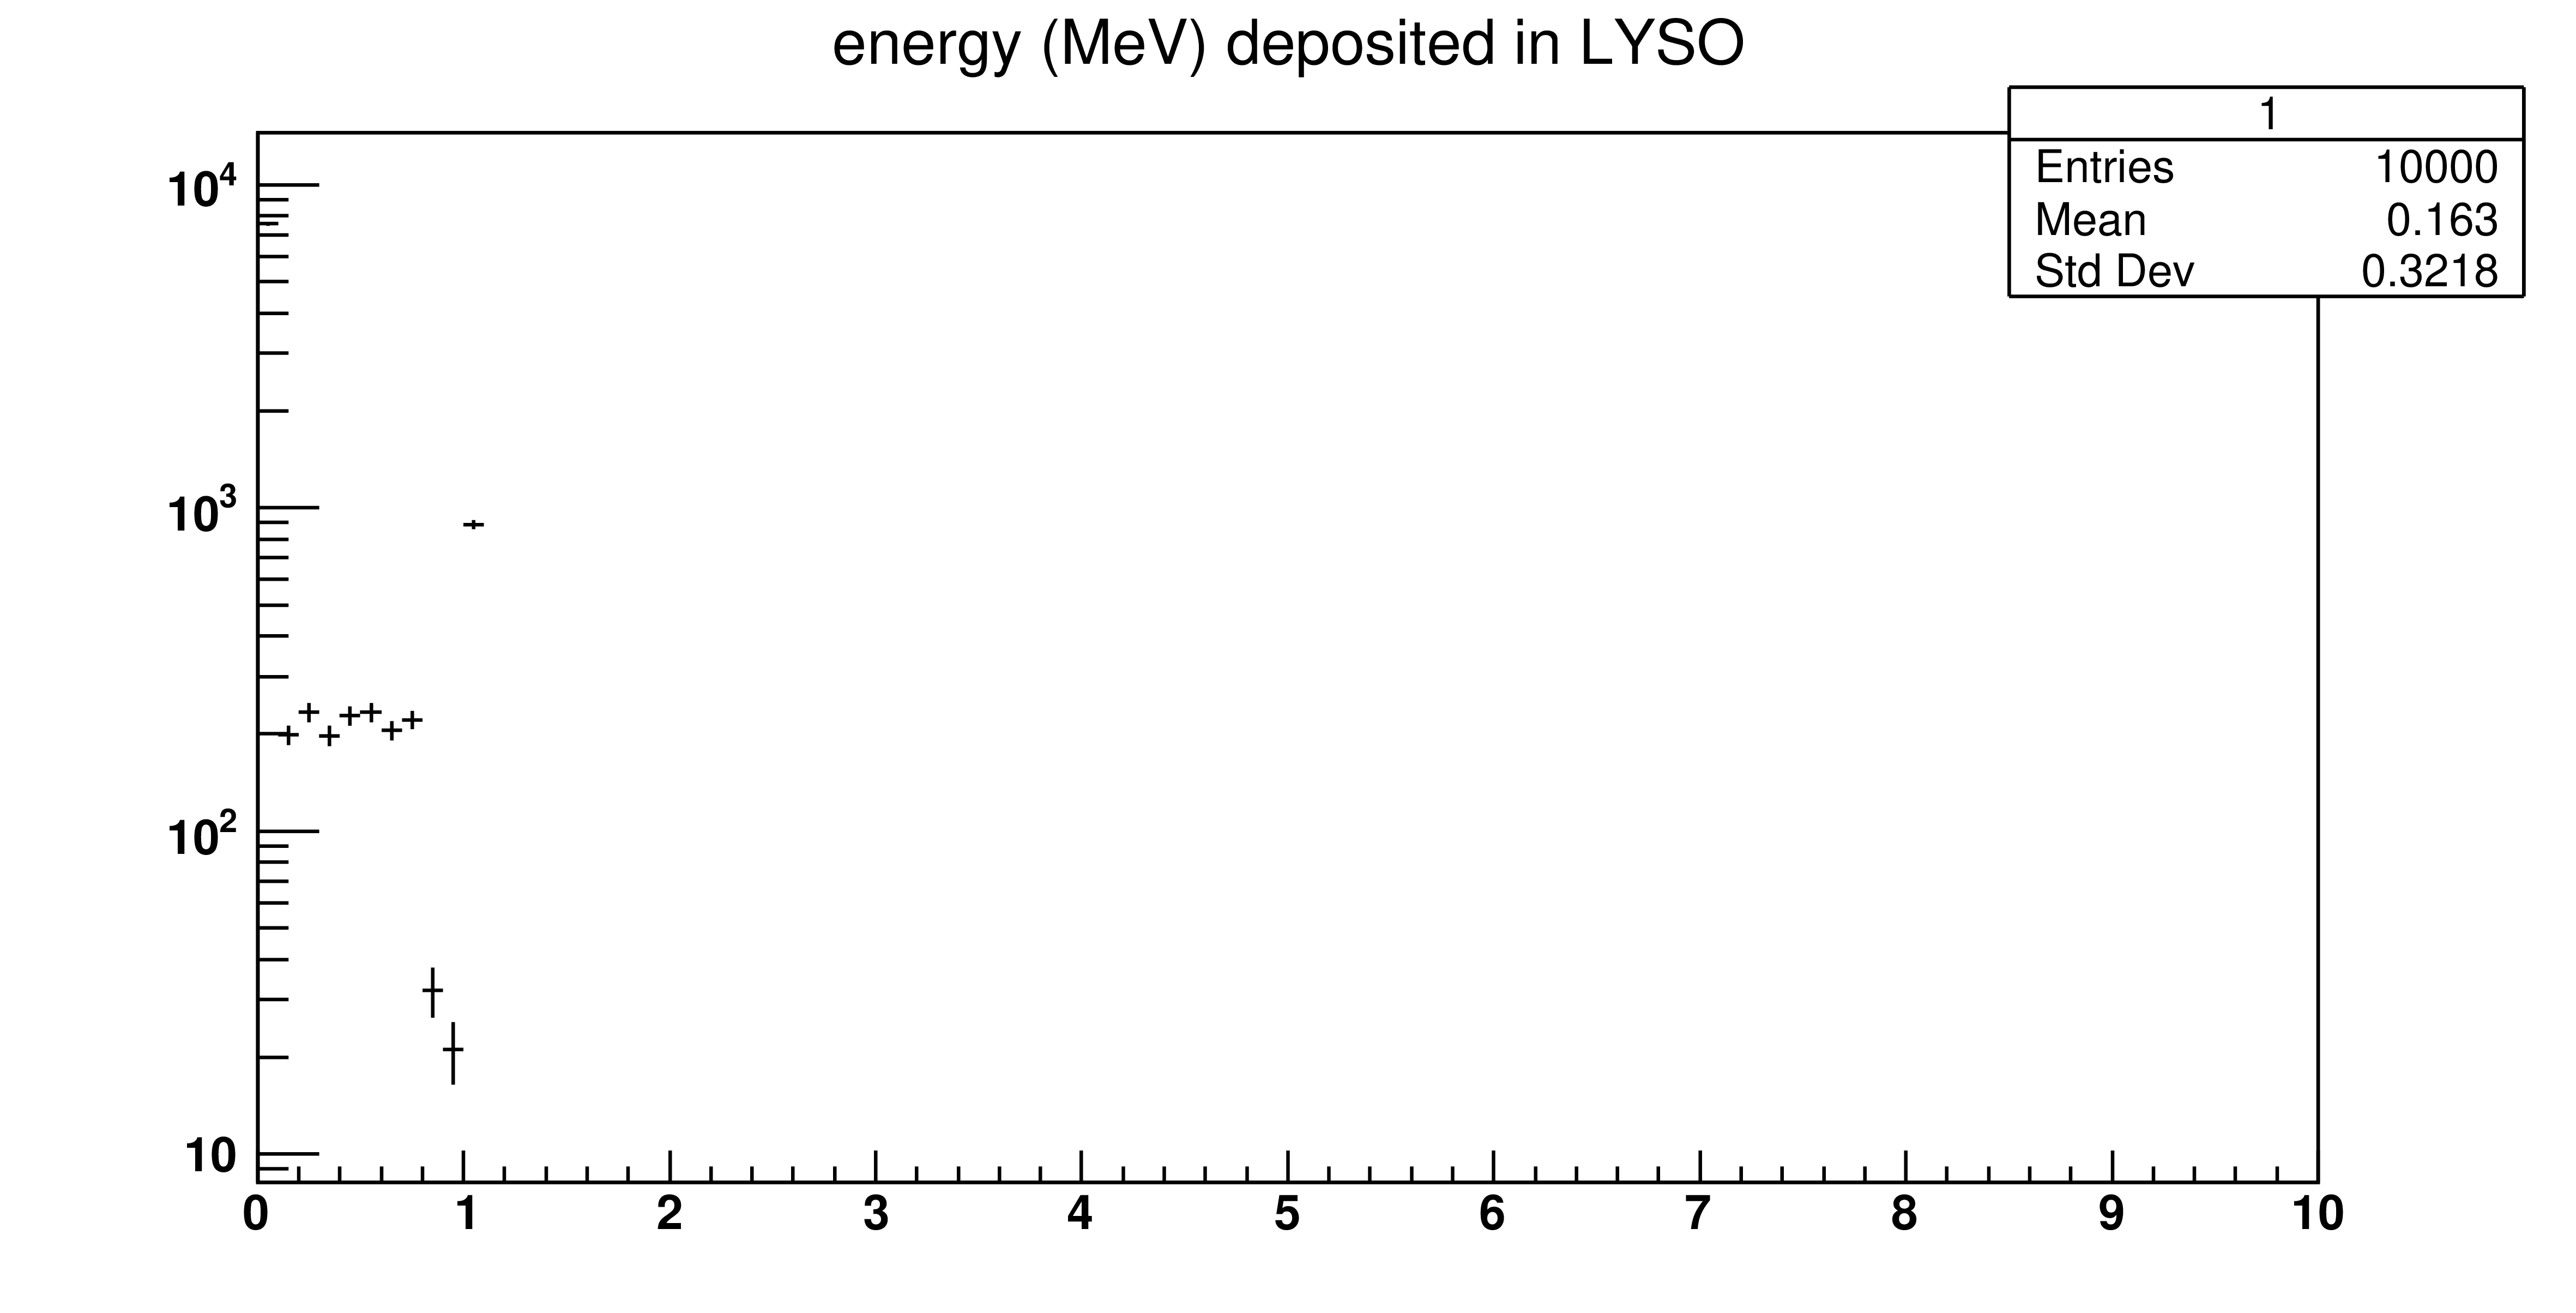
\includegraphics[width=\linewidth]{images/task1/LYSO_1MeV.png}
\caption{LYSO - 1 MeV}
\end{subfigure}\hspace*{\fill}
\begin{subfigure}{0.48\textwidth}
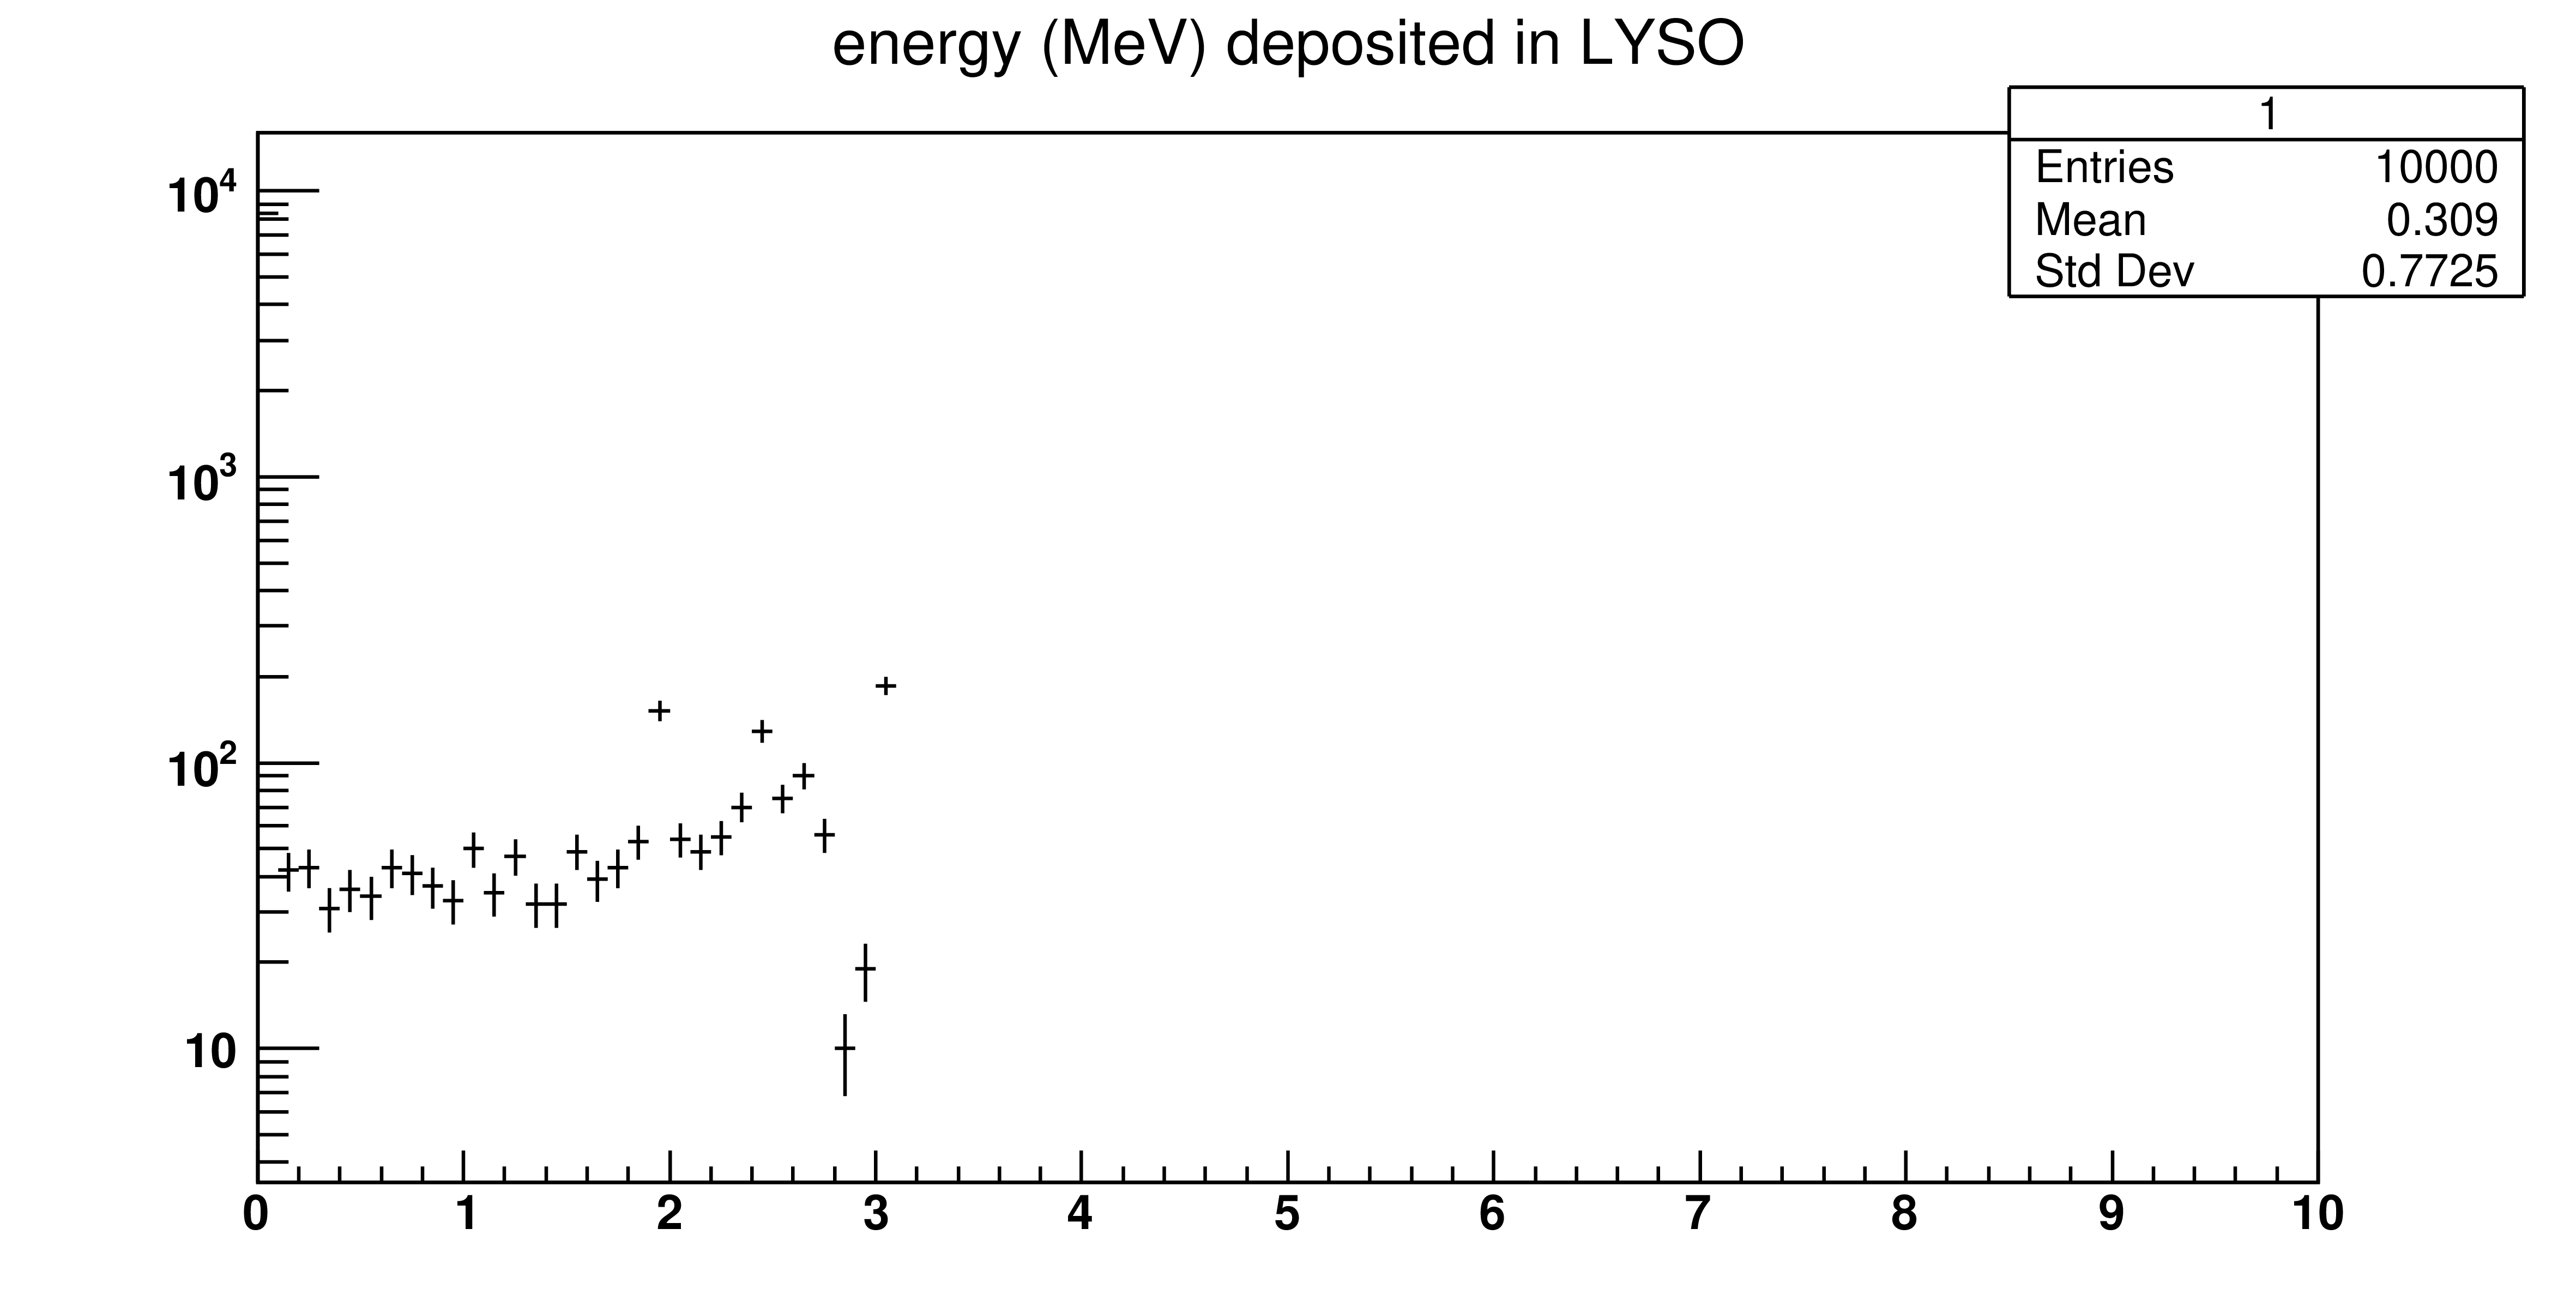
\includegraphics[width=\linewidth]{images/task1/LYSO_3MeV.png}
\caption{LYSO - 3 MeV} 
\end{subfigure}

\medskip
\begin{subfigure}{0.48\textwidth}
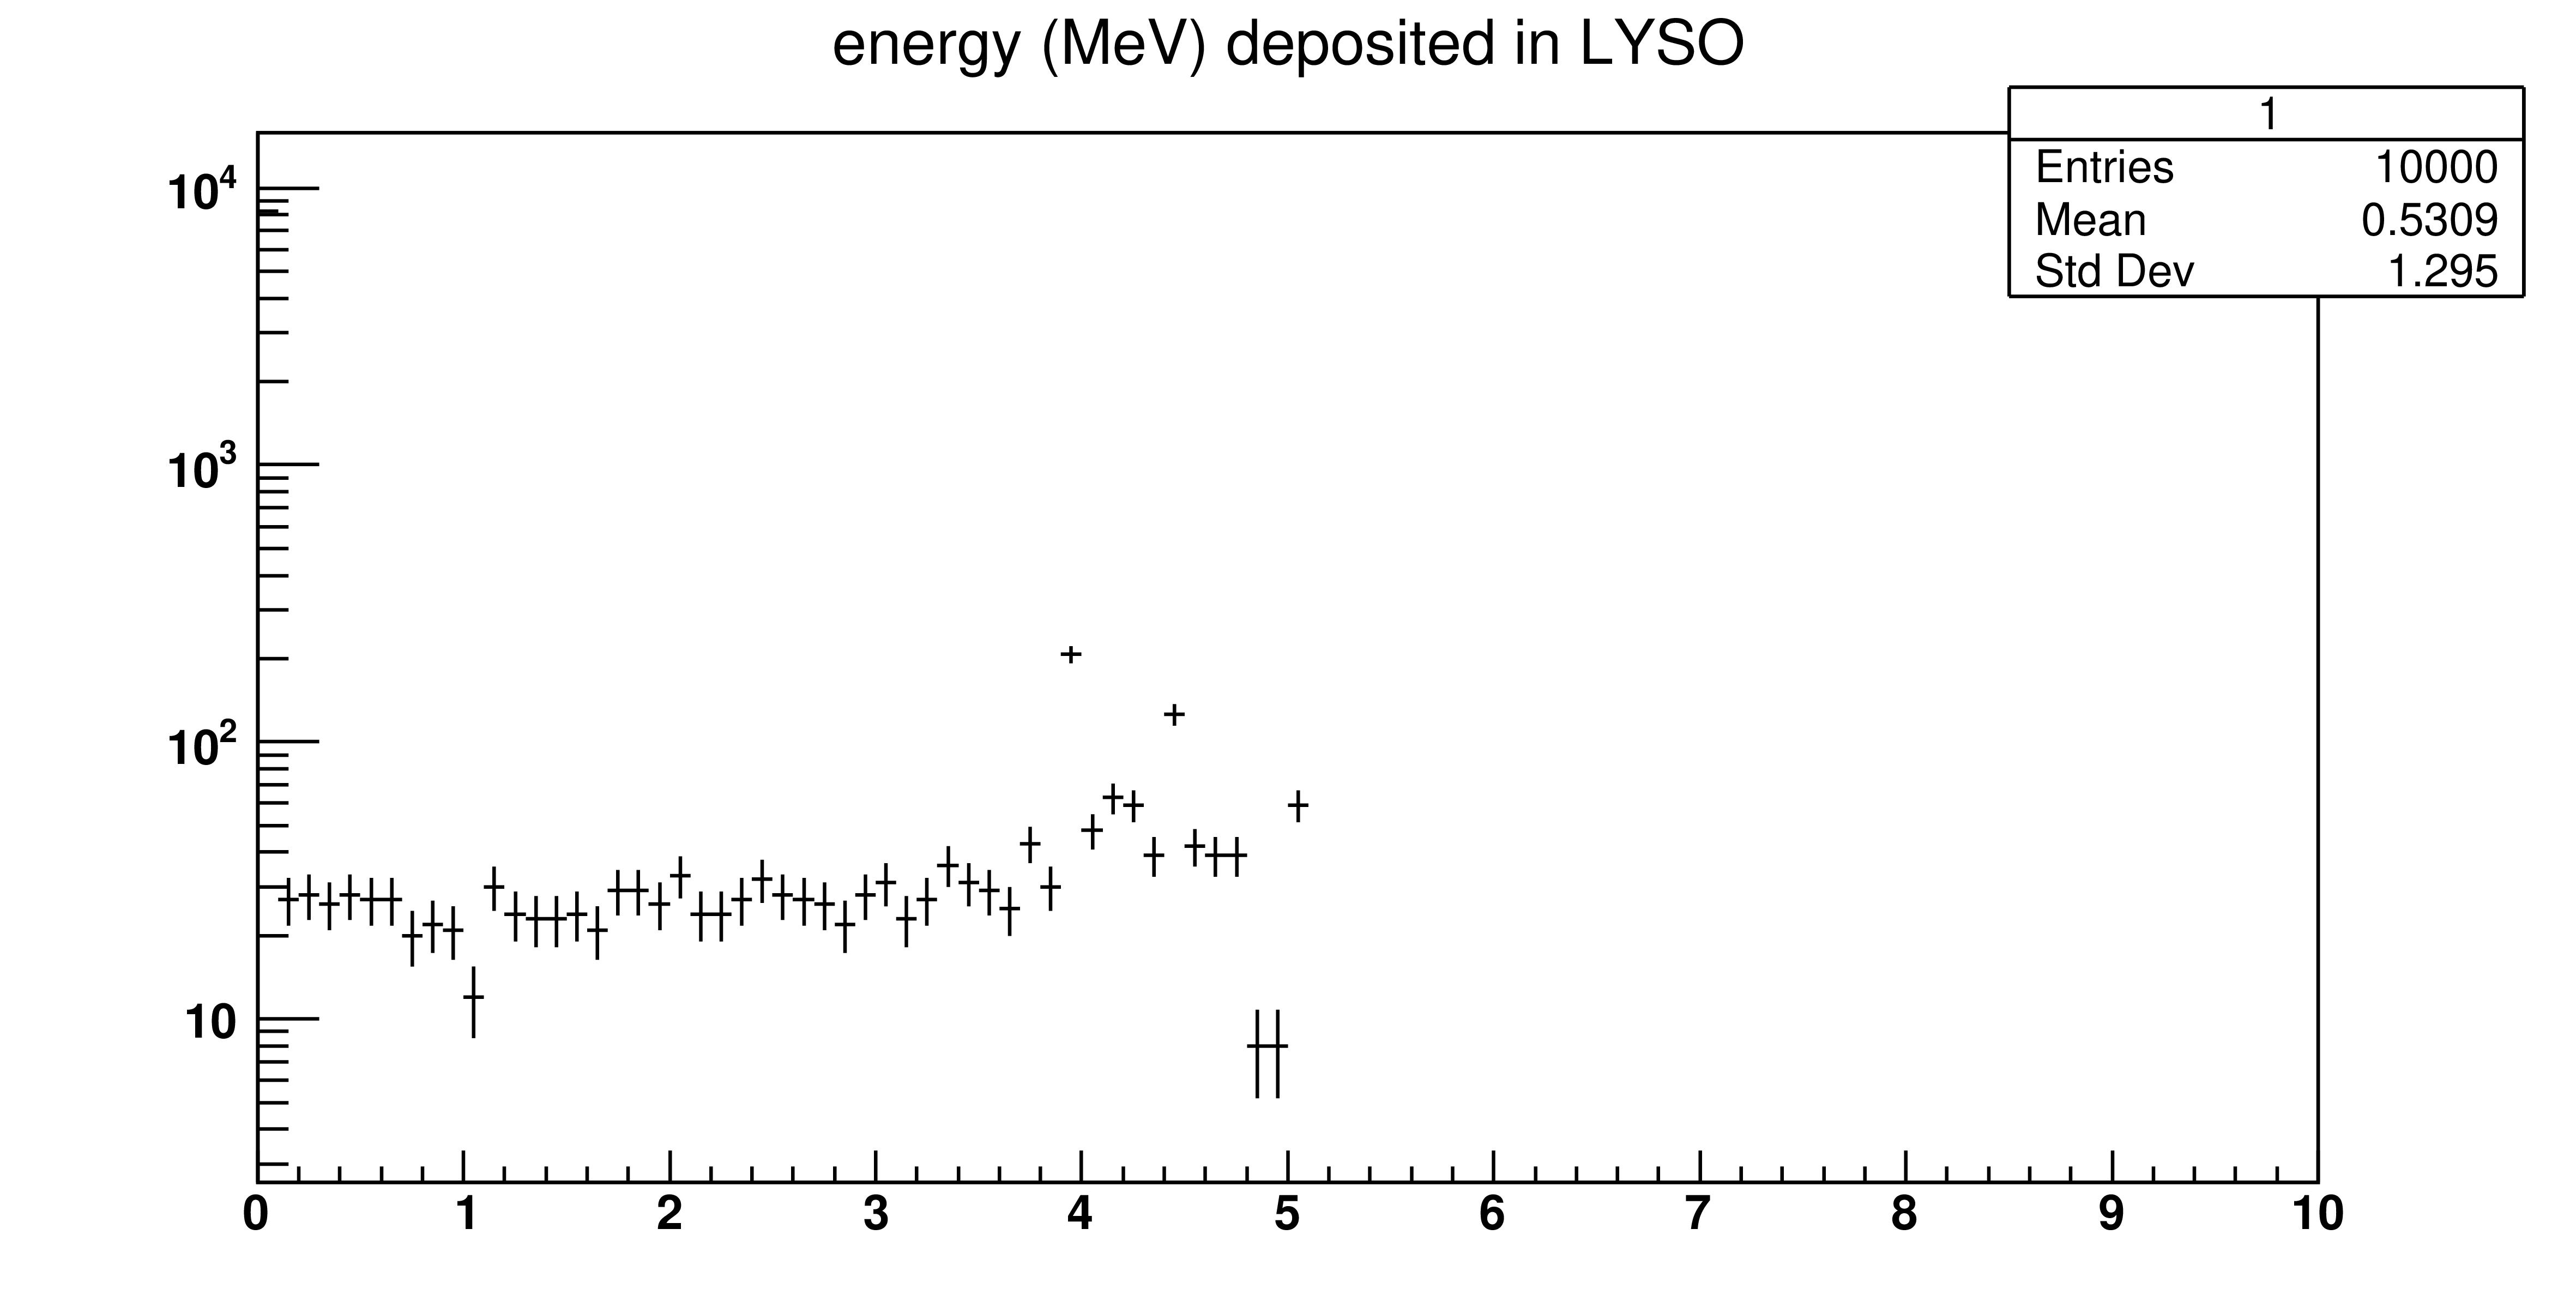
\includegraphics[width=\linewidth]{images/task1/LYSO_5MeV.png}
\caption{LYSO - 5 MeV}
\end{subfigure}\hspace*{\fill}
\begin{subfigure}{0.48\textwidth}
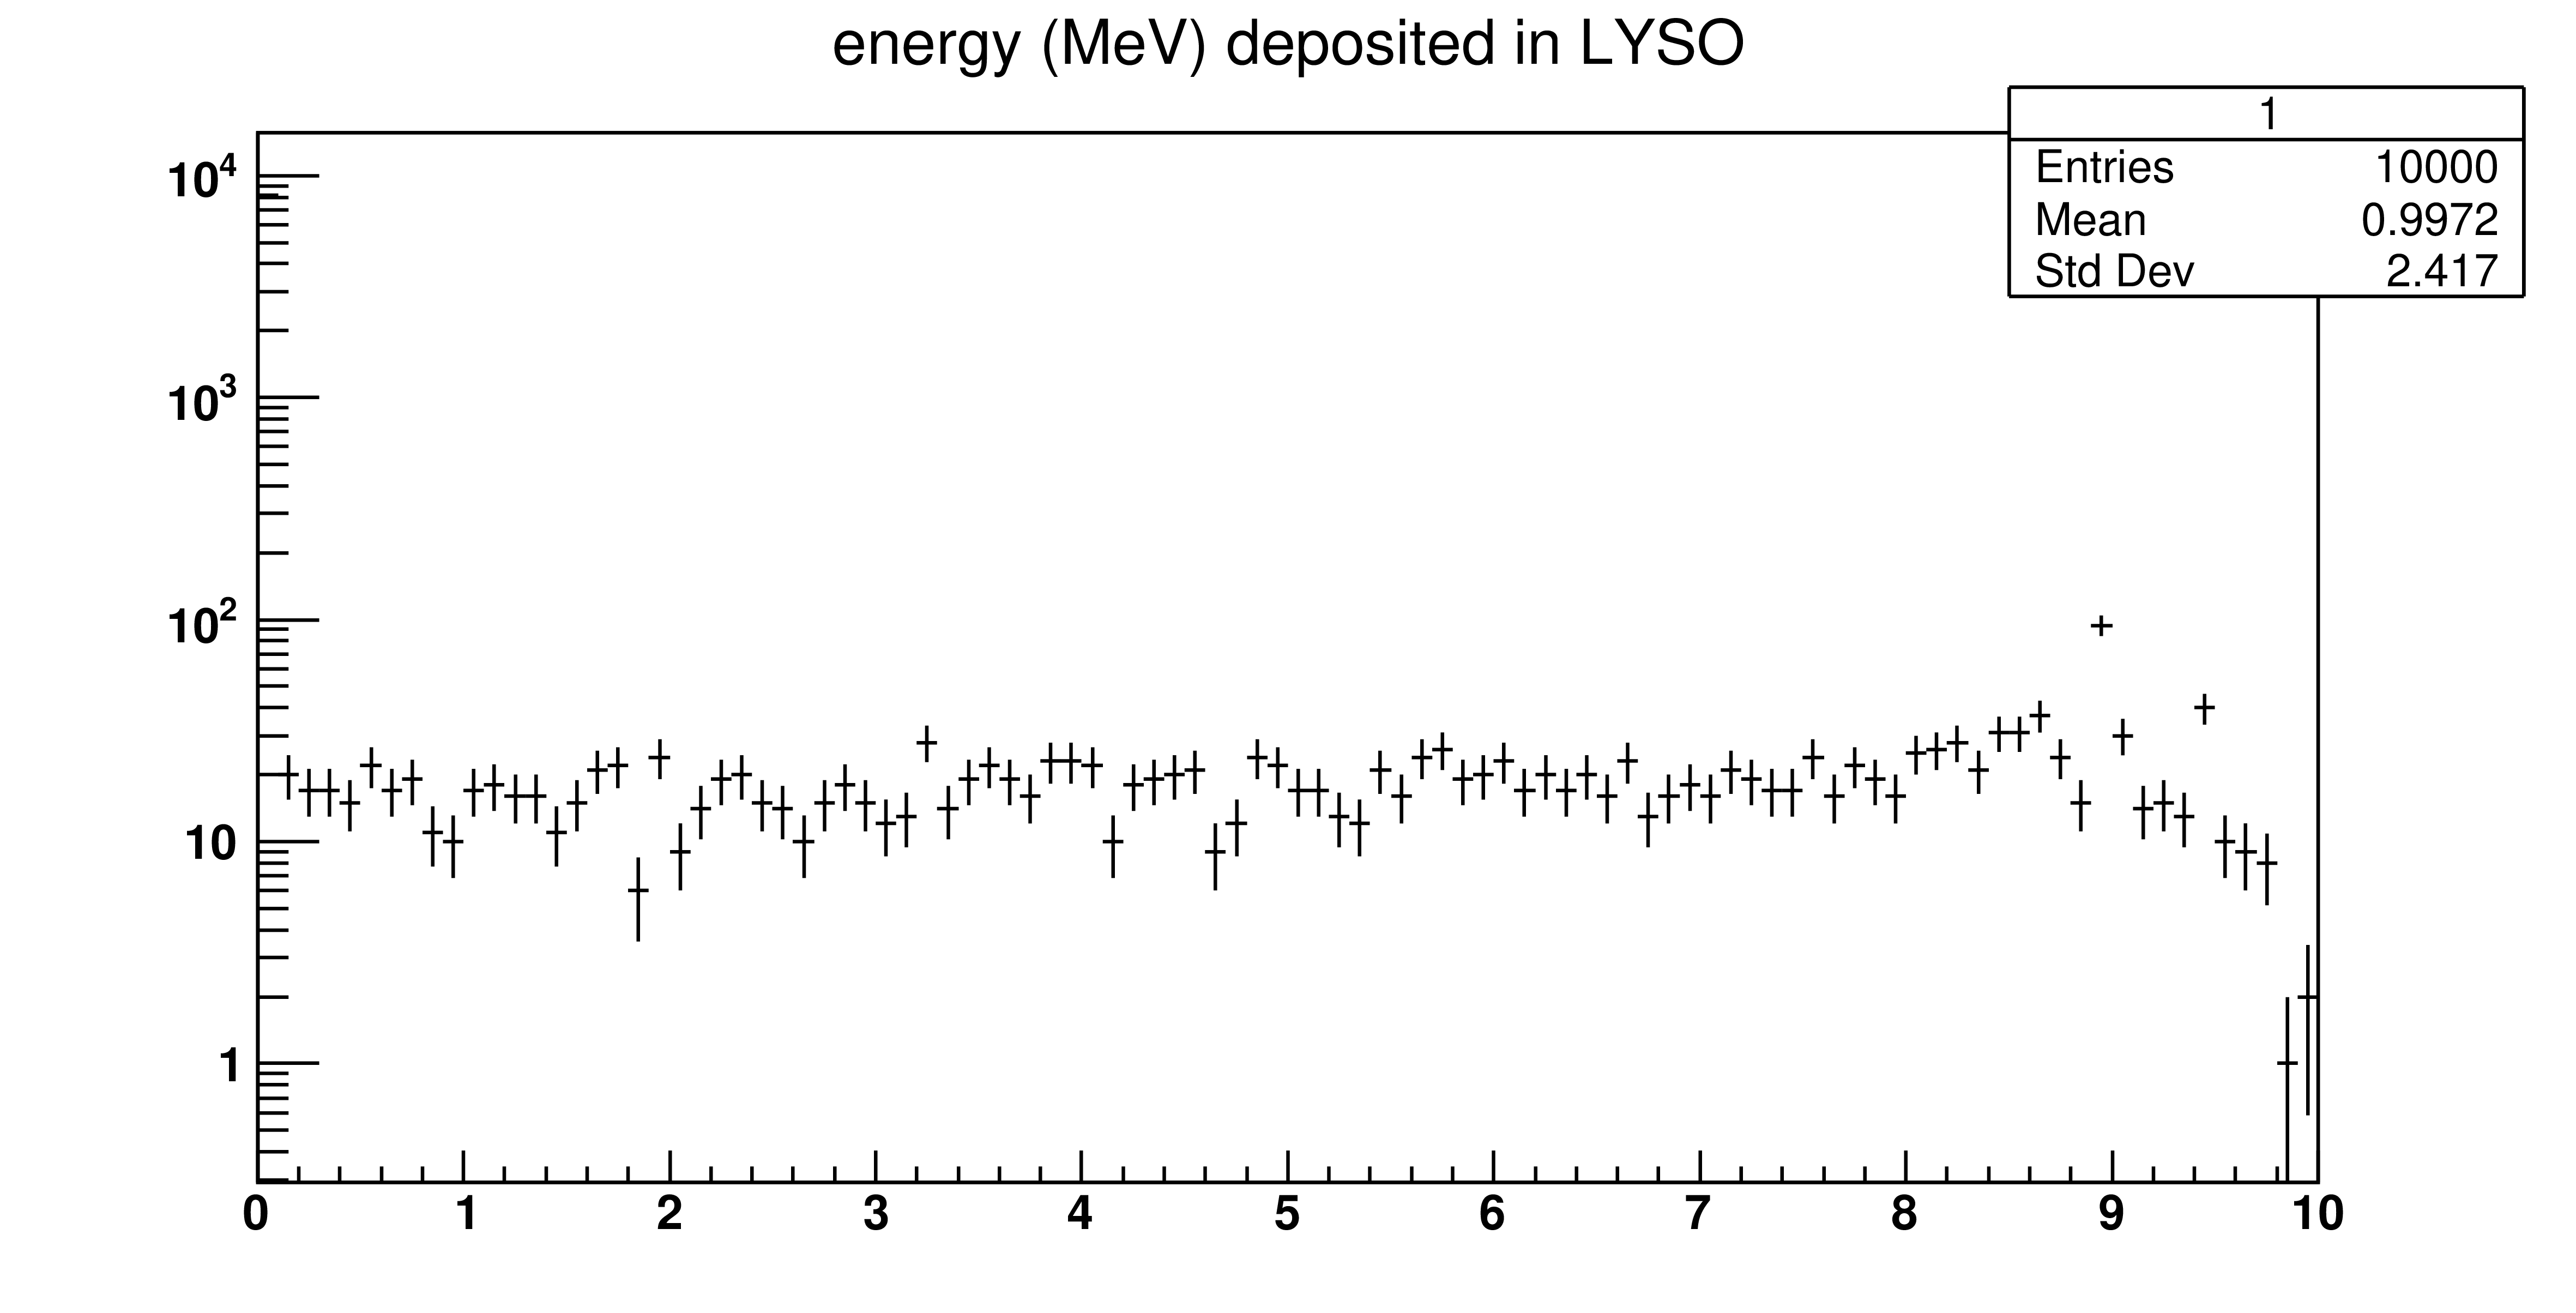
\includegraphics[width=\linewidth]{images/task1/LYSO_10MeV.png}
\caption{LYSO - 10 MeV} 
\end{subfigure}

\end{figure}

\subsection{Task 2. Calculate the energy deposition (first)}

Cum am calculat energia depusă din fiecare simulare: (\href{https://github.com/rmiron30/tasks_geant4/blob/main/scintillator_task/optical_yield_task/histo_code.py}{link})


% \begin{lstlisting}[language=Python]

% from ROOT import TFile, gPad


% file = TFile("testem4.root")

% hist = file.Get("Hist")

% hist.Draw("hist")
% gPad.WaitPrimitive("ggg")

% x_values = []
% y_values = []
% E = 0
% total_energy=0.0
% print(hist.GetNbinsX())


% for i in range(1, hist.GetNbinsX() + 1):

%     #energy_bin = hist.GetBinCenter(i)
%     #counts = hist.GetBinContent(i)
%     #total_energy += energy_bin * counts
%     x_values.append(hist.GetBinCenter(i))
%     y_values.append(hist.GetBinContent(i))
    
% for i in range(len(x_values)):
% 	E+=x_values[i]*y_values[i]

% #total_energy=hist.Integral()

% '''
% print("X values:")
% print(x_values)

% print("Y values:")
% print(y_values)
% '''
% print(E, "MeV")
% print(hist.GetEntries())

% #hist.Draw("hist")

% #gPad.WaitPrimitive("ggg")
    
% \end{lstlisting}

% Programul care reprezintă graficele din această secțiune:

% \begin{lstlisting}[language=Python]

% import pandas as pd
% import matplotlib.pyplot as plt


% data = pd.read_csv('data_CsI.txt', delimiter='\t')


% energies = data['E (MeV)'].unique()


% plt.figure(figsize=(10, 6))
% for energy in energies:
%     filtered_data = data[data['E (MeV)'] == energy]
%     width_cm = filtered_data['width (cm)']
%     e_dep_mev = filtered_data['E_dep/part (MeV/part)']
%     plt.plot(width_cm, e_dep_mev, marker='o', linestyle='--', label=f'E = {energy} MeV')

% plt.title('Deposited energy as function of layer thickness in CsI(Tl)')
% plt.xlabel('thickness (cm)')
% plt.ylabel('Deposited energy per photon (MeV/particle)')
% plt.legend()
% plt.grid(True)
% plt.show()

% \end{lstlisting}

\begin{figure}[H]

  \centering
  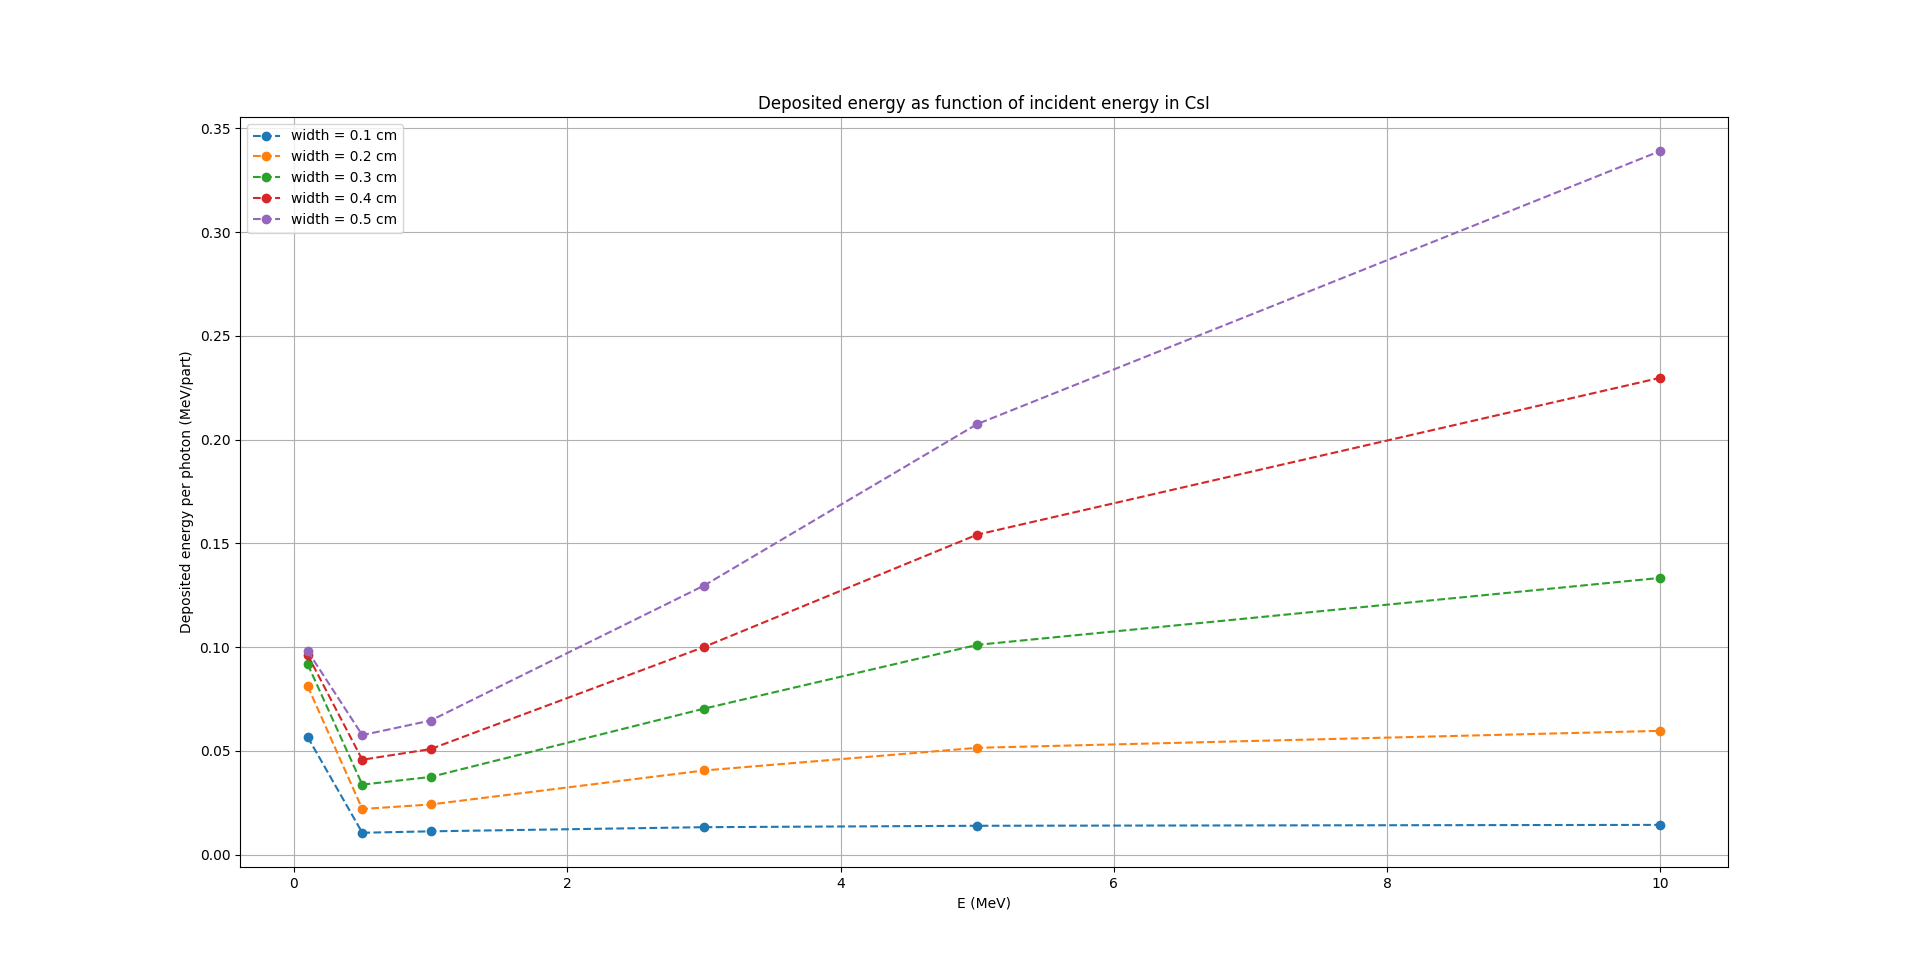
\includegraphics[width=\linewidth]{images/task2/dep_energy_en_CsI_particle.png}
  %\caption{Deposited energy in BGO at 5 MeV incident energy}

\end{figure}

\begin{figure}[H]
  \centering
  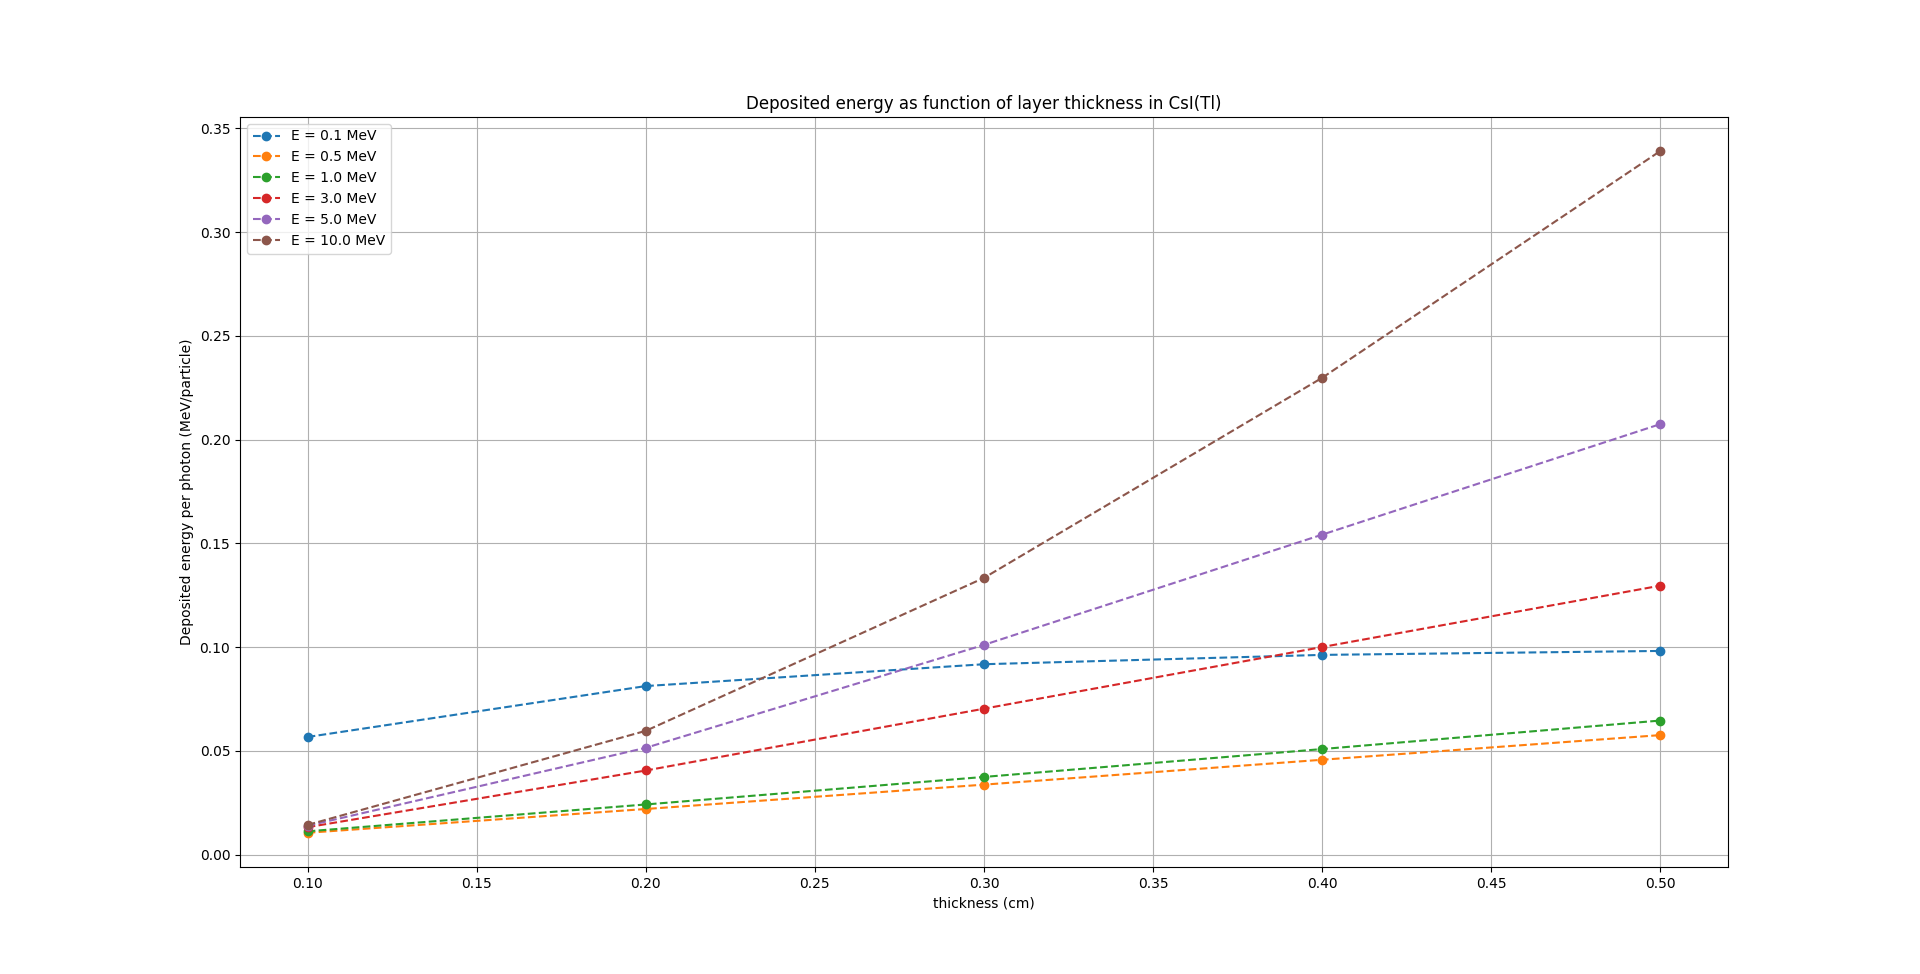
\includegraphics[width=\linewidth]{images/task2/dep_energy_thickness_CsI_particle.png}
  %\caption{Visualisation of the deposited energy}
\end{figure}

\begin{figure}[H]
  \centering
  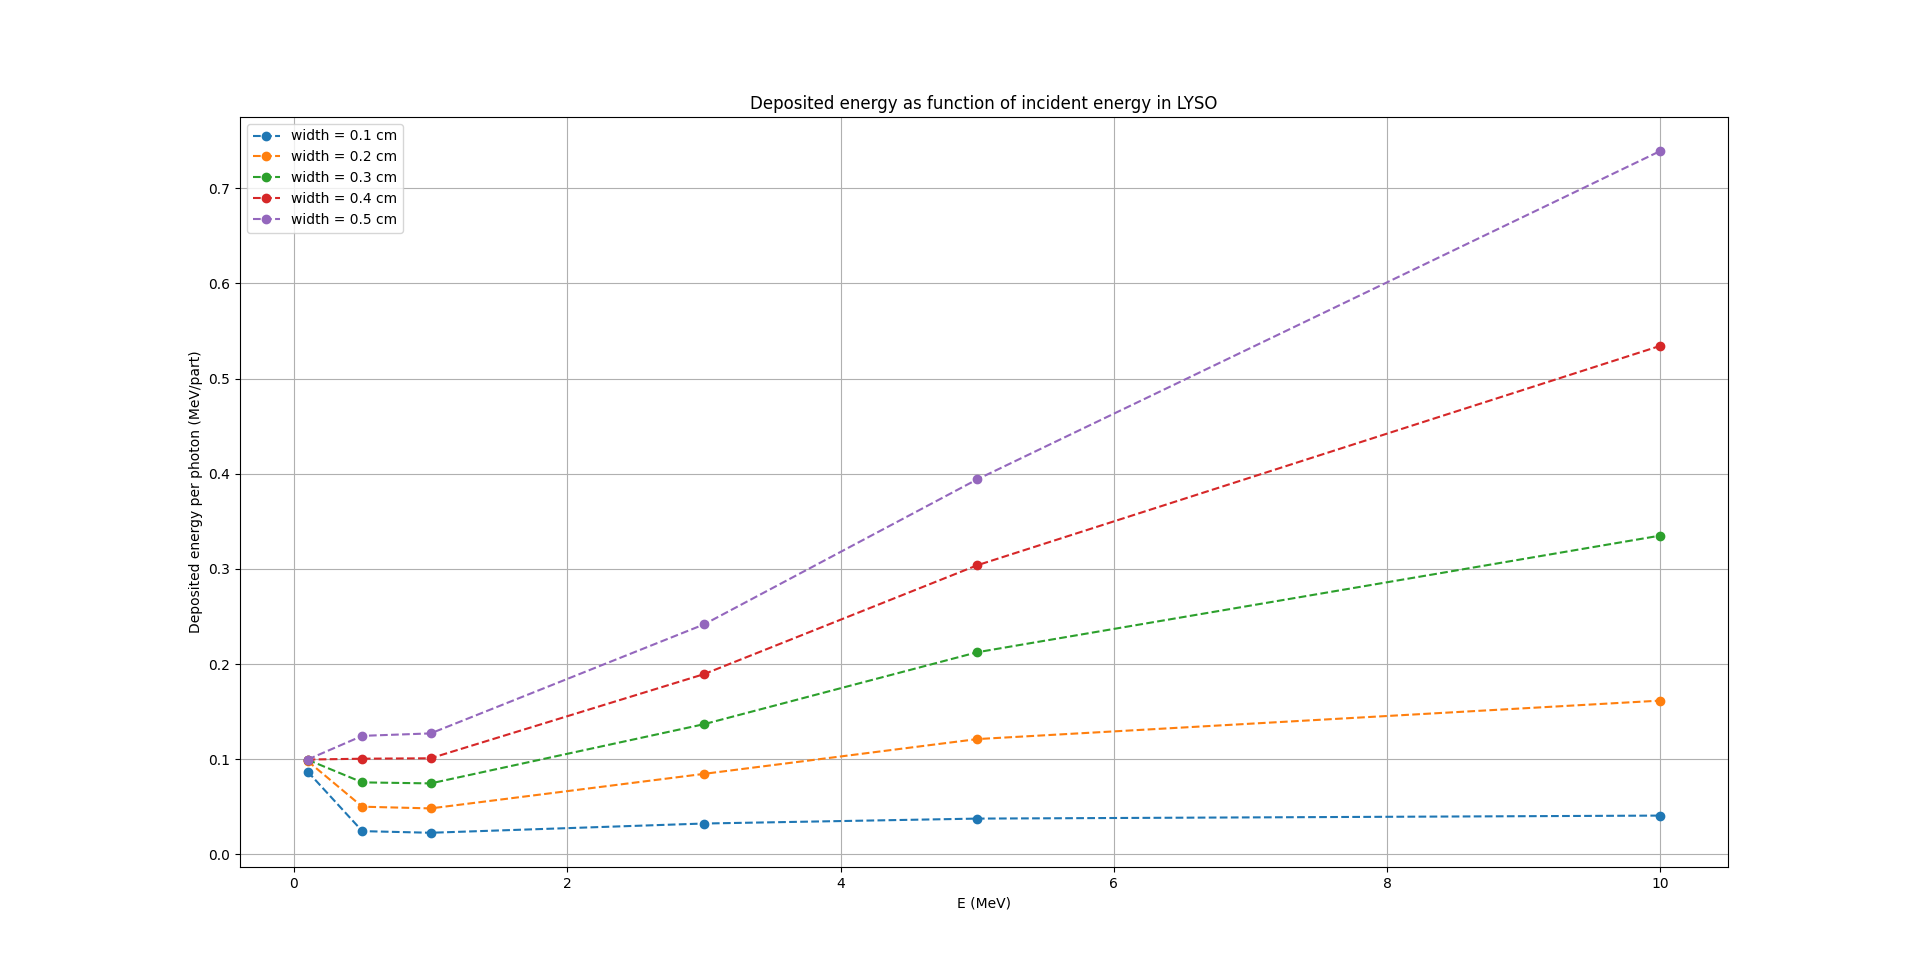
\includegraphics[width=\linewidth]{images/task2/dep_energy_en_LYSO_particle.png}
  %\caption{Deposited energy in BGO at 10 MeV incident energy}
\end{figure}

\begin{figure}[H]
  \centering
  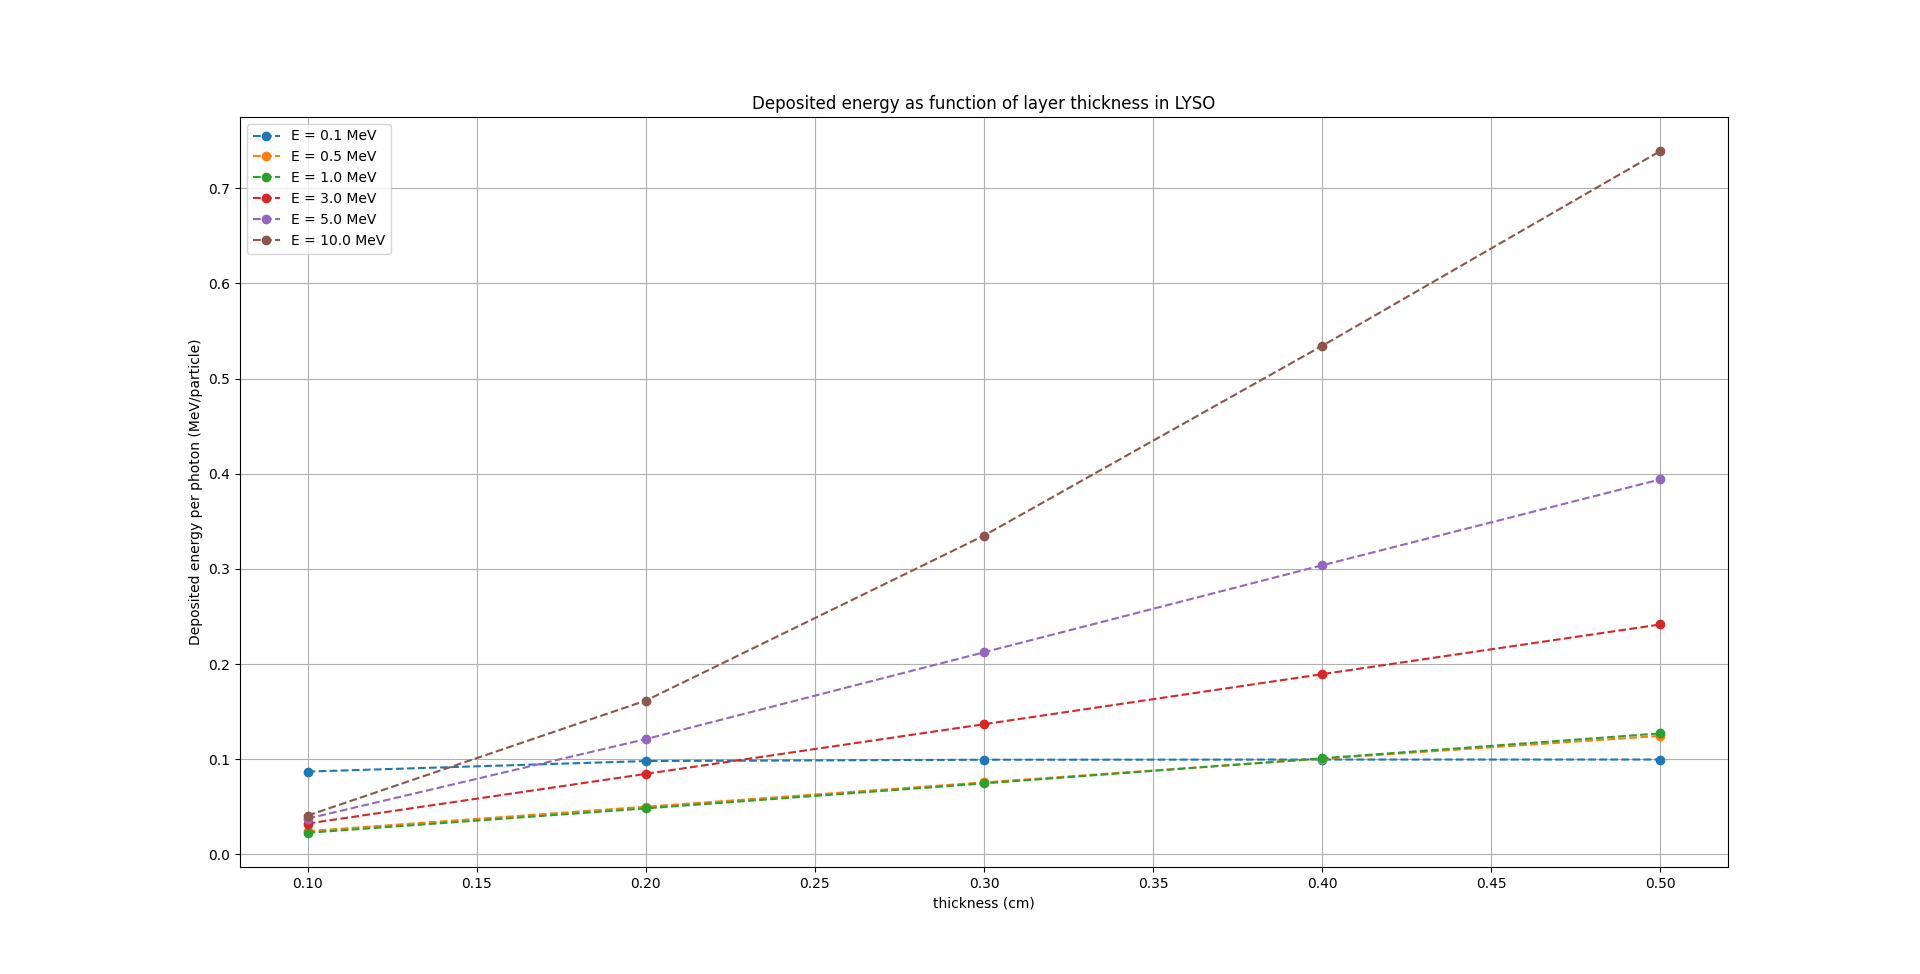
\includegraphics[width=\linewidth]{images/task2/dep_energy_thickness_LYSO_particle.png}
  %\caption{Visualisation of the deposited energy}
\end{figure}

\subsection{Task 3. Calculate the deposited energy and the number of scintillations produced in each material}

The code that was used to obtain the results and plots in this section: \href{https://github.com/rmiron30/tasks_geant4/blob/main/scintillator_task/optical_yield_task/myDesing.py}{link}

The number of interacting photons can be obtained with the following formula. Further, we can use this to verify that the number of entries provided by GEANT4 is acceptable.

\begin{equation*}
    N_{interactions} = N_0 (1-\text{e}^{-\mu \cdot x})
\end{equation*}

The number of optical photons (scintillations) produced by the interaction with gamma photons is given by:

\begin{equation*}
    \text{optical yield per interacting particle} = \frac{\text{deposited energy}}{\text{entries}} \cdot \text{light yield}
\end{equation*}
\begin{equation*}
    \text{total optical yield} = \text{deposited energy} \cdot \text{light yield}
\end{equation*}

\begin{table}[H]
    \centering
    \begin{tabular}{|ccccc|}
    \hline
        material &   $\rho$ ($g/cm^3$)&yield (ph/keV)&E (MeV) & $\mu$ (cm$^{-1}$) \\ \hline
        \multirow{6}{*}{CsI(Tl)} &   \multirow{6}{*}{4.51}&\multirow{6}{*}{54}&0.1 & 9.17785 \\ 
         &   &&0.5 & 0.4423859 \\ 
         &   &&1 & 0.2637448 \\ 
         &   &&3 & 0.1678171 \\ 
         &   &&5 & 0.1633522 \\ 
         &   &&10 & 0.181753 \\ \hline
       \multirow{6}{*}{BGO} &   \multirow{6}{*}{7.1}&\multirow{6}{*}{8}&0.1 & 28.1941 \\ 
         &   &&0.5 & 0.98619 \\ 
         &   &&1 & 0.484504 \\ 
         &   &&3 & 0.286982 \\ 
         &   &&5 & 0.275267 \\ 
         &   &&10 & 0.301466 \\ \hline
        \multirow{6}{*}{LYSO} &   \multirow{6}{*}{7.4}&\multirow{6}{*}{40}&0.1 & 18.5 \\ 
         &   &&0.5 & 0.81918 \\ 
         &   &&1 & 0.463832 \\ 
         &   &&3 & 0.284604 \\ 
         &   &&5 & 0.26973 \\ 
         &   &&10 & 0.290006 \\ \hline
    \end{tabular}
    \caption{The density, yield and linear coefficients corresponding to each material and incident energy}
\end{table}

\begin{table}[H]
    \centering
    \begin{tabular}{|cccccccc|}
    \hline
        E (MeV) & thickness (mm) & $N_{G4}$ &  DE (MeV) &  DE($\frac{MeV}{part}$)  &  $N_{int}$  &  scintil.  &  total scintil. \\ \hline
         \multirow{3}{*}{0.1} & 0.5 & 741700 & 73185.138 & 0.099 & 755784.684 & 789.377 & 585481107.200 \\ 
         & 1 & 932826 & 92543.909 & 0.099 & 940358.879 & 793.665 & 740351270.560 \\ 
         & 2 & 995378 & 98979.817 & 0.099 & 996442.937 & 795.515 & 791838532.320 \\ \hline
        \multirow{3}{*}{0.5} & 0.5 & 48246 & 14631.719 & 0.303 & 48113.525 & 2426.186 & 117053755.280 \\ 
         & 1 & 91330 & 30342.555 & 0.332 & 93912.138 & 2657.839 & 242740441.680 \\ 
         & 2 & 171806 & 61453.63 & 0.358 & 179004.787 & 2861.536 & 491629037.680 \\ \hline
        \multirow{3}{*}{1} & 0.5 & 25319 & 10948.519 & 0.432 & 23934.125 & 3459.384 & 87588155.160 \\ 
         & 1 & 48203 & 24578.044 & 0.51 & 47295.408 & 4079.089 & 196624350.120 \\ 
         & 2 & 92002 & 52352.935 & 0.569 & 92353.96 & 4552.330 & 418823482.880 \\ \hline
        \multirow{3}{*}{3} & 0.5 & 15229 & 9840.736 & 0.646 & 14246.642 & 5169.472 & 78725888.120 \\ 
         & 1 & 29244 & 32508.677 & 1.112 & 28290.318 & 8893.086 & 260069418.400 \\ 
         & 2 & 56534 & 85053.088 & 1.504 & 55780.294 & 12035.672 & 680424703.200 \\ \hline
        \multirow{3}{*}{5} & 0.5 & 14589 & 9844.073 & 0.675 & 13669.068 & 5398.080 & 78752585.560 \\ 
         & 1 & 28260 & 38005.496 & 1.345 & 27151.293 & 10758.810 & 304043966.160 \\ 
         & 2 & 54868 & 123440.796 & 2.25 & 53565.393 & 17998.221 & 987526364.880 \\ \hline
        \multirow{3}{*}{10} & 0.5 & 15798 & 9917.915 & 0.628 & 14960.266 & 5022.365 & 79343322.960 \\ 
         & 1 & 30807 & 41340.75 & 1.342 & 29696.723 & 10735.417 & 330725996.920 \\ 
         & 2 & 59968 & 165331.96 & 2.757 & 58511.551 & 22056.024 & 1322655676.320 \\ \hline
    \end{tabular}
    \caption{Results obtained for $10^6$ incident photons in BGO material. Yield(BGO) = 8 photons/keV. The number of scintillations is calculated for the interacting particles. The column "scintil." represents scintillations per interacting particles, while the column "total scintil." refers to the entire beam. }
\end{table}

\begin{table}[H]
    \centering
    \begin{tabular}{|cccccccc|}
    \hline
       E (MeV) & thickness (mm) & $N_{G4}$ &  DE (MeV) &  DE($\frac{MeV}{part}$)  &  $N_{int}$  &  scintil.  &  total scintil. \\ \hline
        \multirow{3}{*}{0.1} & 0.5 & 352969 & 34075.292 & 0.097 & 368016.821 & 5213.109 & 1840065754.230 \\ 
         & 1 & 579259 & 56672.02 & 0.098 & 600597.261 & 5283.110 & 3060289054.350 \\ 
         & 2 & 821944 & 81223.12 & 0.099 & 840477.452 & 5336.189 & 4386048480.000 \\ \hline
        \multirow{3}{*}{0.5} & 0.5 & 23387 & 4950.17 & 0.212 & 21876.457 & 11429.820 & 267309192.150 \\ 
         & 1 & 43855 & 10482.999 & 0.239 & 43274.335 & 12908.036 & 566081931.690 \\ 
         & 2 & 83162 & 21941.315 & 0.264 & 84676.002 & 14247.264 & 1184830992.180 \\ \hline
        \multirow{3}{*}{1} & 0.5 & 14934 & 4732.622 & 0.317 & 13100.669 & 17112.733 & 255561562.080 \\ 
         & 1 & 27736 & 11179.311 & 0.403 & 26029.711 & 21765.316 & 603682799.940 \\ 
         & 2 & 52465 & 24125.558 & 0.46 & 51381.876 & 24831.414 & 1302780125.790 \\ \hline
        \multirow{3}{*}{3} & 0.5 & 9426 & 3599.809 & 0.382 & 8355.75 & 20622.715 & 194389707.600 \\ 
         & 1 & 17726 & 13174.569 & 0.743 & 16641.682 & 40134.645 & 711426713.580 \\ 
         & 2 & 34165 & 40490.142 & 1.185 & 33006.417 & 63997.297 & 2186467653.150 \\ \hline
        \multirow{3}{*}{5}& 0.5 & 8920 & 3406.614 & 0.382 & 8134.346 & 20622.999 & 183957148.980 \\ 
         & 1 & 17075 & 13853.369 & 0.811 & 16202.524 & 43811.532 & 748081904.130 \\ 
         & 2 & 33068 & 51422.718 & 1.555 & 32142.526 & 83973.231 & 2776826786.580 \\ \hline
        \multirow{3}{*}{10} & 0.5 & 9638 & 3566.448 & 0.37 & 9046.482 & 19982.175 & 192588200.640 \\ 
         & 1 & 18664 & 14282.154 & 0.765 & 18011.125 & 41322.134 & 771236318.160 \\ 
         & 2 & 36402 & 59606.751 & 1.637 & 35697.85 & 88422.739 & 3218764544.820 \\ \hline
    \end{tabular}
    \caption{Results obtained for $10^6$ incident photons in CsI(Tl) material. Yield(CsI(Tl)) = 54 photons/keV. The number of scintillations is calculated for the interacting particles. The column "scintil." represents scintillations per interacting particles, while the column "total scintil." refers to the entire beam. }
\end{table}

\newpage

\begin{table}[H]
    \centering
    \begin{tabular}{|cccccccc|}
    \hline
       E (MeV) & thickness (mm) & $N_{G4}$ &  DE (MeV) &  DE($\frac{MeV}{part}$)  &  $N_{int}$  &  scintil.  &  total scintil. \\ \hline
        \multirow{3}{*}{0.1} & 0.5 & 649348 & 64026.83 & 0.099 & 603468.581 & 3944.069 & 2561073200.400 \\ 
         & 1 & 876529 & 87007.819 & 0.099 & 842762.834 & 3970.562 & 3480312759.000 \\ 
         & 2 & 984653 & 98081.232 & 0.1 & 975276.474 & 3984.398 & 3923249279.400 \\ \hline
        \multirow{3}{*}{0.5} & 0.5 & 43382 & 11683.406 & 0.269 & 40131.516 & 10772.584 & 467336258.400 \\ 
         & 1 & 82313 & 24397.032 & 0.296 & 78652.494 & 11855.737 & 975881299.800 \\ 
         & 2 & 155127 & 50073.508 & 0.323 & 151118.773 & 12911.616 & 2002940308.600 \\ \hline
        \multirow{3}{*}{1} & 0.5 & 25101 & 10253.969 & 0.409 & 22924.742 & 16340.336 & 410158775.400 \\ 
         & 1 & 47560 & 22667.121 & 0.477 & 45323.94 & 19064.021 & 906684847.200 \\ 
         & 2 & 90851 & 48275.586 & 0.531 & 88593.62 & 21254.840 & 1931023435.000 \\ \hline
        \multirow{3}{*}{3} & 0.5 & 15348 & 9894.132 & 0.645 & 14129.429 & 25786.113 & 395765264.400 \\ 
         & 1 & 29554 & 32379.815 & 1.096 & 28059.218 & 43824.613 & 1295192610.800 \\ 
         & 2 & 57142 & 84555.136 & 1.48 & 55331.116 & 59189.483 & 3382205442.000 \\ \hline
        \multirow{3}{*}{5} & 0.5 & 14493 & 9811.898 & 0.677 & 13395.965 & 27080.379 & 392475927.800 \\ 
         & 1 & 28079 & 37552.324 & 1.337 & 26612.477 & 53495.244 & 1502092946.200 \\ 
         & 2 & 54557 & 121099.03 & 2.22 & 52516.731 & 88787.162 & 4843961207.800 \\ \hline
        \multirow{3}{*}{10} & 0.5 & 15439 & 9833.258 & 0.637 & 14395.677 & 25476.413 & 393330337.400 \\ 
         & 1 & 30093 & 40718.942 & 1.353 & 28584.118 & 54124.138 & 1628757682.200 \\ 
         & 2 & 58476 & 161542.563 & 2.763 & 56351.185 & 110501.787 & 6461702517.600 \\ \hline
    \end{tabular}
    \caption{Results obtained for $10^6$ incident photons in LYSO material. Yield(LYSO) = 40 photons/keV. The number of scintillations is calculated for the interacting particles. The column "scintil." represents scintillations per interacting particles, while the column "total scintil." refers to the entire beam. }
\end{table}

\newpage

\begin{figure}[H]
\centering
\begin{subfigure}{.5\textwidth}
  \centering
  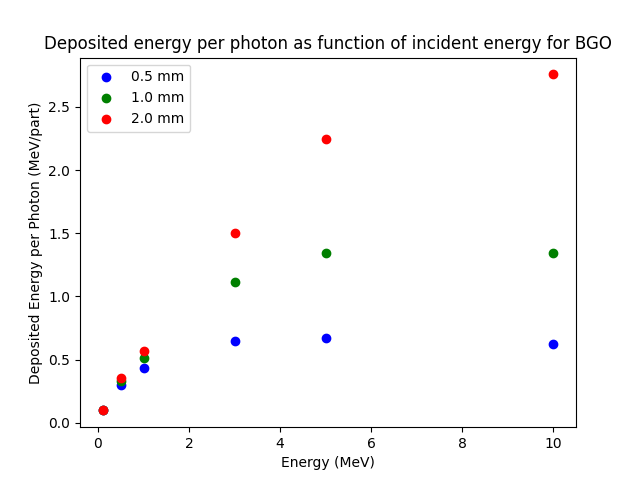
\includegraphics[width=\linewidth]{images/task3/dep_en_BGO.png}
  \caption{}
\end{subfigure}%
\begin{subfigure}{.5\textwidth}
  \centering
  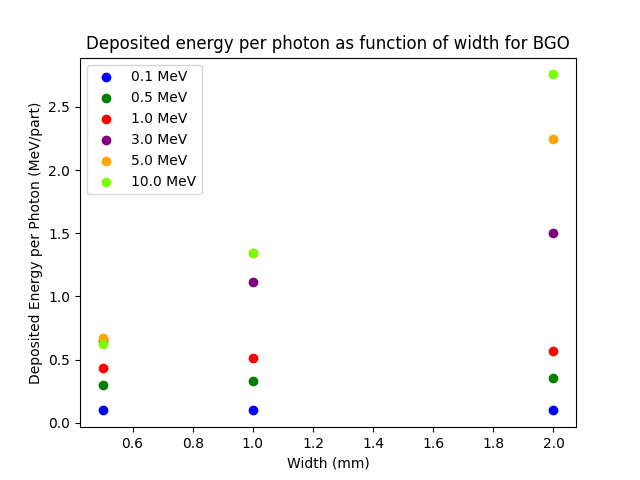
\includegraphics[width=\linewidth]{images/task3/dep_en_width_BGO.png}
  \caption{}
\end{subfigure}
\caption{Deposited energy per photon – BGO}
\end{figure}

\begin{figure}[H]
\centering
\begin{subfigure}{.5\textwidth}
  \centering
  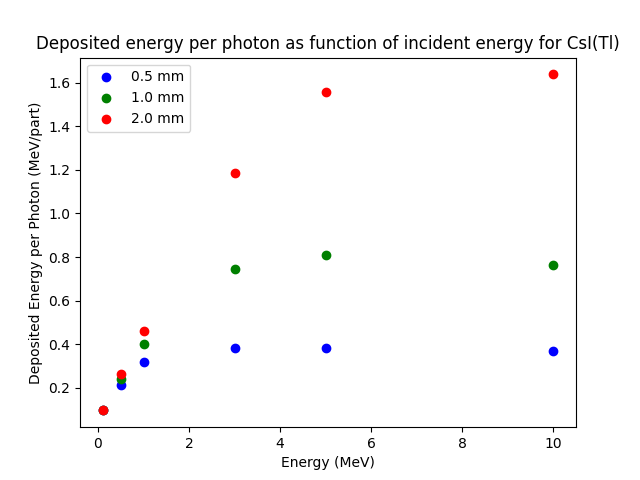
\includegraphics[width=\linewidth]{images/task3/dep_en_CsI.png}
  \caption{}
\end{subfigure}%
\begin{subfigure}{.5\textwidth}
  \centering
  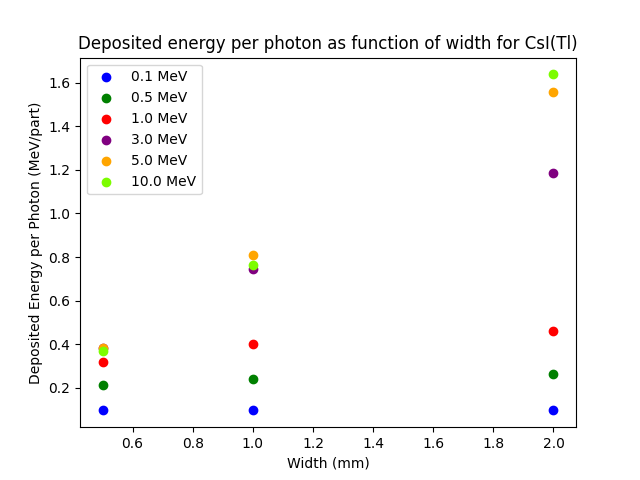
\includegraphics[width=\linewidth]{images/task3/dep_en_width_CsI.png}
  \caption{}
\end{subfigure}
\caption{Deposited energy per photon – CsI(Tl)}
\end{figure}

\begin{figure}[H]
\centering
\begin{subfigure}{.5\textwidth}
  \centering
  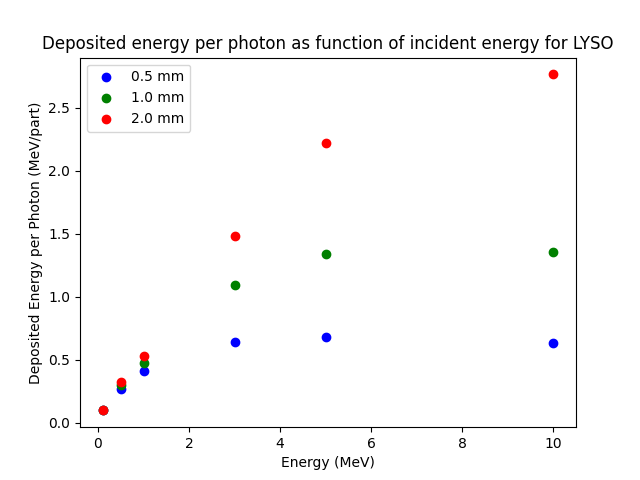
\includegraphics[width=\linewidth]{images/task3/dep_en_LYSO.png}
  \caption{}
\end{subfigure}%
\begin{subfigure}{.5\textwidth}
  \centering
  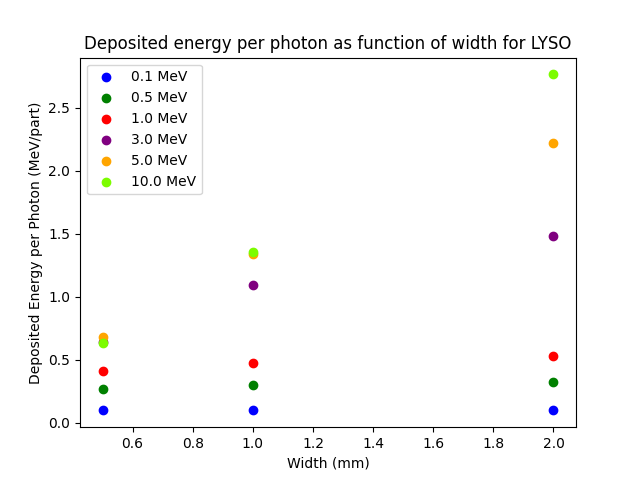
\includegraphics[width=\linewidth]{images/task3/dep_en_width_LYSO.png}
  \caption{}
\end{subfigure}
\caption{Deposited energy per photon – LYSO}
\end{figure}

\begin{figure}[H]
\centering
\begin{subfigure}{.5\textwidth}
  \centering
  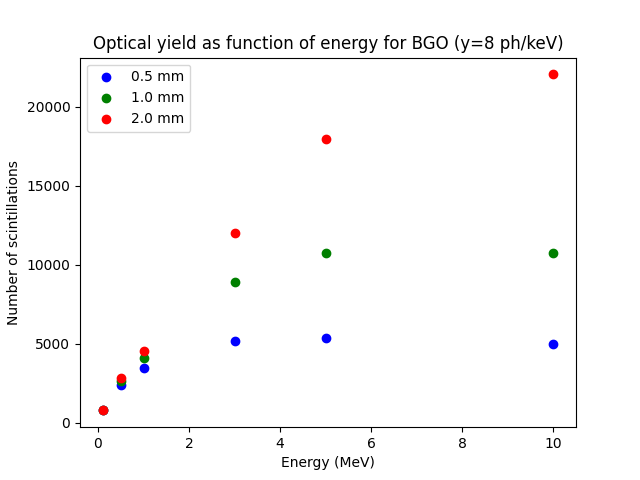
\includegraphics[width=\linewidth]{images/task3/scintills_energy_BGO.png}
  \caption{}
\end{subfigure}%
\begin{subfigure}{.5\textwidth}
  \centering
  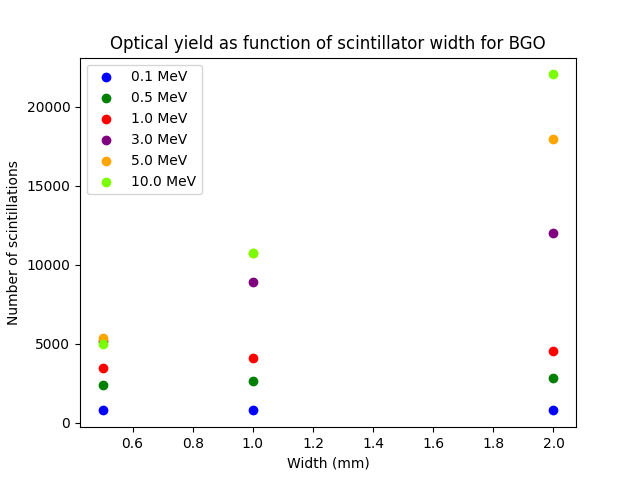
\includegraphics[width=\linewidth]{images/task3/scintills_width_BGO_part.png}
  \caption{}
\end{subfigure}
\caption{Optical yield per photon - BGO}
\end{figure}

\begin{figure}[H]
\centering
\begin{subfigure}{.5\textwidth}
  \centering
  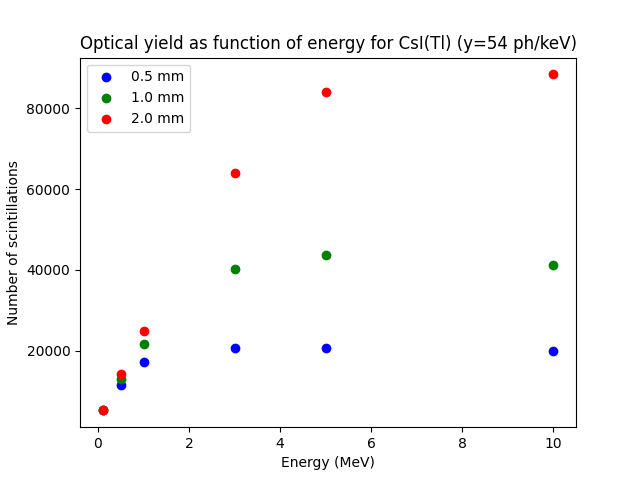
\includegraphics[width=\linewidth]{images/task3/scintills_energy_CsI.png}
  \caption{}
\end{subfigure}%
\begin{subfigure}{.5\textwidth}
  \centering
  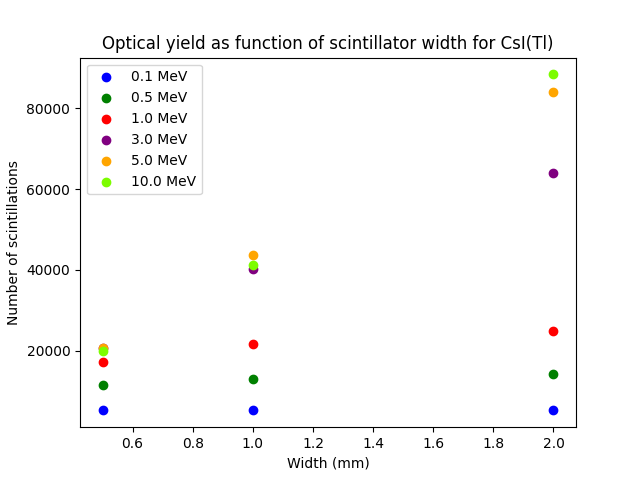
\includegraphics[width=\linewidth]{images/task3/scintills_width_CsI_part.png}
  \caption{}
\end{subfigure}
\caption{Optical yield per photon - CsI(Tl)}
\end{figure}

\begin{figure}[H]
\centering
\begin{subfigure}{.5\textwidth}
  \centering
  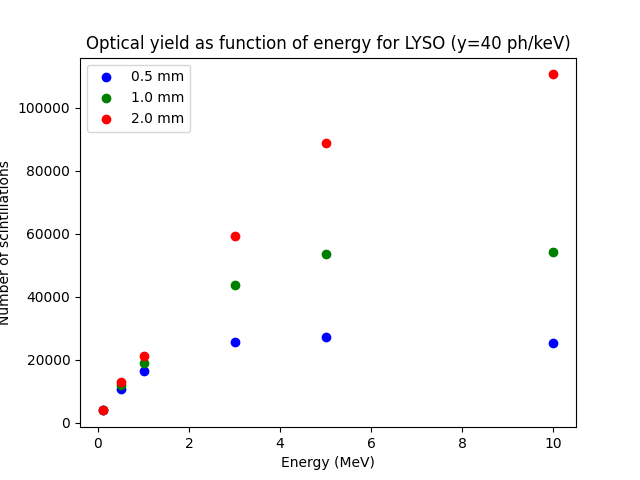
\includegraphics[width=\linewidth]{images/task3/scintills_energy_LYSO.png}
  \caption{}
\end{subfigure}%
\begin{subfigure}{.5\textwidth}
  \centering
  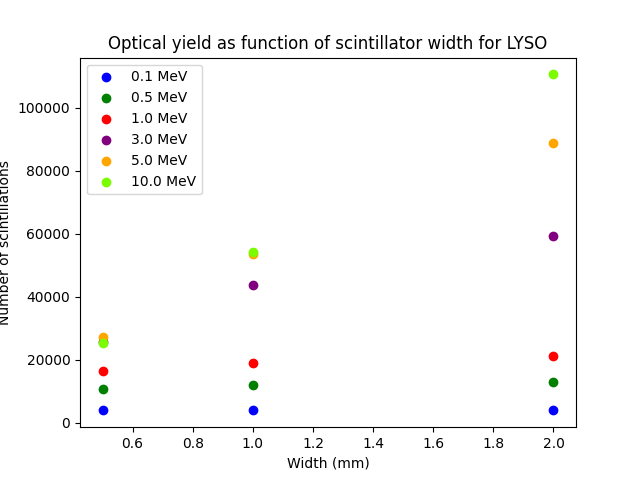
\includegraphics[width=\linewidth]{images/task3/scintills_width_LYSO_part.png}
  \caption{}
\end{subfigure}
\caption{Optical yield per photon - LYSO}
\end{figure}

\begin{figure}[H]
  \centering
  \includegraphics[width=\linewidth]{images/task3/deposited_energy_all.pdf}
  \caption{Deposited energy per photon for each scintillator material and detector thicnkess as function of incident photon energy. In these simulations,
  we used a beam of $10^6$ incident photons. }
   % \label{fig:bgo2mm}
\end{figure}

\begin{figure}[H]
  \centering
  \includegraphics[width=\linewidth]{images/task3/optical_yield_all.pdf}
  \caption{The total optical yield (total number of scintillations produced by the beam, not per incident photon) for each scintillator material and detector thicnkess as function of incident photon energy. In these simulations,
  we used a beam of $10^6$ incident photons. }
   % \label{fig:bgo2mm}
\end{figure}

\subsection{Task 4. Surface energy deposition}

Simulations were performed for the following materials: CsI(Tl), BGO, LYSO. The thicknesses 
of the scintillator were 0.5, 1 and 2 mm. The energies used for the incident photons were 0.1, 0.5, 1, 3, 5 and 10 MeV. 
The simulations were performed for $10^7$ incident photons. The results are presented in the following figures.

\begin{figure}[H]
  \centering
    \includegraphics[width=\linewidth]{images/task4/surface_CsI_10_2.png}
    \caption{2D energy deposition for a beam of $10^7$ photons of 10 MeV in a 2mm thick CsI scintillator.}
    % \label{fig:bgo2mm}
\end{figure}
\begin{figure}[H]
  \centering
    \includegraphics[width=\linewidth]{images/task4/logsurface_CsI_10_2.png}
    \caption{Log scale view of the energy deposition.}
    % \label{fig:bgo2mm}
\end{figure}

What I added new to the code:

\begin{itemize}
  \item I included a \verb|config.json| file where the parameters of interest can be modified (so far, beam energy, detector thickness and material)
  \item in the root file, there can be found 3 histograms: 1D energy deposition histogram, 2D surface energy deposition histogram and another histogram 
  from which we can identify the energy of the beam and number of particles
  \item in \verb|SteppingAction.cc|, modified \\ \verb|G4ThreeVector position = aStep->GetPostStepPoint()->GetPosition();| in order to obtain a better projection shape that can be fitted with a function
\end{itemize}

The first 3 figures show the X projection of the 2D energy deposition histogram for each scintillator material and detector thickness. From these projections,
the FWHM and FWTM was computed analitically and plotted in the last 2 figures. The next step is to compare this values with the ones obtained from fitting.

\begin{figure}[H]
    \centering
    \includegraphics[width=\linewidth]{images/task4/BGO_2mm.pdf}
    \caption{X projection of the 2D energy deposition histogram for BGO scintillator at 2mm detector thickness.}
    % \label{fig:bgo2mm}
\end{figure}
\begin{figure}[H]
    \centering
    \includegraphics[width=\linewidth]{images/task4/LYSO_2mm.pdf}
    \caption{X projection of the 2D energy deposition histogram for LYSO scintillator at 2mm detector thickness.}
    % \label{fig:bgo2mm}
\end{figure}
\begin{figure}[H]
    \centering
    \includegraphics[width=\linewidth]{images/task4/CsI_2mm.pdf}
    \caption{X projection of the 2D energy deposition histogram for CsI(Tl) scintillator at 2mm detector thickness.}
    % \label{fig:bgo2mm}
\end{figure}


\begin{figure}[H]
    \centering
    \includegraphics[width=\linewidth]{images/task4/FWHM_all.pdf}
    \caption{Full width at half maximum for all scintillators and all energies.}
    % \label{fig:bgo05mm}
\end{figure}

\begin{figure}[H]
    \centering
    \includegraphics[width=\linewidth]{images/task4/FWTM_all.pdf}
    \caption{Full width at tenth maximum for all scintillators and all energies.}
    % \label{fig:bgo05mm}
\end{figure}

Notes 25 ianuarie:

\begin{itemize}
  \item de repetat simularile CsI 2 mm si 1 mm
  \item grafic, cum arata proiectia in fct de distanta si ca fwtm e exact ce da script-ul
  \item la 10 MeV verifica valoarea obtinuta
  \item CsI 3 MeV 5 MeV - ceva nu este in regula
  \item de verificat ca script-ul face ce trebuie
\end{itemize}



Ar trebui calculata en depusa. Pentru fiecare FWTM si FWHM calculat, sa se calculeze si energia depusa. Rezolutie vs eficienta
Incearca super gaussian fit.

Energia depusa in zona FWTM. Gaseste markerii care definesc FWTM sau FWHM si calc energia depusa intre ei (integreaza) si compara cu energia depusa totala (pot s ao iau si din 1D).

Scopul este sa vedem cata energie se depune in zona de interes (fwtm) si cata energie ramane in rest (asta e zgomotul).

Semnal zgomot.

To be continued with Super Gaussian fit.


\end{document}
